%  This LaTeX template is based on T.J. Hitchman's work which is itself based on Dana Ernst's template.  
% 
% --------------------------------------------------------------
% Skip this stuff, and head down to where it says "Start here"
% --------------------------------------------------------------
 
\documentclass[12pt]{article}
 
\usepackage[margin=1in]{geometry} 
\usepackage{amsmath,amsthm,amssymb}
\usepackage{braket}
\usepackage{tikz}
\usepackage{quiver}
\usetikzlibrary{calc}
\usepackage{listings}
\usepackage{graphicx}
\usepackage[utf8x]{inputenc}
\usepackage[english]{babel}
\usepackage{bbm}
\usepackage{dsfont}
\usepackage{makecell}
\usepackage{hyperref}
\usepackage{float}
\usepackage{siunitx}
\usepackage{multirow}
\usepackage{ mathrsfs }
\usepackage{circuitikz}
\usepackage{siunitx}

\usetikzlibrary{calc}
\usetikzlibrary{shapes}
\usetikzlibrary{shapes.callouts}

\theoremstyle{remark}
\newtheorem*{theorem}{Theorem}
\newenvironment{statement}[2][Statement]{\begin{trivlist}
\item[\hskip \labelsep {\bfseries #1}\hskip \labelsep {\bfseries #2.}]}{\end{trivlist}}
\newcommand{\diffn}[1]{\,\mathrm{d}{#1}}
\newcommand{\fdiffn}[2]{\frac{\diffn{#1}}{\diffn{#2}}}
\newcommand{\parens}[1]{\left({#1}\right)}
\newcommand{\shrug}[1][]{%
\begin{tikzpicture}[baseline,x=0.8\ht\strutbox,y=0.8\ht\strutbox,line width=0.125ex,#1]
\def\arm{(-2.5,0.95) to (-2,0.95) (-1.9,1) to (-1.5,0) (-1.35,0) to (-0.8,0)};
\draw \arm;
\draw[xscale=-1] \arm;
\def\headpart{(0.6,0) arc[start angle=-40, end angle=40,x radius=0.6,y radius=0.8]};
\draw \headpart;
\draw[xscale=-1] \headpart;
\def\eye{(-0.075,0.15) .. controls (0.02,0) .. (0.075,-0.15)};
\draw[shift={(-0.3,0.8)}] \eye;
\draw[shift={(0,0.85)}] \eye;
% draw mouth
\draw (-0.1,0.2) to [out=15,in=-100] (0.4,0.95); 
\end{tikzpicture}}
\begin{document}
 
% --------------------------------------------------------------
%
%                         Start here
%
% --------------------------------------------------------------
\title{Info Theory Notes 2: Electric Boogaloo}
\author{Rohan Ramkumar, Grant Yang, Atharv Goel}
\maketitle
\tableofcontents
\newpage
\section{Rate Distortion Theory}
\subsection{Generalized Entropy and Capacity (01.13.2025)}

\begin{itemize}
    \item Source $\to$ Source + cost function $b(x)$.
    \item Entropy $H(X)$ $\to$ Generalized entropy $H(X,\delta)\triangleq R(\delta)$ where $\delta$ is the upper bound of the distortion that I'm willing to tolerate.
    \item Channel $\to$ Channel + distance function $d(x,y).$ This function represents how unhappy we are with the distortion. 
    \item Channel capacity $C(Y|X)$ $\to$ generalized channel capacity $C(Y|X,\beta)\triangleq C(\beta),$ where $\beta$ is the bound on the power available at the source.
\end{itemize}
 

\textbf{More rigorous definition:}
Recall the Mutual Information $I(X;Y),$ and that $C(Y|X)=\max_{X}{I(X;Y)}.$ We also can think of $H(X)$ as the minimum of $I(X;Y)$ over all channels that effectively result in $Y=X$ (that do not do anything). With generalized entropy this is useful but with normal stuff, $I(X;Y) = H(X)$ for all such trivial channels.

We have $H(X,\delta)=R(\delta).$ First, we pick an arbitrary $\delta,$ which is the acceptable distortion. Specifically, we cannot tolerate an average distortion of more than $\delta.$ If our distortion function is $d(x,y),$ then our average distortion is
\[\bar{d}=E_{X,Y}[d(x,y)].\]

Now, we have to design the system so that our average distortion is less than $\delta.$ So, we consider the channels such that $\bar{d}\le\delta.$ Of these channels, we choose the one with minimum $I(X;Y),$ and we define this to be $H(X,\delta)=R(\delta)$ (we try to compress our source as much as possible given our tolerance for distortion $\delta$).

Channel Capacity:
$C(\beta)=C(Y|X,\beta).$ Choose an arbitrary $\beta,$ which is the average cost greater than which we cannot tolerate. Letting
\[\bar{b}=E_X[b(x)].\] We only consider the sources for which $\bar{b}\le\beta,$ and we choose the one that maximizes mutual information $I(X;Y).$ This value is $C(\beta)$ and analogous to normal channel capacity.

There is a generalized source coding theorem \url{https://en.wikipedia.org/wiki/Rate%E2%80%93distortion_theory} \shrug[].

Chat, what does $R(\delta)$ look like? It can be proven that it is decreasing and convex.

\begin{figure}[H]
    \centering
    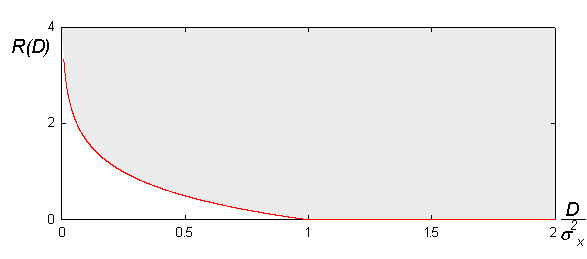
\includegraphics[width=0.5\linewidth]{generalizedEntropy.png}
    \caption{$R(\delta)$ decreases as more distortion being acceptable means we can get away with sending less info. Instead of an x-intercept at $1$ it's at $\delta_{max}$ or something. The y-intercept is $H(X).$}
    \label{fig:genentropy}
\end{figure}



\begin{figure}[H]
\centering
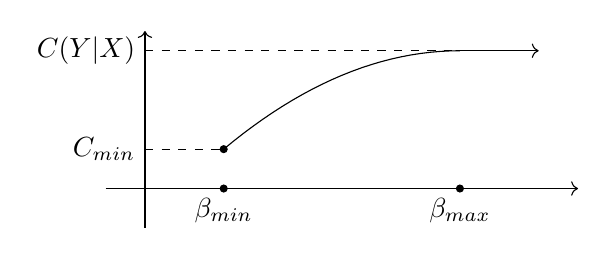
\begin{tikzpicture}
\draw[->] (-0.5, 0) -- (5.5, 0);
\draw[->] (0, -0.5) -- (0, 2);
\filldraw (1, 0) circle (1.25pt) node[anchor=north] {$\beta_{min}$} (4, 0) circle (1.25pt) node[anchor=north] {$\beta_{max}$};
\draw[dashed] (0, 1.75) -- (5, 1.75) (0, 0.5) -- (1, 0.5);
\draw plot[domain=-1:0] ({4+3*\x},{1.75-1.25*\x*\x});
\draw[->] (4, 1.75) -- (5,1.75);
\filldraw (0, 0.5) node[anchor=east] {$C_{min}$} (0, 1.75) node[anchor=east] {$C(Y|X)$} (1,0.5) circle (1.25pt);
\end{tikzpicture}
\caption{What does $C(\beta)$ look like? Similar but not the same. Apparently it is concave and increasing.}
\end{figure}


Binary source:
1 with probability $p$ and 0 with probability $1-p,$ where $p\le\frac{1}{2}.$
Our claim is that
\[R(\delta)=\begin{cases}H(p)-H(\delta)&0\le\delta<p\\0&\delta\ge p\end{cases}.\]
We define our distortion function
\[d(X,Y)=X\oplus Y=\begin{cases}0&X=Y\\1&X\ne Y\end{cases}.\] For each source-channel combination
TODO: COPY OLD IMAGE WITH SOURCE AND CHANNEL.

We have two numbers: $I(X;Y)$ and $E_{XY}[d(X,Y)].$ Ignore any channel that has a worse distortion than $\delta.$ This lets you find $R(\delta_0)$ for all $\delta_0.$ But this is not fun, so we will be smart about it.


Part 1:
Claim: No matter what test channel we connect to the source when measuring $I(X;Y)$ and $E[\cdot],$ you will find that
\[I(X;Y)+H(E_{XY}[d(X,Y)])\ge H(p).\] Since $0\le d\le 1$ we can pretend it's a random variable. 
We have
\begin{align*}I(X;Y)&=H(X)-H(X|Y)\\
&=H(p)-H(X|Y)\\
&=H(p)-H(X\oplus Y|Y)\\
&\ge H(p)-H(X\oplus Y)\\
% &=H(p)-H(\text{a Random Variable that is 1 when X$\ne$ Y and 0 when X=Y})\\
% &=H(p)-H(\text{a Random Variable that is 1 when d(x,y)=1 and 0 when d(x,y)=0})\\
% &=H(p)-H(\text{a different ``p'' that is the probability that d(x,y)=1})\\
&=H(p)-H(E_{XY}[d(X,Y)]),
\end{align*}
\[\therefore I(X;Y)+H(E_{XY}[d(X,Y)])\ge H(p).\label{bsrcpt1}\]

\subsection{More $R(\delta)$ (01.15.2025)}

Binary Source Review:
We want to prove that
\[R(\delta)=\begin{cases}
    H(p)-H(\delta)&0\le\delta<p\\
    0&\delta\ge p
\end{cases}.\]
Part 1:
From Monday we have
\[I(X;Y)+H(E_{XY}[d(X,Y)])\ge H(p).\]

Now we only consider the channels that yield an expected distortion $\bar{d}=E_{XY}[d(X,Y)]\le\delta,$ where $\delta\le\frac{1}{2}$ because $H(p)$ is monotonic until $\frac{1}{2}.$ (If $\delta>\frac{1}{2}$ then what? ...) Because

\[I(X;Y)\ge H(p)-H(\delta),\] the minimum of $I(X;Y),$ which is $R(\delta),$ must also be greater than $H(p)-H(\delta).$ But, we need to prove that this minimum value is actually achieved.

Part 2:
Claim: As long as $\delta\le p,$ then there must exist a channel (which we can construct) with the following properties:
\begin{enumerate}
    \item This channel has an expected distortion of exactly $\delta$
    \item This channel has has a mutual information of exactly $H(p)-H(\delta).$
\end{enumerate}

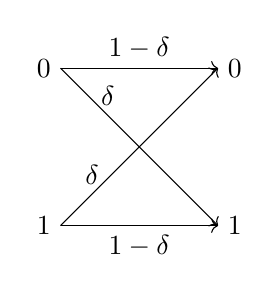
\begin{tikzpicture}[scale=2.0]
    \draw (0,0) node[anchor=east] {1} (0,1) node[anchor=east] {0} (1,0) node[anchor=west] {1} (1,1) node[anchor=west] {0};
    \draw[->] (0, 0) -- node[pos=0.2,above] {$\delta$} (1,1);
    \draw[->] (0, 0) -- node[below] {$1-\delta$} (1,0);
    \draw[->] (0, 1) -- node[pos=0.3,above] {$\delta$} (1,0);
    \draw[->] (0, 1) -- node[above] {$1-\delta$} (1,1);
\end{tikzpicture}
Considering a source with probability $p$ of outputting 0, along with a mystery channel. We compose this channel with a BSC with probability $\delta.$
\[\text{Source}\to X\to \text{Mystery Channel}\to Y\to\text{BSC}_\delta\to Z\]
(This part is weird) We want $Z=X,$ so that
\[P(Z=0)=p,P(Z=1)=1-p.\]
If this is possible, then (apparently) we will have solved our problem, i.e. $R(\delta)=H(p)-H(\delta).$ The expected distortion will be exactly $\delta.$ But, the proof doesn't matter.


Example 2:
Consider the source such that
\[P(X=x)=\frac{1}{3}\] for $x\in \{-1,0,1\},$ and let the output be $y\in\{-\frac{1}{2},\frac{1}{2}\}.$

We have the distortion matrix
\[\begin{bmatrix}
    1&2\\
    1&1\\
    2&1
\end{bmatrix}.\]
Guess that \[P(Y|X)=\begin{bmatrix}
    \alpha&1-\alpha\\
    0.5 &0.5\\\
    1-\alpha&\alpha
\end{bmatrix},\]
based off the distortion function. We have
\[I(X;Y)=H(Y)-H(Y|X)=1-\left(\frac{2}{3}H(\alpha)+\frac{1}{3}H(0.5)\right)=\frac{2}{3}-\frac{2}{3}H(\alpha).\]

Next, we want $\bar{d}.$ We just overlay the distortion matrix on top of the $P(Y|X)$ matrix, multiplying elements and adding them together and dividing by 3. This is because $\bar{d} = \sum p(x,y) d(x,y)$ and $p(x,y) = p(x) p(y|x) = \frac{1}{3} p(y|x)$. This is just \[1+\frac{2}{3}(1-\alpha)=\frac{5}{3}-\frac{2}{3}\alpha.\] Now, we minimize $I(X;Y)$ such that $\bar{d}\le\delta.$
This means that
\[\alpha\ge\frac{5-3\delta}{2}.\] Since $0\le \alpha\le \frac{1}{2},$ we must have
\[1\le\delta\le\frac{4}{3}.\]

\paragraph{Gaussian Source}
Consider a source that is distributed as a guassian with mean $0$ and variance $\sigma^2.$ We claim that
\[R(\delta)=H(X,\delta)=\begin{cases}
    \frac{1}{2}\log\frac{\sigma^2}{\delta}&0\le\delta\le\sigma^2\\
    0&\delta>\sigma^2
\end{cases},\]

where the distortion function is mean-squared error:
\[d(x,y) = (x-y)^2.\]

We have
\begin{align*}I(X;Y)&=h(X)-h(X|Y)=\frac{1}{2}\log(2\pi e\sigma^2)-h(X|Y)\\&=\frac{1}{2}\log(2\pi e\sigma^2)-h((X-Y)|Y)\\&\ge \frac{1}{2}\log(2\pi e\sigma^2)-h(X-Y)\\
&\ge \frac{1}{2}\log(2\pi e\sigma^2)-h\left(N\left(0, \mathrm{E}\left[(X-Y)^2\right]\right)\right)\\
&=\frac{1}{2}\log(2\pi e\sigma^2)-\frac{1}{2}\log\left(2\pi e\,\mathrm{E}\left[(X-Y)^2\right]\right),
\end{align*}
since normal distribution has max entropy we can replace $X-Y$ with a gaussian of the same variance, and here we assume that $E[X] = E[Y] = 0$.
Thus,
\[R(\delta)\ge\frac{1}{2}\log\frac{\sigma^2}{\delta}.\]
\subsection{More Gaussian Sources and Capacity Cost (1.17.2025)}
\paragraph{Capacity Cost Functions}
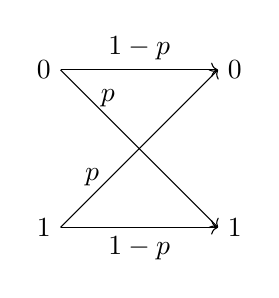
\begin{tikzpicture}[scale=2.0]
    \draw (0,0) node[anchor=east] {1} (0,1) node[anchor=east] {0} (1,0) node[anchor=west] {1} (1,1) node[anchor=west] {0};
    \draw[->] (0, 0) -- node[pos=0.2,above] {$p$} (1,1);
    \draw[->] (0, 0) -- node[below] {$1-p$} (1,0);
    \draw[->] (0, 1) -- node[pos=0.3,above] {$p$} (1,0);
    \draw[->] (0, 1) -- node[above] {$1-p$} (1,1);
\end{tikzpicture}
Our cost function is
\[\begin{cases}0&x=0\\1&x=1\end{cases}\].
We limit the sources to those with average cost $\beta,$ and we want to maximize $I(X;Y).$
We claim that
\[C(\beta)=\begin{cases}H[(1-\beta)(1-p)+\beta p]-H(p)&0\le\beta\le\frac{1}{2}\\1-H(p)&\beta\ge\frac{1}{2}\end{cases}.\]
Assume $X$ is a binary source with
\[X=\begin{cases}0&1-p_s\\1&p_s\end{cases}.\]
We have
\[I(X;Y)=H(Y)-H(Y|X)=H((1-p_s)(1-p)+p_sp)-H(p).\] Since the average cost $\bar{b}=p_s,$ so if $\bar{b}<\beta,$ then we just need $p_s<\beta.$ Since $H(p)$ is maximized at $p=\frac{1}{2},$ we want to get $(1-p_s)(1-p)+p_sp=\frac{1}{2}.$

If $\beta>\frac{1}{2},$ we can just set $p_s=\frac{1}{2},$ and this is the maximum. If $\beta<\frac{1}{2},$ we can set $p_s=\beta.$
\paragraph{Example}
Let $X:\{0,\frac{1}{2},1\}$ and $Y:\{0,1\}.$ Our transition matrix is
\[\begin{bmatrix}
    1&0\\
    \frac{1}{2}&\frac{1}{2}\\
    0&1
\end{bmatrix}.\]
Our cost function is $b(0)=b(1)=1,b(\frac{1}{2})=0.$
First we find the mutual information, guessing that the distribution of $X$ is \[\left(\alpha, 1-2\alpha, \alpha\right).\]
\[I(X;Y)=H(Y)-H(Y|X)=1-1(1-2\alpha)=2\alpha.\]
Our average cost is
\[\bar{b}=2\alpha=I(X;Y),\]
so $C(\beta)=\beta.$


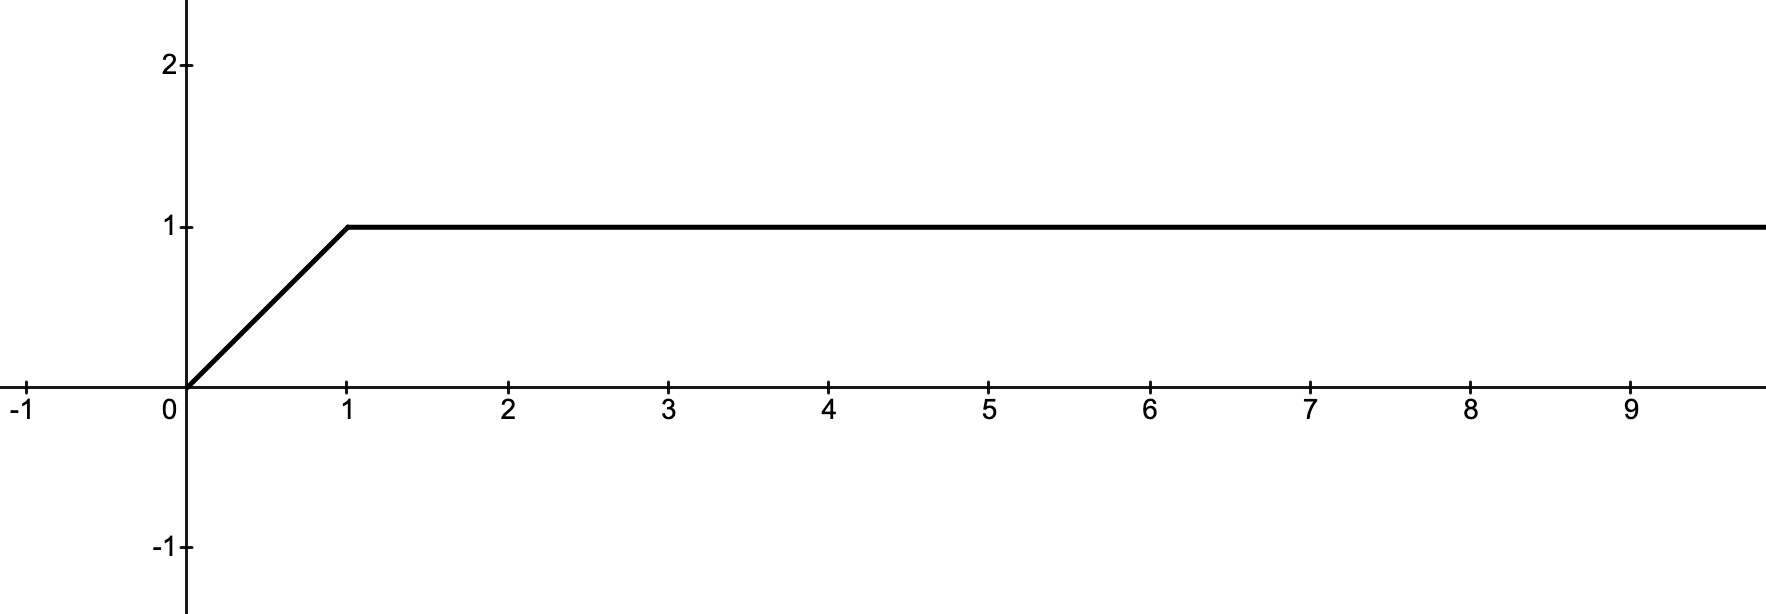
\includegraphics[width=\textwidth]{TernaryCapacityCostExample.png}.
\paragraph{Gaussian Channel}
Consider a gaussian channel that adds $Z\sim N(0,\sigma^2)$ to $X$ to output $Y,$ with a cost function of $b(x)=x^2.$ We have
\begin{align*}I(X;Y)&=h(y)-h(Y|X)\\&=h(Y)-h(X+Z|X)\\&=h(Y)-H(Z|X)\\&=h(Y)-h(Z)\\&=h(Y)-\frac{1}{2}\log(2\pi e\sigma^2).\end{align*}
Assuming that a source has a variance $\sigma_s^2.$ Since the source and noise are independent,
\[\mathrm{Var}[Y]=\mathrm{Var}[X]+\mathrm{Var}[Z]=\sigma_s^2+\sigma^2.\]

So, the maximum entropy of $Y$ must be
\[\frac{1}{2}\log(2\pi e(\sigma_s^2+\sigma^2)),\]
and so
\[I(X;Y)\le \frac{1}{2}\log(2\pi e(\sigma_s^2+\sigma^2))-\frac{1}{2}\log(2\pi e\sigma^2).\] If $\mu_X=0,$ we have $E[X^2]=\sigma_s^2$ and $\mathrm{Var}[X] =\sigma_s^2,$ so
\[C(\beta)=\frac{1}{2}\log\left(1+\frac{\beta}{\sigma_s^2}\right).\]
\subsubsection{Homework questions}
\begin{enumerate}
\item \[D=\begin{bmatrix}0&1\\2&0\end{bmatrix},\] with a binary source $X$ such that $p_x=\frac{1}{2}.$ What is $R(\delta)?$
\item Let \[p(y|x)=\begin{bmatrix}q&p&0\\0&p&q\end{bmatrix},\] with $b(0)=0$ and $b(1)=1.$ What is $C(\beta)?$
\end{enumerate}
\subsection{Generalized Shannon Theorem (1.22.2025)}
\paragraph{Homework 2}
Let \[p(y|x)=\begin{bmatrix}q&p&0\\0&p&q\end{bmatrix},\] with $b(0)=0$ and $b(1)=1.$ What is $C(\beta)?$

Let $P(X=0)=\alpha$ and $P(X=1)=1-\alpha.$
\begin{align*}I(X;Y)&=H(Y)-H(Y|X)\\&=H(\alpha q,p,(1-\alpha)q)-H(q)\\&=\alpha q\log\frac{1}{\alpha q}+(1-\alpha)q\log\frac{1}{1-\alpha q}+p\log\frac{1}{p}-H(q)\\&=qH(\alpha).\end{align*}
Or you could save yourself 20 minutes and solve it using $I(X;Y)=H(X)-H(X|Y),$ exercise left for the reader.

We also have
\[\bar{b}=1-\alpha,\] so if $\bar{b}\le\beta,$ we just want to maximize
\[qH(\alpha)\] subject to $(1-\alpha)\le \beta.$ If $\beta\ge\frac{1}{2},$ then let $\alpha=\frac{1}{2},$ with $C(\beta)=qH(\frac{1}{2})=q.$

If $\beta<\frac{1}{2},$ let $\alpha=\beta,$ so $C(\beta)=qH(\beta).$

\paragraph{Homework 1}
(This solution isn't correct but correct enough)
\[D=\begin{bmatrix}0&1\\2&0\end{bmatrix},\] with a binary source $X$ such that $p_x=\frac{1}{2}.$ What is $R(\delta)?$

Let 
\[p(y|x)=\begin{bmatrix}
    q_1&1-q_1\\
    q_2&1-q_2
\end{bmatrix}.\]
We have
\[I(X;Y)=H(Y)-H(Y|X)=H\left(\frac{q_1+q_2}{2}\right)-\left(\frac{1}{2}H(q_1)+\frac{1}{2}H(q_2)\right).\]
We also have
\[\bar{d}=\frac{1}{2}(1-q_1)+q_2.\]
By Jensen, $H(\frac{q_1+q_2}{2})\ge\frac{1}{2}H(q_1)+\frac{1}{2}H(q_2).$ We want to minimize the gap between these two guys, which only occurs when $q_1=q_2,$ in which case
\[\bar{d}=\frac{1}{2}(1+q_2).\] If $\delta\ge\frac{1}{2},$ then we can find a scenario with $q_1=q_2,$ in which case we have a Generalized Entropy of zero.

But if $\delta<\frac{1}{2},$ what do we do? If we set $q_1=0,$ we have $\bar{d}=\frac{1}{2}+q_2,$ but this is always more than $\delta$ :(

If we set $q_2=0,$ we have \[\bar{d}=\frac{1}{2}(1-q_1),\] so if $\bar{d}<\delta,$ we have
\[q_1\ge 1-2\delta.\] (Basically we are shoving $q_2$ to the left in order to minimize the Jensen gap, although this logic is faulty.)

We get
\[I(X;Y)=H\left(\frac{1-2\delta}{2}\right)-\frac{1}{2}H(1-2\delta).\]

It turns out that depending on $\delta,$ we have to make $q_2$ a little more than zero to get the truly optimal solution.

\paragraph{General form of Shannon's Theorem}
Given a source $p(x)$ along with symbol costs $b(x)$, and given a channel $p(y|x)$ along with distortion function $d(x,y)$, we must design an encoder/decoder pair such that the probability of an error is zero.

Our average cost is $\bar{b}=E_X[b(X)]$ and our average distortion is $\bar{d}=E_{XY}[d(X,Y)].$ Remember that a lower $\bar{d}$ means better quality, so we have a trade-off between cost and quality.

\textbf{Generalized Shannon's Theorem:} If and only if $R(\delta)\le C(\beta),$ then there exists an encoder/decoder pair that achieves the cost $\beta$ and distortion $\delta.$ $R$ is decreasing and concave up, while $C$ is increasing and concave down.

\textbf{Graphical Intuition}
We can graph the possible pairs of $\delta$ and $\beta$ depending on whether or not $H_{max}<C_{max}$.

If $H_{max} < C_{max}$, then at $\beta = 0$ we intercept at $\delta_{knee}$ (assuming $C(\beta)$ is not 0 or something I guess). At $\delta = 0$ we are at whatever $\beta$ yields $H_{max}$, which will be slightly less than $\beta_{knee}$.

If $H_{max} > C_{max}$, then we still intercept at $\delta_{knee}$. However, we cannot reach $\delta = 0$. Instead, we reach $\beta_{knee}$ when $\delta$ is somewhere and we stay above it.


\paragraph{Example}
\begin{enumerate}
    \item \[p(y|x)=\begin{bmatrix}
        1&0&0\\
        0&1&0\\
        0&0&1
    \end{bmatrix}.\] We have $b(0)=b(1)=1,$ and $b(2)=4.$ We have $P(X=i)=\alpha_i$ for $i=0,1,2.$ Find $C(\beta).$
    \item \[D=\begin{bmatrix}
        0&1&\frac{1}{4}\\
        1&0&\frac{1}{4}
    \end{bmatrix}.\]
    $p_x=\{\frac{1}{2},\frac{1}{2}\}.$ Find $R(\delta).$
\end{enumerate}

\paragraph{Solution}
\begin{enumerate}
    \item We have 
    \[I(X;Y)=H(X)-H(X|Y)=H(X),\] because $Y=X.$ We want to find maximum value of $H(X)$ with $\bar{b}<\beta.$ By symmetry, $\alpha_0=\alpha_1:=\alpha,$ so $\alpha_2=1-2\alpha,$ so $\bar{b}=2\alpha+4-8\alpha=4-6\alpha<\beta,$ and \[\alpha\ge\frac{4-\beta}{6}.\]

    If $\frac{4-\beta}{6}<\frac{1}{3},$ we can set $\alpha=\frac{1}{3},$ to maximize $H(X)=\log 3.$ This is when $\beta>2.$

    If $\frac{4-\beta}{6}>\frac{1}{3},$ since $H(X)$ is monotonic on $\frac{1}{3}\le \alpha\le\frac{1}{2},$ we can let $\alpha=\min(\frac{4-\beta}{6},\frac{1}{2}),$ and this occurs when $0<\beta<2.$
    
\end{enumerate}

\section{Gambling}
\subsection{Gambling (01.24.25)}
Connections between Gambling and Information theory:
\begin{enumerate}
    \item Duality in growth rate of investment and entropy rate
    \item The value of side information
\end{enumerate}

\paragraph{Horse Racing}
These ideas can be extended to the stock market (you can make a lot of money so pay attention). Let there be $n$ horses in a race, such that the $i$th horse wins with a probability of $p_i,$ and you win $o_i$ in exchange for a $\$1$ bet given that horse $i$ wins.

\smallskip

Terminology: we say ``$a$ for $1$" if you bet $\$1$ ahead of time and win $\$a$ if you win, while we say ``$b$ to $1$" if you don't technically bet anything ahead of time, but you win $\$b$ at the end if you win but have to pay out $\$1$ if you lose.

\smallskip

We make the assumption that we distribute our betting money across all the horses, and we let $b_i$ to be the fraction of our money invested on the $i$th horse, where $b_i\ge0$ and $\sum_i b_i=1.$ After the race, you get $b_io_i$ of your buy-in if the $i$th horse wins.

Let the winnings at the end of the race be a random variable, and we wish to maximize the expected value of this variable.

We will repeatedly gamble with a possibly different strategy each time. If we repeatedly gamble, the wealth is the product of our gains, where each gain contributes a factor of $b_i o_i.$ Let $X_1,X_2,X_3,\dots$ be the outcomes of each race, so they are iid. Define the ``wealth relative'' function to be
\[S(X)=b(X)o(X),\] which is the factor by which our wealth grows. We define $S_n$ to be the gambler's wealth after $n$ races, so
\[S_n=\prod_{i=1}^nS(X_i).\]

We define the doubling rate of a race to be
\[W(b,p) = E[\log_2 S(X)]=\sum_{k=1}^mp_k\log_2 (b_ko_k).\]
What does this mean? Why is this a doubling rate? We will work backwards.
\begin{theorem}
Let the race outcomes $X_1,X_2,\dots,X_n$ be i.i.d. according to some distribution $p(x).$ Assume the gambler is using a betting strategy $b,$ where $b$ is a vector of distributions. Then the wealth grows exponentially according to
\[E[S_n]\sim 2^{nW(b,p)}.\]
\end{theorem}
Since the $X_i$ are i.i.d., so are the $\log S(X_i).$ We calculate the doubling rate after playing the game $n$ times:
\[W(n) = \frac{\log_2 S_n}{n}=\frac{1}{n}\sum\log S(X_i).\]

By the weak law of large numbers, this will approach $E[\log S(X)].$ This proves the doubling law. By the monotonicity of $2^x,$ we only have to maximize $W$ to maximize $S_n.$

We want to find $W^\ast(p)$, which is the greatest doubling rate over all choices of $b.$ Specifically,
\[W^\ast(p)=\max_b W(b,p)=\max_{\substack{b:b_i\ge 0\\\sum b_i=1}}\sum p_i
\log b_io_i.\]
We have 
\[\mathcal{L}(b)=\sum p_i\log p_io_i + \lambda\left(\sum_i b_i-1\right),\]
\[\frac{\partial\mathcal{L}}{\partial b_i}=\frac{p_i}{b_i}+\lambda = 0\]
\[\therefore b_i=-\frac{p_i}{\lambda},\] and since $\sum b_i=1,$ we have $\lambda=-1$ and $b_i^\ast=p_i.$ Notice how $b_i$ does not depend on $o_i!!!!$

Thus, since
\[W= \sum p_i\log b_io_i,\]
we know that the optimal doubling rate is:
\[W^\ast=\sum p_i\log o_i-H(p).\] where $b^\ast=p.$
How? Well,
\begin{align*}W(b,p)&=\sum p_i\log b_io_i\\&=\sum p_i\log\left(\frac{b_i}{p_i}\cdot p_io_i\right)\\&=\sum p_i\log o_i-H(p) - D(p||b)\\&\le\sum p_i\log o_i-H(p),\end{align*}
since KL divergence is nonnegative, with equality only when $b_i=p_i.$





What does it mean for something to have fair odds:
\[\sum\frac{1}{o_i}=1.\] We let
\[r_i=\frac{1}{o_i},\] so $r_i$ what the bookie estimates the win probability to be.
We have
\begin{align*}W(b,p)&=\sum p_i\log b_i o_i\\&=\sum p_i\log\frac{b_i}{r_i}\\&=\sum p_i\log\frac{p_i}{r_i}-\sum p_i\log\frac{p_i}{b_i}\\
&=D(p||r)-D(p||b),\end{align*} so the doubling rate is how much worse the bookie's guess of the distribution is than yours.

If the odds are uniformly $m$ for 1, then
\[W^\ast(\vec p)=\log m-H(\vec p),\]
\[W^\ast(\vec p)+H(\vec p)=\log m.\] So, to make the doubling rate go up, we need the entropy to go down.

\subsection{Side Information (1.28.2025)}
\subsubsection{Yesterday's Homework}
Recall that if the bookie assumes odds of $r,$ our doubling rate is
\[W(b,p)=D(p||r)-D(p||b).\]
\[\sum \frac{1}{o_i}=1. \qquad{\text{(Fair odds)}}\]
\[S(X) = b(0)+b(X)o(X).\]

If odds are fair, then it doesn't matter what $b(0)$ is, you can just imagine as if you have less money. So, bet proportional to $p_i$ with the amount of money left ($1-b(0)$).

If odds are in your favor, $\sum \frac{1}{o_i}<1$. Since it's in your favor, you should bet everything ($b(0)=0.$) It doesn't make any sense to save money. Now we do it more rigorously:
\begin{align*}W(b,p)&=\sum p_i\log(b_0+b_io_i)\\&=\sum p_i\log\frac{b_0/o_i+b_i}{1/o_i}\\&=\sum p_i\log\left(\frac{{b_0}/{o_i}+b_i}{p_i}\cdot\frac{p_i}{{1}/{o_i}}\right)\\&=\sum p_i\log p_io_i+\log K-D(p||r),\end{align*}
\[r_i = \frac{b_0/o_i+b_i}{K}\]
\[K=\sum \left(b_0/o_i + b_i\right)=b_0\sum \frac{1}{o_i}+\sum b_i=b_0\left(\sum\frac{1}{o_i}-1\right)+1\]

If we want to maximize $W$ w.r.t. $b_i,$ we just want to maximize $K$ and minimize $D(p||r),$ which occurs when $b_0=0.$ 

What if we have bad odds, where
$\sum\frac{1}{o_i}>1$? We would guess that $b(0)=1,$ to maximize $K=b_0\left(\sum\frac{1}{o_i}-1\right)+1,$ but we don't know about $D(p||r),$ so we don't know for sure. 

What we can show is that proportional betting cannot work. We have
$\sum b_i=1$, and we can arrange the horses in decreasing $b_io_i,$ such that the last horse has the worst $b_io_i.$

Consider a new portfolio where
\[b_i'=b_i-\frac{b_m o_m}{o_i},\] where $m$ is the last horse. Since $b_io_i\ge b_m o_m,$ all the $b_i'$ are $\ge 0.$ We then keep the remaining money:
\[1-\sum b_i'=1-\sum_{i=1}^m\left(b_i-\frac{b_m o_m}{o_i}\right)=\sum \frac{b_mo_m}{o_i}.\]

Consider the return on this portfolio:
\[b_i'o_i=\left(b_i-\frac{b_mo_m}{o_i}\right)o_i+\sum \frac{b_mo_m}{o_i}=b_i o_i+b_mo_m\left(\sum\frac{1}{o_i}-1\right).\]
But, since 
$\sum\frac{1}{o_i}>1,$ we must have that 
\[b_i'o_i>b_io_i.\]
So, our new portfolio is better. This means that we can invest some of it, while saving the rest, and actually make a profit at the end. 


\subsubsection{Side Information}
The gambler has some information relevant to the outcome of the race. What is the value of this ``side information?'' We can measure this by measuring the increase in the doubling rate given the side information.

Let the winning horse be
$X\in\{1,2,\dots,m\}$ with probability $p(X)$ and a return of $o(X)$ for \$1. Our side information is $y$ (for example, this could be previous race history). Define $b(x|y)$ to be the proportion of wealth bet on horse $x$ given some side information $y.$ 
We have $\sum b(x|y)=1$, with $b(x|y)\ge 0.$
We also have
\[W^\ast(X) = \max_{b(x)}\sum_x p(x)\log b(x) o(x).\]
\[W^\ast(X|Y) = \max_{b(x|y)}\sum_{x,y}p(x,y)\log b(x|y)o(x).\]
\[\Delta W = W^\ast(X|Y)-W^\ast(X).\]

\textbf{Theorem}: The increase in the doubling rate due to side information $Y$ for a horse $X$ is
\[\Delta W=I(X;Y).\]

Just as before, $W^\ast(X|Y)$ is maximized at
\[b^\ast(x|y)=p(x|y).\]
\begin{align*}W^\ast(X|Y)&=\max_{b(x|y)}\sum_{x,y} p(x,y)\log \left(b(x|y) o(x)\right)\\&=\sum_{x,y} p(x,y)\log\left(o(x)p(x|y)\right)\\&=\sum_xp(x)\log o(x)-H(X|Y).\end{align*}

Without side information:
\[W^\ast(X)=\sum p(x)\log o(x)-H(X).\] 
\[\therefore \Delta W= W^\ast(X|Y)-W^\ast(X)=H(X)-H(X|Y)=\boxed{I(X;Y)}.\]

\subsection{Finishing Gambling (1.30.2025)}

\paragraph{Dependent Horse Racing and Entropy}
Assume there is a dependence among races, and let the strategy for betting on each race depend on the results of the previous races, specifically:
\[W^\ast(X_k|X_{k-1},X_{k-2},\dots,X_1).\]
Recall that 
\[W(b,p) = D(p||r) - D(p||b).\] If the $o_i$ are uniform and fair such that $r=(m,m,\dots)$ and $b=p$, we have $D(p||r) = \log m - H(\vec{p})$ and $D(p||b) = 0$:
\[W^\ast(\vec p) + H(\vec p) = \log m,\]
\[\therefore W^\ast(X_k|X_{k-1},X_{k-2},\dots,X_1)=\log m - H(X_k|X_{k-1},\dots,X_1).\]
Consider a different perspective where $S_n = \Pi S(X_i),$ so that
\[\frac{1}{n}E[\log S_n] = \frac{1}{n}\sum E[\log S(X_i)]=\frac{1}{n}\sum(\log m - H(X_k|X_{k-1},\dots X_1)).\]

\[\frac{1}{n}E[\log S_n] + \frac{1}{n} H(X_1,X_2,\dots,X_n) = \log m.\]We call $\frac{1}{n}E[\log S_n]$ the doubling rate and $\frac{1}{n}H(X_1,X_2,\dots,X_n)$ the entropy rate. In effect, this is a conservation law just like we saw before: making more money means entropy must be lower (we know more about the R.V.).


\section{Thermodynamics}
\subsection{Dynamical Systems (02.07.2025)}
First-order Nonlinear System: Lotka-Volterra system: predator-prey system
For example, this can represent the change in population between foxes and rabbits, so as there are more foxes, rabbits will be eaten, but then there are less rabbits so foxes will run out of food and start to die of starvation. But, now that there are less foxes, more rabbits will survive, which gives more food to to foxes and increases fox population, etc.

Prey is $x$ and Predators is $y:$
\[\fdiffn{x}{t}=\alpha x-\beta xy=x(\alpha-\beta y)\qquad \fdiffn{y}{t}=\delta x y - \gamma y=y(\delta x - \gamma).\]
The $\beta xy $ term means that the number of prey decreases as both the number of predator and prey increase.


\begin{figure}
\centering
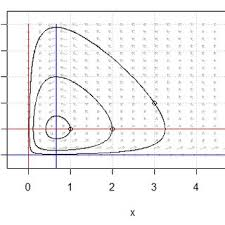
\includegraphics[width = 0.5\textwidth]{lv_system.jpeg}
\end{figure}

Note that they will loop forever (assuming that this system is efficient), and there is an equilibrium point.

The solutions are level curves, so on the level curve,
\[V(x,y) = c.\]
Guess the gradient of $V:$
\[\begin{bmatrix}
    \frac{\partial V}{\partial x}\\
    \frac{\partial V}{\partial y}
\end{bmatrix}=\begin{bmatrix}
    \delta-\frac{\gamma}{x}\\
    \beta - \frac{\alpha}{\gamma}
\end{bmatrix}.\]
Also, we have that
\[\begin{bmatrix}
    \fdiffn{x}{t}\\
    \fdiffn{y}{t}
\end{bmatrix}=\begin{bmatrix}
    \alpha x-\beta xy\\
    \delta xy - \gamma y.
\end{bmatrix}.\]
These two vectors are orthogonal because the phase plot arrows are perpendicular to the gradient (i.e. the phase plot arrows are parallel to the level curve). Alternatively, use multivariable chain rule on $V(x,y)=c.$

How do we guess the gradient?
Note that
\[\fdiffn{y}{x}=-\frac{\delta x-\gamma}{\beta y-\alpha}\frac{y}{x}.\]
So,
\[\frac{\beta y-\alpha}{y}\diffn{y} + \frac{\delta x - \gamma}{x}\diffn{x} = 0.\]

Integrating this, we have
\[V(x,y) = \delta x - \gamma \ln  x + \beta y -\alpha \ln y = c.\]

Remember that in the neighborhood of a point, every (differentiable) curve is linear; this is calculus. We will look near the stable points because that tells us the behavior near sinks and sources.

So, we will linearize our non-linear system. Just like finding the tangent line at a point on a curve, we can find the tangent plane of a function of two variables. So, even if a function is nonlinear, we can make it look linear in a small neighborhood of $(x_0,y_0),$ which are the stable points, where $\fdiffn{x}{t}=\fdiffn{y}{t}=0.$

Back to Lotka-Volterra, we have
\[\begin{bmatrix}
    \fdiffn{x}{t}\\\fdiffn{y}{t}
\end{bmatrix}=\begin{bmatrix}
    (\alpha-\beta y)x\\-(\gamma-\delta x)y
\end{bmatrix}.\]
We want to turn this into a linear function, so we find the infinitesimal difference with $\diffn{x}$ and $\diffn{y}:$
\[
\begin{bmatrix}
    (\alpha - \beta(y_0 + \diffn{y}))(x_0+\diffn{x})-(\alpha - \beta y_0)(x_0) \\
    -(\gamma - \delta(x_0 + \diffn{x}))(y_0+\diffn{y})+(\gamma-\delta x_0)y_0
\end{bmatrix}=\begin{bmatrix}
    ?&?\\?&?
\end{bmatrix}\begin{bmatrix}
    \diffn{x}\\\diffn{y}
\end{bmatrix},\]
and doing the math (multivariable Taylor expansion I think), we get
\[\begin{bmatrix}
    \frac{\partial}{\partial x}(\alpha - \beta y)x\vert_{x_0,y_0}&\frac{\partial}{\partial y}(\alpha-\beta y)x\vert_{x_0,y_0}\\
    \frac{\partial}{\partial x}(-(\gamma - \delta x)y)\vert_{x_0,y_0}&\frac{\partial}{\partial y}( - (\gamma-\delta x)y)|_{x_0,y_0}
\end{bmatrix}.\]
This is the Jacobian matrix.

\paragraph{Example}
Let
\[\dot{x} = x(3-x-2y)\]
and
\[\dot{y} = y(2-x-y).\]
First, we want to find the stable points, where $\dot{x}=0,\dot{y}=0.$
We see that the stable points points are $(0,0),(3,0),(0,2),(1,1).$
Consider $(0,0):$
\[J=\begin{bmatrix}
    (3-2x-2y)|_{0,0}&(-2x)\vert_{0,0}\\
    (-y)\vert_{0,0}&(2-x-2y)\vert_{0,0}
\end{bmatrix}=\begin{bmatrix}
    3&0\\
    0&2
\end{bmatrix}.\]
Since the matrix is diagonal, the eigenvalues are $\lambda=3, 2.$ You can figure out what eigenvalues are if you don't know, just watch the 3b1b video. I believe in you.

Since the eigenvalues are positive, if you place a marble near the stable point, the marble will move away regardless of which direction you place it in.

Now, $(1,1):$
\[J=\begin{bmatrix}
    -1&-2\\-1&-1
\end{bmatrix},\]
so $\lambda = -1\pm \sqrt{2}.$ Since one of them is positive and the other negative, we have a saddle point, so along one eigenvector you go out, while along another eigenvector you go in. This lets you draw trajectories near the saddle point without explicitly solving it.
\subsection{Lorenz Systems, Chaos, Hamiltonian Systems (2025.02.19)}
Remember: We are trying to connect information theory to thermodynamics (dynamics is diff eq.).
\paragraph{Example}
\begin{align*}
    \dot{x}=x(3-2x-2y)\\
    \dot{y}=y(2-x-y)
\end{align*}
First, we want to find equilibrium points, where the derivatives are zero, which only happens at $(0,0), (0,2),$ and $(3/2,0).$
Our Jacobian matrix is
\[J=\begin{bmatrix}
    \frac{\partial \dot{x}}{\partial x}&\frac{\partial\dot{x}}{\partial y}\\
    \frac{\partial\dot{y}}{\partial x}&\frac{\partial\dot{y}}{\partial y}
\end{bmatrix}=\begin{bmatrix}
    3-4x-2y&-2x\\-y&2-x-2y
\end{bmatrix}.\]
Plug in our stable points:
$(0,0)\to\begin{bmatrix}
    3&0\\0&2
\end{bmatrix},$ which is unstable with $\lambda=3,2.$
$(0,2)\to \begin{bmatrix}
    -1&0\\-2&-2
\end{bmatrix},$ which is stable with $\lambda = -1,-2.$
$(\frac{3}{2},0)\to\begin{bmatrix}
    -3&-3\\0&\frac{1}{2}
\end{bmatrix},$ which is a saddle with $\lambda = -3,\frac{1}{2}.$


\begin{figure}[H]
    \centering
    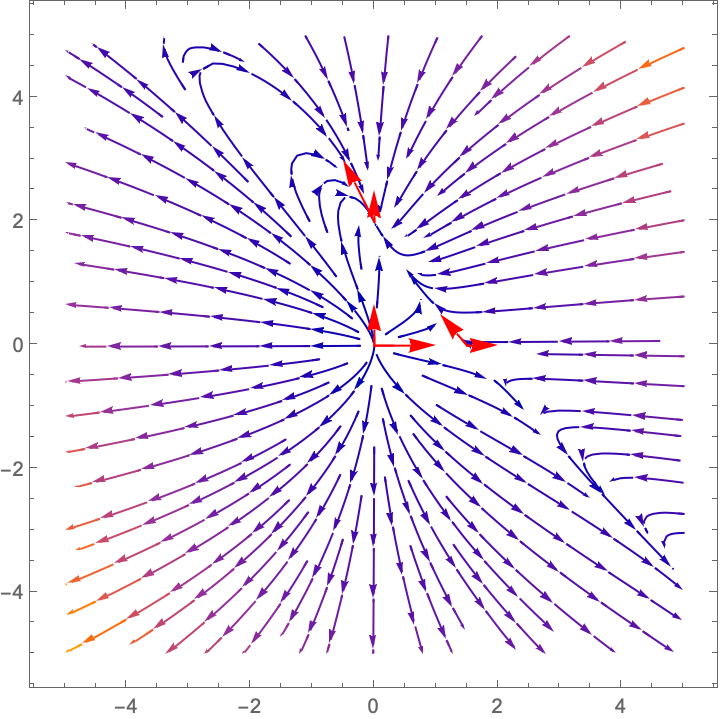
\includegraphics[width=0.4\linewidth]{image.png}
    \caption{Example 1 (from the page before, not the Lorenz System below)}
\end{figure}

\paragraph{Lorenz System}
For first and second order systems, the particle's motion is not chaotic (\url{https://en.wikipedia.org/wiki/Poincar%C3%A9%E2%80%93Bendixson_theorem}). You can predict the particle's behavior: blow up to infinity, go in a loop, go in a limit cycle to approach a cycle, or approach a point. But, in higher order systems, things go crazy sometimes, i.e. the Lorenz system.
\begin{align*}
    \fdiffn{x}{t}=-\sigma x+\sigma y\\
    \fdiffn{y}{t}=\rho x - y - xz\\
    \fdiffn{z}{t} = -\beta z + xy.
\end{align*}
Long term behavior of Lorenz system: two strange attractors
why is it strange?
\begin{enumerate}
    \item Strange geometric properties
    \item Strange mixing properties
\end{enumerate}

\begin{figure}[H]
    \centering
    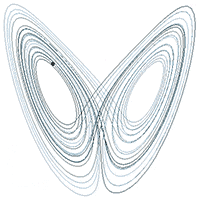
\includegraphics[width=0.25\linewidth]{lorenz.png}
    \caption{Lorenz Attractor}
    \label{fig:enter-label}
\end{figure}

What are these strange geometric properties? Well it turns out that its (Hausdorff) dimension is a non-integer number: specifically around $2.06.$ More generally, fractals have non-integer dimension, such as the Cantor set or the Koch snowflake. A shape is said to have dimension $d$ if its `mass' (area, volume, etc) increases by $2^d$ after scaling up a side length by a factor of 2.

What does it mean to have strange mixing properties? Well, if you start two marbles arbitrarily clos to each other, then after rolling around for long enough, the marbles will be significantly far away. 

The Lorenz equations were intended to simulate atmosphere conditions, and he observered this chaotic behavior through simulations.

\paragraph{Hamiltonian Systems}
Hopping into physics, 
\begin{enumerate}
    \item \[\vec{p}=m\vec{v}.\]
    \[\begin{bmatrix}
        p_1\\p_2\\p_3
    \end{bmatrix}=m\begin{bmatrix}
        v_1\\v_2\\v_3
    \end{bmatrix}.\]
    \[\dot{x_i}=\frac{p_i}{m} \qquad i\in\{1,2,3\}.\]
    \item \[F=\fdiffn{\vec{p}}{t}.\]
    \[\begin{bmatrix}
        F_1\\F_2\\F_3
    \end{bmatrix}=\fdiffn{}{t}\begin{bmatrix}
        p_1\\p_2\\p_3
    \end{bmatrix}.\]
    \[\dot{p_i}=F_i \qquad i\in\{1,2,3\},\]
    \item \[E=K+U,\] where $E$ is total energy, $K$ is kinetic energy, $U$ is potential energy.
    \[\frac{1}{2}m\vec{v}\cdot\vec{v}=\frac{1}{2} m\left[\left(\frac{p_1}{m}\right)^2+\left(\frac{p_2}{m}\right)^2+\left(\frac{p_3}{m}\right)^2\right]=\frac{p_1^2+p_2^2+p_3^2}{m}.\]
    Typically,
    \[U=V(x_1,x_2,x_3),\] for some function $V.$
    \item Total Energy = $H(x_1,x_2,x_3,p_1,p_2,p_3)=V(x_1,x_2,x_3)+\frac{p_1^2+p_2^2+p_3^2}{m}.$
\end{enumerate}
\subsection{More stuff (2.21.2025)}
Remember the Lorenz System, specifically the strange mixing properties, where a small difference in the initial conditions leads to a large difference in the outputs. 

\[H(x_1,x_2,x_3,p_1,p_2,p_3)=V(x_1,x_2,x_3)+\frac{p_1^2+p_2^2+p_3^2}{m}=U+K.\]
\[\fdiffn{K}{p}=\fdiffn{}{mv}\frac{1}{2}mv^2=\frac{1}{2m}\fdiffn{}{v}mv^2 = v,\quad F=\dot p = -\nabla U\]
\[\dot{x_i}=\frac{\partial H}{\partial p_i},\quad\dot{p_i}=-\frac{\partial H}{\partial x_i},\qquad i\in\{1,2,3\},\]

See \url{https://en.wikipedia.org/wiki/Hamiltonian_mechanics#From_Euler%E2%80%93Lagrange_equation_to_Hamilton's_equations}

We have that energy is conserved:
\[\dot{H}=\frac{\partial H}{\partial x}\dot{x}+\frac{\partial H}{\partial p}\dot{p}=\frac{\partial H}{\partial x}\frac{\partial H}{\partial p}+\frac{\partial H}{\partial p}\left(-\frac{\partial H}{\partial x}\right)=0,\]
using multivariable chain rule.

Any (closed) physical system can be written as a Hamiltonian System.

If the system has only one particle, then the dynamics of the system are of order 6 ($x_1,x_2,x_3,p_1,p_2,p_3$), so this particle is in 6-dimensional space. 2 particles live in 12 dimensional space, 3 in 18, etc. $N$ particles are governed by $6n-$order (dimensional) dynamics. In thermodynamics, this kind of thing happens when modeling air in a room, water in a pipe, a rubber band stretching and contracting, with
\[N\sim 10^{23}\text{ to } 10^{25}.\]

How do we visualize a thermodynamic system? Just imagine $10^{23}$ dimensional space! Obviously that is difficult, but since $H$ is conserved, the path of a marble (particle) in phase space is a closed loop (actually a closed $6n-1$ hypersurface). If we put two marbles on this configuration-space loop (hypersurface) arbitrarily close to each other, their true trajectories are unknown, but MUST remain on the loop (hypersurface).

Since we don't know the actual position of a particle, we can just treat the particle like a uniformly distributed probability distribution. Since the consequences of doing this seem to match reality, this is a pretty decent assumption. This connects Shannon entropy $H(X)$ to thermodynamic entropy $S$.

So, how can I model the location of a marble after some time? As a uniform pdf on the level hypersurface. 

Add a differential hypersurface $\Delta H$ to some surface $H.$ If a particle is between $H$ and $H+\Delta H,$ we assume that it will stay in that region over time. So in reality, we lied, it's actually a uniform pdf over the $6N$ dimensional sandwich hypervolume. What does this mean? well we let the differential volume between $\Delta H+H$ and $H$ to be the same locally, so that the surface area is not necessarily the same everywhere; if $\Delta H$ is bigger, the surface area will be smaller to preserve volume. Under this measure, we define our pdf.

\paragraph{Thermodynamic Entropy}
$S(U)$ is Entropy as a function of internal Energy. How do we find $S(U)?$ Well, draw the level hypersurface of 
\[H(x_1,x_2,\dots,p_1,p_2,\dots)=U,\] and then draw the level hypersurface of
\[H(x_1,x_2,\dots,p_1,p_2,\dots)=U+\Delta U,\] where $\Delta U$ is predetermined.
Then consider the volume sandwiched between the two level hypersurfaces. Now, split the sandwich into differential chunks of constant hypervolume $\Delta V.$ The magnitude of the $\Delta V$ (volume not energy) determines the accuracy of the marble's position. The number of chunks is the ratio of the sandwich's volume with $\Delta V$

We define 
\[S(U):=\ln (\#\text{ of chunks}),\] which is just like how the entropy of a uniform (discrete) pdf of $m$ items is $\log_2(m),$ but physicists use $\ln$ because why not.


\paragraph{Properties of $S(U)$}

We don't know the exact form of $S(U),$ because it depends on the specific dynamical system in a high dimension. Nevertheless, it has certain properties:
\begin{enumerate}
    \item $S(U)\ge 0$ because there is at least one chunk.
    \item $S(U)$ is increasing with $U,$ because the level hypersurface $H(\vec{x},\vec{p})=U$ has more hypersurface area as $U$ increases.
    \item $S(U)$ is concave down because $\ln$ is concave down.

    As an example, as the radius of a circle increases, the change in area is
\[\frac{\pi(r+\Delta r)^2-\pi r^2}{\Delta A}\approx 2\pi r\frac{\Delta r}{\Delta A}.\]
If $\frac{\Delta r}{\Delta A}$ is constant, this is linear with $r.$ Basically, it lowers the dimension by 1, so
\[S(U)\approx \log U^{6N-1}=(6N-1)\log U.\]
    \item $S(U)=0$ when $U=0.$ Just trust
    \item $S'(U)=\infty$ when $U=0.$ Also just trust
\end{enumerate}
So, $S$ kinda looks like $\sqrt.$   


\subsection{Legendre Transform (2.25.2025)}
Review: Energy is conserved, so all particles together have a certain amount of energy, and sometime later, they still must have the same energy and must still reside on the level hypersurface $H=U,$ which has dimension $6n-1$ embedded in $6n$-space. Considering the hypersurface $H=U+\Delta U,$ we have a differential hypervolume between these two level surfaces. If a point begins between $H=U$ and $H=U+\Delta U,$ it must stay there forever. Since this dynamical system is chaotic (i.e. we can't determine precisely how the system is truly evolving in time), we can imagine that the time evolution of the phase point as a uniform smeared distribution across the region between $H=U$ and $H=U+\Delta U.$ We can split the hypervolume into $\Delta V$ regions. We assume that $\Delta U$ and $\Delta V$ are given, so we can count the number of chunks of size $\Delta V$ in the region between $H=U$ and $H=U+\Delta U;$ the natural log of this number is entropy.


\paragraph{Another view of $S(U)$}
Remember that
\[H(x_1,x_2,\dots,p_1,p_2,\dots)\] is the Hamiltonian that qualifies our physical system. Remembering MVC, the gradient of a level set is the direction and magnitude of the steepest increase, so if we consider an individual pillar of volume,
\[|\vec\nabla H|=\frac{\Delta U}{\text{``height of pillar''}}\] at each point,
where the height of the pillar is loosely the ratio of the $\Delta V$ to the hypersurface on top of where it resides. We are dividing a $6n$ volume by a $6n-1$ volume, so the height is indeed $1$ dimensional.

Specifically,
\[\text{height of a pillar} = \frac{\Delta V}{A_{\text{pillar base}}},\]
\[\frac{1}{|\vec\nabla H|}=\frac{\Delta V}{\Delta U\cdot A_{\text{base of pillar}}}.\]

Integrate both sides over the level surface $H=U$ using the differential area of the level surface $d\sigma$. \textbf{We fix the location of every pillar ahead of time} such that the integrals below break up into many piecewise integrals (i.e. the integrand is \emph{not} considering continuously trying to place a pillar at every location as grant thought).

\[\int_{\text{level surface}}\frac{1}{|\vec\nabla H|}\diffn{\sigma}=\int_{\text{level surface}}\frac{\Delta V}{\Delta U}\frac{1}{A_{\text{base of pillar}}}\diffn{\sigma}.\]
Just for fun, take the log (remember what we are trying to do: redefine entropy):
\[\ln\int_{\text{level surface}}\frac{1}{|\vec\nabla H|}\diffn{\sigma}=\ln\int_{\text{level surface}}\frac{\Delta V}{\Delta U}\frac{1}{A_{\text{base of pillar}}}\diffn{\sigma}=\ln\frac{\Delta V}{\Delta U}+\ln\int_{\text{level surface}}\frac{1}{A_{\text{base of pillar}}}\diffn{\sigma}.\]

For every patch area, the integral
\[\int_{\text{patch}}\frac{1}{A_{\text{base of pillar}}}\diffn{\sigma}=1,\]
\[\int_{\text{level surface}}\frac{1}{A_{\text{base of pillar}}}\diffn{\sigma}=\sum_{\text{patches}}\int_{\text{patch}}\frac{1}{A_{\text{base of pillar}}}\diffn{\sigma}=\sum_{\text{patches}}1=\# \text{ base patches}.\]
Additionally,
\[\frac{\Delta V}{\Delta U}\] is a constant that is fixed w.r.t $U.$ This may appear to be nonsensical because it $\frac{\Delta V}{\Delta U}$ isn't dimensionless, but we can just normalize by multiplying by a factor (I don't buy this logic but it's fine). So,
\[\ln\int\frac{1}{|\vec\nabla H|}\diffn{\sigma}=\ln(\# \text{ chunks})=S(U),\] up to a constant.

Alternatively:
\[\int\frac{1}{|\vec\nabla H|}\diffn{\sigma}=\int\frac{\text{height of pillar}}{\Delta U}\diffn{\sigma}=\frac{\Delta V}{\Delta U}\int\frac{\text{height of pillar}}{\Delta V}\diffn{\sigma},\] and $S(U)$ follows from taking natural log.

Something something Boltzmann's constant.


\paragraph{Legendre Transform}
This is an important transformation in physics. Consider a function $y(x).$ To specify the curve of the function, we can specify a $y$ coordinate corresponding to every $x$ coordinate.

In another view of the world, we could instead consider every slope of a tangent line ($m$) and correspond it with some number $\beta =f^\ast(m)$ that is the (negative of the) first $y-$intercept of the line that touches the function. Note, this only provides a lower envelope of the function. Specifically:
For every slope $m,$ start with a line of slope $m$ at the very bottom of the cartesian plane. Move this line up until it first touches the curve, and call the negative of the value of the $y$ coordinate $\beta.$

If I have $y=f(x),$ can I find $\beta=f^\ast(m)?$ Yes:
\[f^\ast(m)=\max_{x}[mx-f(x)].\] For every $m,$ we draw a line through the origin with that slope, and then we bring it down by the biggest gap between $mx$ and $f(x),$ and the distance you pull it down is exactly the negative y-intercept $\beta.$ Try to see why this is the same as our previous definition. This only works for convex functions btw, for pretty straightforward reasons (try to do this on $-x^2$ and see what happens).

\paragraph{Example}
\[f(x)=cx^2.\]
For every $m,$ we have $f'(x)=2cx=m,$ so $x=\frac{m}{2c}$ and $cx^2=\frac{m^2}{4c}.$
So,
\[f^\ast(m)=mx-cx^2=\frac{m^2}{2c}-\frac{m^2}{4c}=\frac{m^2}{4c}.\]

\subsection{Legendre Transform 2 Electric Boogaloo (2.27.2025)}
Remember the Legendre Transform:
\[y=f(x)\implies \beta=f^\ast(m),\]
where $f^\ast(m)$ is the negative y-intercept of the lowest line that touches the curve. This is also
\[\max_x[mx-f(x)].\]
\paragraph{Example 1}
\[f(x)=e^x\]
We have
\[f^\ast(m)=\max_x[mx-e^x],\] so $m=e^x,$ or $x=\ln m.$ Plugging this in,
\[f^\ast(m)=m\ln m-m.\]

\paragraph{Example 2}
\[f^\ast(m)=\max_x[mx-x\ln x],\] so $m=\ln x + 1,$ or that $x=e^{m-1}.$ Plugging this in,
\[f^\ast(m)=me^{m-1}-e^{m-1}(m-1)=e^{m-1}.\]
\paragraph{Example 3}
\[f(x)=\begin{cases}
    x^2&2<x<3\\
    \infty &\text{o/w}
\end{cases}.\]
For $4<m<6,$ this is the same as the Legendre Transform of $x^2,$ for which $f^\ast(m)=\frac{m^2}{4}.$ When $m<4,$ the line will go through $(2,4),$ so
\[\frac{4+\beta}{2}=m,\] or
\[\beta=2m-4.\]

For $m>6,$ the line will go through $(3,9),$ so
\[\frac{9+\beta}{3}=m,\] or
\[\beta=3m-9.\]
So
\[f^\ast(m)=\begin{cases}
    2m-4& m<4\\
    \frac{m^2}{4}&4\le m\le 6\\
    3m-9 & m>6
\end{cases}\]

\paragraph{Properties of Legendre Transform}
Assume that the curve is convex.

% https://q.uiver.app/#q=WzAsNCxbMCwwLCJmIl0sWzIsMCwiZl5cXGFzdCJdLFswLDIsImYnIl0sWzIsMiwiKGZeXFxhc3QpJyJdLFsxLDAsIlxcdGV4dHtMLlQufSIsMix7InN0eWxlIjp7InRhaWwiOnsibmFtZSI6ImFycm93aGVhZCJ9fX1dLFsyLDMsIlxcdGV4dHtpbnZ9IiwyLHsic3R5bGUiOnsidGFpbCI6eyJuYW1lIjoiYXJyb3doZWFkIn19fV0sWzEsMywiXFxmcmFje1xcbWF0aHJtIGR9e1xcbWF0aHJtIGR4fSJdLFswLDIsIlxcZnJhY3tcXG1hdGhybSBkfXtcXG1hdGhybSBkeH0iLDJdXQ==
\begin{tikzcd}
	f && {f^\ast} \\
	\\
	{f'} && {(f^\ast)'}
	\arrow["{\frac{\mathrm d}{\mathrm dx}}"', from=1-1, to=3-1]
	\arrow["{\text{L.T.}}"', tail reversed, from=1-3, to=1-1]
	\arrow["{\frac{\mathrm d}{\mathrm dx}}", from=1-3, to=3-3]
	\arrow["{\text{inv}}"', tail reversed, from=3-1, to=3-3]
\end{tikzcd}

\begin{enumerate}
    \item $(f^\ast)^\ast=f.$ 
    \item $(f^\ast)'=(f')^{-1}$
\end{enumerate}
Compactly,
\[\fdiffn{f}{x}=m,\fdiffn{f^\ast}{m}=x,f(x)+f^\ast(m)=mx.\]
Because $f$ is convex,
\begin{align*}
    f^\ast(m)& = \max_x \,mx - f(x) \\
    m &= f'(x), \qquad x = [f']^{-1}(m)  \\
    f^\ast(m) &= m [f']^{-1}(m) - f\circ [f']^{-1}(m)
    \end{align*}
    \begin{align*}
    (f^\ast)'(m) &= [f']^{-1}(m) + m \left(\fdiffn{}{m} [f']^{-1}(m)\right)-f'\circ[f']^{-1}(m)\left(\fdiffn{}{m}[f']^{-1}(m)\right)=[f']^{-1}(m) \\ &\therefore [(f^\ast)']^{-1}(m)=f'(m)\\
    f^{\ast\ast}(m) &= m [(f^\ast)']^{-1}(m) - f^\ast \circ [(f^{\ast})']^{-1}(m) \\
    &= m f'(m) - (mf'(m) - f(m)) \\
    &= f(m).
\end{align*}


\paragraph{2-D Legendre Transform}
Let $y=f(x_1,x_2)$ be a convex surface in $\mathbb{R}^3.$  There are three different ways we could define the Legendre Transform
\begin{enumerate}
    \item Pin down $x_2$ to get a 1-D function $y=f_{x_2}(x_1),$ after which you can take the 1-D Legendre Transform $\beta=f_{x_2}^\ast(m_1),$
    which can be extended to a function of $m_1$ and $x_2:$
    \[\beta=f^\ast(m_1,x_2).\]
    \item Pin down $x_1,$ so that $y=f_{x_1}(x_2),$ and similarly get
    \[\beta=f^\ast(x_1,m_2).\]
    \item Take the true 2-D Legendre Transform. Just like our tangent line, we can take a plane at negative infinity (instead of a line) of slope $\langle m_1,m_2\rangle,$ and bring it up until it touches our surface. Then, we assign $\beta$ to be the negative of the $y$-intercept. Specifically,
    \[\beta=\max_{x_1,x_2}[m_1x_1+m_2x_2-f(x_1,x_2)].\] Using vector notation, where
    \[y=f(\vec{x}):\]
    \[\beta=f^\ast(\vec{m})=\max_{\vec{x}}[\vec{m}\cdot\vec{x}-f(\vec{x})].\]
    \end{enumerate}
\paragraph{Example 4}
\[y=2x_1^2+x_2^2+4.\]
First method: Consider
\[y_{x_1}(x_2).\] We have
\[f^\ast(m_1,x_2)=\max_{x_1}[m_1x_1-2x_1^2-x_2^2-4],\]
so
\[\frac{\partial}{\partial x_1}(m_1x_1-2x_1^2-x_2^2-4)=m_1-4x_1=0,\]
so $x_1=\frac{m_1}{4}.$ Plugging that back in,
\[f^\ast(m_1,x_2)=\frac{m_1^2}{8}-x_2^2-4.\]

Second method:
\[f^\ast(x_1,m_2)=\max_{x_2}[m_2x_2-2x_1^2+x_2^2+4],\]
so
\[\frac{\partial}{\partial x_2}(m_2x_2-2x_1^2-x_2^2-4)=m_2+2x_2=0,\]
so $x_2=\frac{m_2}{2}.$
\[f^\ast(x_1,m_2)=\frac{m_2^2}{4}-2x_1^2-4.\]
    OK so I don't know what happened here because I can't figure out what the original problem is from what I wrote. Sorry, I made a lot of mistakes because class was ending, but I think you get it.
Third method:
\[f^\ast(\vec{m})=\max_{\vec{x}}[\vec{m}\cdot\vec{x}-f(\vec{x})],\]
so this is a stationary point w.r.t. $\vec{x}:$
\[\nabla (\vec{m}\cdot\vec{x}-f(\vec{x}))=\begin{bmatrix}
    m_1-4x_1\\
    m_2+2x_2,
\end{bmatrix}\]
solving for $m_1$ and $m_2,$
\[f^\ast(m_1,m_2)=\frac{m_1^2}{8}+\frac{m_2^2}{4}-4.\]
\subsection{Finishing Legendre Transform 3.3.2027}
\paragraph{2-D Legendre transform}
Let a paragraph have a position $x$ and $p$ travelling in one dimension but existing in $2-d$ phase space.

\[H(x,p)=T+V=\frac{p^2}{2m}+V(x).\]

Take the Legendre Transform of this, only with respect to $p.$

We have
\[H_{x}(p)=\frac{p^2}{2m}+V(x).\] Since we let $m$ denote mass, we will let $v$ denote slope (with no foreshadowing definitely...):
\[v=\frac{\partial}{\partial p}H_x(p)=\frac{p}{m},\] so
\[\mathcal{L}\{H(x,p)\}=vp-\frac{p^2}{2m}-V(x)=\frac{1}{2}mv^2-V(x).\]
This is called the Lagrangian of the particle.

Remember that $S(U)$ is concave down (looks like $\sqrt x$). But, physicists don't like happiness, so they want a convex function. Thus, we define $U(S),$ where energy is a function of entropy. This is helpful because convexity is nice for Legendre transforms.

\paragraph{Temperature}
We define
\[T(S)=\fdiffn{}{S}U(S).\] This clearly is temperature, so I don't see why I should have to explain. Since $U$ is increasing, we have that $T\ge 0$ (in Kelvin). We said that $S$ was a function of one variable, but this can be expanded to $S(U, V_1,V_2,\dots),$ which can be turned into $U(S,V_1,V_2,\dots)=U(S,V).$ Since we are talking about gasses and fluids, we can let $V$ be volume. So,
\[T(S,V)=\frac{\partial}{\partial S}U(S,V).\]
We also have
\[\frac{\partial}{\partial V}U(S,V)=P(S,V),\] pressure as a function of entropy and volume. 

First, let's take the Legendre transform of $U$ w.r.t. $S.$
\[m=\frac{\partial}{\partial S}U(S,V)=T(S,V),\] so we have
\[-U^\ast(T,V)=-\max_S TS-U(S,V)=\inf_S U(S,V)-TS.\]

It turns out that $-U^\ast(T,V)$ is known as the Helmholtz Free Energy.

What about the Legendre transform w.r.t $V?$
Do the same thing, now we have
\[-U^\ast(S, P)=\max_V U(S,V)-PV,\] which is called Enthalpy.

If we take the Legendre Transform w.r.t both, we get Gibbs Free Energy from Chemistry.

\newpage 

\begin{figure}[h!]
    \centering
    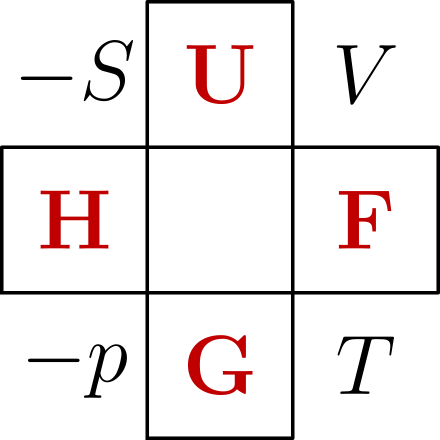
\includegraphics[width=0.2\linewidth]{thermosquare.png}
    \caption{The Thermodynamic Square}
    \label{thermosquare}
\end{figure}

How to read the square?
We have
\[\diffn{U}=-p(\diffn{V})+T(\diffn{S}),\] similarly
\[\diffn{H}=V(\diffn{p})+T(\diffn{S}).\] Why? No idea.


\paragraph{Final Remarks}
Just for fun: \[S(U,V,N),\] where $N$ is the number of moles of particles.
\[\frac{1}{T}=\frac{\partial S}{\partial U},\frac{P}{T}=\frac{\partial S}{\partial V},\frac{\mu}{T}=\frac{\partial S}{\partial N}.\]
We call
$\frac{\mu}{T}$ the chemical potential.

Laws of Thermodynamics.
\begin{enumerate}
    \item \[\Delta S=\frac{\partial S}{\partial U}\Delta U+\frac{\partial S}{\partial V}\Delta V+\frac{\partial S}{\partial N}\Delta N=\frac{1}{T}\Delta U+\frac{P}{T}\Delta V+\frac{\mu}{T}\Delta N.\] We assume that $\Delta N=0$ in a closed system, so
    \[\Delta S=\frac{\Delta U}{T}+\frac{P}{T}\Delta V,\]
    or
    \[T\Delta S=\Delta U+P\Delta V,\Delta U=T\Delta S-P\Delta V.\] If you remember that heat ($Q$) is just $T\Delta S,$ this might make more sense.
    \item Consider an ideal monoatomic gas. Then
    \[S=\frac{3kN}{2}\left[\frac{2}{3}\ln V+\ln U-\frac{5}{3}\ln N\right].\] Sorry, but that's just how it is.
    We have
    \[\frac{\partial S}{\partial U}=\frac{3kN}{2U}=\frac{1}{T}\implies T=\frac{2}{3k}\frac{U}{N}.\]
    \[\frac{\partial S}{\partial V}=\frac{3kN}{2}\frac{2}{3V}=\frac{P}{T}\implies P=\frac{kN T}{V},\] so
    \[PV=kNT.\] Sounds familiar? It's just $PV=nRT.$
    \item Second Law of Thermodynamics
    
    A closed system is in equilibrium iff $S$ is maximized. Let $p$ be the  density at every time, and $q$ be the final equilibrium distribution, for which $S$ is maximized: $q$ is uniform. The second law tells you that
    \[D(p||q)\to 0.\]
\end{enumerate}

\subsection{Finish Thermodynamics (3.5.2025)}
\paragraph{Examples}
\[f(x)=|x|.\]
When $|m|>1,$ we have $f^\ast(m)=\infty$ because we can lower the line forever low while it still hits it.
Otherwise, it hits it at the origin, so $f^\ast(m)=0.$

\[f(x_1,x_2)=|x_1|e^{x_2}.\]

Just like the previous problem,
\[f^\ast(m_1,x_2)=\begin{cases}
    0&|m_1|\le e^{x_2}\\
    \infty & \text{otherwise}
\end{cases}.\]

We have
\[f_{x_1}(x_2)=|x_1|e^{x_2},\] which is convex in $x_2,$ so
\[m_2=\frac{\partial}{\partial x_2}|x_1|e^{x_2}=|x_1|e^{x_2},\] or that
\[x_2=\ln\frac{m}{|x_1|},\] so

\[f^\ast(x_1,m_2)=m_2\ln\frac{m_2}{|x_1|}-m_2\]

For the third way, since this function is convex in $x_1$ and $x_2,$ we have
\[\begin{bmatrix}
    m_1\\m_2
\end{bmatrix}=\nabla f=\begin{bmatrix}
    \Theta(x_1)e^{x_2}\\|x_1|e^{x_2}
\end{bmatrix},\]
where
\[\Theta(x)=\begin{cases}
    -1&x\le 0\\
    1&x>0,
\end{cases}\]
So,
\[x_1=\frac{m_2}{m_1},x_2=\ln(|m_1|).\]
\[f^\ast=m_1x-m_2x-|x_1|e^{x_2}=m_2\ln(|m_1|).\]

\[S=\ln(\text{volume chunks}).\]
$S(U)$ is increasing, concave, derivative of infinity at zero.
But also, $S(U,V)$ or $S(U,V,N)$, but we can make it convex like $U(S,V)$ or $U(S,V,N)$.

\[T=\frac{\partial U}{\partial S},\frac{P}{T}=\frac{\partial S}{\partial V}.\] 

We have (first law)
\[\Delta U=T\Delta S-P\Delta V.\]

Second law:
A system is in equilibrium when $S$ is maximized. 

Consider two chambers of gas separated by a wall. We can assume three possibilities:
\begin{itemize}
    \item Rigid: $V_1,V_2$ are constant
    \item Insulating: $U_1,U_2$ are constant
    \item Impermeable: $N_1,N_2$ are constant
\end{itemize}

First, assume that the wall is rigid and impermeable but non-insulating.
Initial: $S(U_1,V_1,N_1)+S(U_2,V_2,N_2)$
Final: $S(U^\ast_1,V_1,N_1)+S(U^\ast_2,V_2,N_2).$
By conservation of energy,
\[U_1+U_2=U^\ast_1+U^\ast_2.\] The final state will maximize entropy, which we can solve with Lagrange multipliers:
$\mathcal{L}(U^\ast_1,U^\ast_2,\lambda)=S(U^\ast_1,V_1,N_1)+S(U^\ast_2,V_2,N_2)-\lambda(U_1+U_2-U^\ast_1-U^\ast_2).$
Taking partials w.r.t $U^\ast_1,U^\ast_2,$
\[\frac{\partial\mathcal{L}}{\partial U^\ast_1}=\frac{1}{T^\ast_1}-\lambda=0,\qquad\frac{\partial \mathcal{L}}{\partial U^\ast_2}=\frac{1}{T^\ast_2}-\lambda =0,\] so they have the same temperature in equilibrium. We can try the same idea for insulating rooms.

\section{Statistics}
\subsection{Intro/Review to Stats 2025.03.11}
Statistics is a probability `box' run backwards. Usually, we run forward from a known probability model (normal distribution, poisson random variable) to compute data. In statistics, we have the data and predict what's in the box.

Observational vs. experimental studies: actively changing conditions. In experiments, \textbf{random assignment} MUST be used to establish causation, but it is not present in observational studies. 

Let us consider an observational study on a random variable $X$, the flipping of a biased coin with H, T probability $p$, $1-p$. We do not know the value of $p$, which must be determined by observing flips (the sample data of $n$ tosses $x_1,x_2,x_3,\dots,x_n$). Let \[\hat p = \frac{\text{\# of heads}}{n}\] be our estimate of $p$. Here, $\hat p$ itself is a random variable, with $E[\hat p] = p$. We call $\hat p$ a \emph{statistic} because it is based on data, while we call $p$ a \emph{parameter} because it is the truth, based on population. We can also compute error of the mean with
\[\text{Var}[\hat p] = \frac{p(1-p)}{n}.\]
This is derived from the variance of a binomial distribution, $\text{Var}[X] = n p (1-p)$, along with the fact that $\text{Var}[a\cdot X] = a^2 \text{Var}[X]$. The distribution of $\hat p$ is a normal distribution (central limit theorem?), which is completely determined by the mean and variance above.

Statistical \emph{significance} is the surprise factor (like entropy). If the probability of something happening (or of being more extreme) is small, then the result is more surprising/significant/important. Sample size is important for significance.

The \emph{confidence interval} asks how likely it is that the true value $p$ falls within a given interval around $\hat p$. Consider an observed $\hat p = 0.31$ with $n=5046$. We can just say $p\approx \hat p$ and make a normal distribution with $\mu = \hat p$ to compute the confidence interval. With the standard deviation $\sigma$, we compute the confidence interval:
\[\hat p \pm \text{scale factor} \cdot \sqrt{\frac{\hat p (1 - \hat p )}{n}}\]
where the scale factor controls what confidence we want (95\% confidence interval $\approx 2\sigma$. erf!).


\paragraph{Example 2}
Assuming you observe 50 out of 600, what is the chance of seeing $\ge 59$ out of 600 with a new sample? We use the normal distribution's CDF. On TI-84, we have $\text{normalcdf}(\text{lower bound}, \text{upper bound}, \mu, \sigma)$ and $\text{invNorm}(\text{area to the left}) = \text{cdf}^{-1}(\dots)$.

With $\mu = \frac{50}{600}$, $\sigma = \sqrt{\frac{(50/600)(1-50/600)}{600}}$, we have $1-\text{cdf}(59/600) \approx \boxed{9.186\%}$.


\subsection{Experimental Studies (3.13.2025)}
Recall that the 95\% confidence interval of $\hat{p}$ is $\hat p\pm1.96\sqrt{\frac{p(1-p)}{n}}.$ So, 95\% of the time, we can assume that
\[\hat{p}\pm1.96\sqrt{\frac{p(1-p)}{n}}\] contains $p.$ 


There are three kinds of lies: lies, damned lies, and statistics:
\[\hat{p}\pm1.96\sqrt{\frac{\hat{p}(1-\hat{p})}{n}}\] contains $p$ 95\% of the time on average.

Assume that we have a normal distribution $\hat p$ centered at $p_0$ with variance
\[\frac{p_0(1-p_0)}{n}.\] We guess that $p_0$ is the true probability/proportion (null hypothesis). If we measure $p_1,$ then what is the chance that we measure something beyond $p_1$ from $p_0$? This area is the $p$-value. If the $p$-value is small, then the result $p_1$ is significant, so $p_0$ is wrong. If the $p$-value is not small, then we don't know.


For problems 3 and 4, our underlying variable continuous, so we use $\mu$ instead of $p.$

We want to estimate the population mean $\mu,$ which we don't know. All we know are the samples $x_1,x_2,\dots,x_n,$ with a mean $\bar{x}.$ We can't find $\mu,$ but we can get pretty close to it. Our confidence interval is
\[\bar{x}\pm 1.96\frac{\sigma}{\sqrt{n}},\] where $\sigma$ is the population standard deviation. Why? The central limit theorem tells us that $\bar{x}$ is distributed normally, with mean $\mu$ and standard deviation (actually the standard deviation of the mean) is $\frac{\sigma}{\sqrt{n}}.$ Just like before, we guess that $\mu_0$ is the true mean (null hypothesis), and measure $\bar{x}_1,$ and define the $p$-value to be the area further away from $\bar{x}_1.$ If the $p$-value is small enough, we assume that our measured value is significant. But, how would we know $\sigma?$ We don't have the population standard deviation, so we estimate $\sigma$ based on $x_1,\dots,x_n$ to get $s_x.$ This is the sample standard deviation, which we can substitute in for $\sigma$ to get our confidence interval:
\[\bar{x}\pm 1.96\frac{s_x}{\sqrt{n}}.\] But since we use $s_x$ instead of $\sigma,$ it doesn't follow a normal distribution but a $t$-distribution, so we get
\[\bar{x}\pm t^\ast\frac{s_x}{\sqrt{n}}.\] Basically, $t^\ast$ is slightly wider than $1.96.$


Back to Exercise 3:
$\bar{x}=26\si{min}$
Our 95\% confidence interval is
\[26\pm (1.96)\frac{157}{\sqrt{100}},\] and our 99\% confidence interval is \[26\pm2.58\frac{1.57}{\sqrt{100}}.\]

Exercise 4:
\[P(\bar{x}<4.77|\mu=5)=P\left(z<\frac{\bar{x}-\mu}{\sigma/\sqrt{n}}\right)\approx0.18.\]
\subsection{2-Sample (3.17.2025)}
When we have continuous data and we want to determine $\mu,$ we use $\bar{x},$ which is the average of the $x_1,x_2,\dots,x_n,$ and we have our sample standard deviation $s_x.$ Recall that
\[\mathrm{Var}[X]=\mathrm{E}[X^2]-(\mathrm{E}[X])^2=\sum (X-\mu)^2P(X=x).\] Note that to find $\bar{x}$ or $\sigma_x,$ we assume that $x_i$ are uniform, but this isn't exactly right:
\[s_x=\sqrt{\frac{1}{n-1}\sum(x_i-\bar{x})^2}.\] We call $\bar{x}$ an unbiased estimate of $\mu,$ which means that if we plot various $\bar{x},$ we will get a normal distribution centered around $\mu,$ so $\bar{x}$ is directly correlated to $\mu.$ For this to be true, we must use $n-1$ in the denominator instead of $n.$ Why? If we have $\bar{x}$ fixed, then the first $n-1$ $x_i$'s determine $x_n,$ so we only have $n-1$ degrees of freedom (Bessel's correction).

\paragraph{2-Sample}
When we have a 2-sample test, we want to compare two samples (no kidding), but we have two parameters that we want to estimate, $p_1$ and $p_2.$ But, we can reduce this to a one parameter situation. If $p_1$ is the proportion of teen drivers ignoring cell phone bans before 2006 and $p_2$ is the proportion after the date, we only really care about $p_1-p_2$ to see if there is a difference between the data, making this a one-parameter test. If we consider the difference $\hat p_1-\hat p_2,$ since $\hat p_1$ and $\hat p_2$ are normally distributed and independently, we must have that the difference is also normally distributed (\url{https://en.wikipedia.org/wiki/Sum_of_normally_distributed_random_variables}).
The mean of $\hat p_1-\hat p_2$ is $p_1-p_2$ and the standard deviation is $\sigma=\sqrt{\frac{p_1(1-p_1)}{n_1}+\frac{p_2(1-p_2)}{n_2}}.$

For two continuous distributions, we have our confidence interval
\[\bar{x}_1-\bar{x}_2\pm\text{scale factor}\sqrt{\frac{s_{x_1}^2}{n_1}+\frac{s_{x_2}^2}{n_2}}.\] Remember that $s_x$ has the $n-1.$

\subsection{Information Theory Finally (sorry next time) (3.19.2025)}
\subsubsection{Bivariate Data}
Consider data $\langle x_i,y_i\rangle,$ where $x$ and $y$ are discrete random variables, or $x$ is discrete and $y$ is continuous, or $x$ is continuous and $y$ is discrete, or $x$ and $y$ are both continuous. If both are continuous, then we can consider linear regression.
If we have $n$ data points, we can visualize them with a scatterplot of the points $x_i,y_i.$ We want to find the relationship between $x$ and $y,$ and the easiest model to try is a linear model with the lowest rms error (\textbf{vertical} from points to the line). We call $y-\hat{y}$ the residuals. The line $\hat y=a+bx$ that we say is the best model is the one that minimizes the sum of the square of the residuals. It turns out that the line will go through the point $(\bar{x},\bar{y}).$ Consider the following:
\[s_x^2=\frac{1}{n-1}\sum(x_i-\bar{x})^2\qquad s_y^2=\frac{1}{n-1}\sum (y_i-\bar{y})^2.\] Rearranging,
\[\frac{1}{n-1}\sum\left(\frac{x_i-\bar{x}}{s_x}\right)^2=1\qquad \frac{1}{n-1}\sum \left(\frac{y_i-\bar{y}}{s_y}\right)^2=1.\]
We can define the correlation:
\[r_{xy}=\frac{1}{n-1}\sum\left(\frac{x_i-\bar{x}}{s_x}\right)\left(\frac{y_i-\bar{y}}{s_y}\right).\] It turns out that $-1\le r\le 1.$ If $|r|\approx 0.8$ or $0.9,$ then we say there's a strong correlation, but if it's around $0.5,$ then there's a weak correlation. Note that $r$ doesn't depend on which variable we choose to be $x$ or $y,$ nor does it depend on the units of $x$ or $y.$ The value of $r$ corresponds to the strength of the linear relationship between $x$ and $y.$ If $r$ is small, that only means that the linear model is weak, NOT that there is no relationship between $x$ and $y.$ We call $r^2$ the coefficient of determination. This is the proportion of the variation in $y$ that can be attributed to a linear relationship. If $r=0.75,$ then $56.25\%$ of the variation in $y$ can be attributed to a linear relationship between $y$ and $x.$ Specifically, we can define the measure of total variation to be
\[SST=\sum (y_i-\bar{y})^2,\] and
\[SSR=\sum(y_i-\hat y)^2\] is the measure of variation unexplained by the linear model. The ratio between these two terms is $1-r^2:$
\[r^2=1-\frac{\sum(y_i-\hat y)^2}{\sum(y_i-\bar{y})^2}=1-\frac{SSR}{SST},\] only for the best fit line.

Note that, however, if we sample a data set multiple times, we might get a different regression line every time. Instead of a model $\hat y ax+b,$ we can consider the random variable $y$ to be $y=\alpha +\beta x+\varepsilon,$ where $\varepsilon$ is a random variable that represents the residuals. Every time we sample the data, we will get a different value of $\epsilon$ at each point, so it makes sense for this to be a random variable. Furthermore, we can assume that $\varepsilon$ has a normal distribution with zero mean and some $\sigma_\varepsilon$ standard deviation. We also assume that for any fixed value of $x,$ $\varepsilon$ is identically distributed, and so $y$ is normally distributed with mean $\alpha +\beta x$ and stdev $\sigma_\varepsilon.$
\paragraph{Inference}
We can infer things with either a confidence interval (statistic $\pm$ confidence level or scale factor $\times$ stdev of statistic). We are creating a sampling distribution of $b,$ which is a normal distribution with center $\beta$ and standard deviation $\frac{\sigma_\varepsilon}{\sqrt{s_x}}.$ We get $b\pm \frac{\sigma}{\sqrt{s_x}},$ where $\sigma$ is an unknown estimate given our data set. To find $\sigma,$ we use the standard error of the residuals:
\[s_e=\sqrt{\frac{SSR}{n-2}}.\]

\paragraph{Hypothesis Testing}
Given a guess $\beta_0,$ we construct a normal distribution around it and check if $b_0$ is in the confidence interval.
\subsection{Now We Are Doing Info Theory}
\subsubsection{Observational Studies}
Remember what this is: we aren't comparing an input to an output but instead observing the data directly, such as compiling data from a survey. Given a source $Q$ and (list of) observation(s) $\vec{x},$  we want to define some notion of how ridiculous $\vec{x}$ is to come from $Q.$ It's not good enough to use $\text{Prob}_Q(\vec{x})$ as a metric. For example, a biased coin with $p=0.7.$ If we toss it a thousand times, we expect around $700$ heads and $300$ tails. But, the chance of getting a specific $\vec{x}$ is really low, so this isn't a good metric.

Instead, we want $\text{Prob}_Q(\vec{x}\text{ and its entire tail}).$ For every $\vec{x},$ define
\[S_{\vec{x}}=\{\vec{x}'|\text{Prob}_Q(\vec{x}')\le \text{Prob}_Q(\vec{x})\}.\] We call $\vec{x}$ too ridiculous if $\text{Prob}_Q (S_{\vec{x}})$ is small.

Given an $\vec{x},$ find all the $Q$ that might have produced it. We define the Confidence Region to be the set
\[\{Q|\vec{x}\text{ is not ridiculous to have come from }Q\}.\]

\subsubsection{Hypothesis Testing}
Given a $Q$ that Mr. Null guesses, we find all the $\vec{x}$ that will allow you to disprove $Q$ (would be too ridiculous). We define the rejection region to be
\[\{\vec{x}|\vec{x}\text{ is too ridiculous to have come from } Q\}\]

Now we will define $P_Q(\vec{x}).$ We can construct a bar graph that relates possible values $\xi_i$ to an $N_i$ that represents the number of times that $\xi_i$ occurs in $\vec{x},$ such that $\sum_i N_i=N,$ which is the size of $\vec{x}.$
\[P_Q(\vec{x})=\prod_i P_Q(x_i)=\prod_i P_Q(\xi_i)^{N_i}=2^{-\left[\sum_i N_i\log\frac{1}{P_Q(\xi_i)}\right]}=2^{-N\left[P_{\vec{x}}(\xi_i)\log\frac{1}{P_Q(\xi_i)}\right]}=2^{-N[D(P_{\vec{x}}||Q)+H(P_{\vec{x}})]}.\] The numerator term is $N$ times cross-entropy if you know that.

We have
\[\frac{1}{N}\log \frac{1}{P_Q(\vec{x})}\] is basically our average surprise per observation.

Now, we want to find the probability 
\[P_Q(S_{\vec{x}}).\] We can't find this directly but we can bound it, which we need the Pythagorean Inequality for. 

Consider a convex set $S$ of distributions, meaning that any convex combination of distributions in $S$ is also in $S.$ For example, if the distributions $P_1=400H/650T$ and $P_2=450H/550T$ are both in $S,$ then a combination \[pP_1+(1-p)P_2\] is also in $S,$ where $0\le p\le 1.$ \url{https://en.wikipedia.org/wiki/Convex_combination}.

If $S$ is ridiculous, then $Q$ is outside $P.$ If $P^\ast$ is closest to $Q$ (under the K.L. ``metric'', which is not symmetric!), which would be on the boundary of $S$ we have the Pythagorean Inequality (beware that this is backwards from the triangle inequality):
\[D(P||Q)\ge D(P||P^\ast)+D(P^\ast||Q).\]
\paragraph{Proof of Pythagorean Inequality}
Consider some $P_\lambda$ in $S$ such that
\[P_\lambda=\lambda P+(1-\lambda)P^\ast,\] with $0\le\lambda\le 1.$ In the path $P^\ast\leftrightarrow P,$ we have that $D(P^\ast||Q)$ is a minimum of $D(P_\lambda||Q)$ by construction. We get that the derivative of $D(P_\lambda||Q)$ w.r.t $\lambda$ is non-negative at $\lambda=0$. Why? We don't know for sure if $D(P_\lambda||Q)$ is decreasing throughout the entire path, but for sure when we begin leaving the minimum near $\lambda = 0$, we must have $D(P_\lambda||Q)$ is increasing, because otherwise some other point must be the minimum (violating our definition of $P^\ast$).

\[D(P_{\lambda}||Q)=\sum P_{\lambda}\log\frac{P_{\lambda}}{Q}\]
\begin{align*}\left.\fdiffn{D}{\lambda} \right|_{\lambda=0}&=\sum\left[(P-P^\ast)\log\frac{P_\lambda}{Q}+(P-P^\ast)\right]\\&=\sum(P-P^\ast)\log\frac{P^\ast}{Q}+0\\&=\sum P\log \frac{P^\ast}{Q}-\sum P^\ast \log \frac{P^\ast}{Q}\\&=\sum P\log\left[\frac{P}{Q}\cdot\frac{P^\ast}{P}\right]-\sum P^\ast\log\frac{P^\ast}{Q}\\&=D(P||Q)-D(P||P^\ast)-D(P^\ast||Q)\ge 0,\end{align*}
so
\[D(P||Q)\ge D(P||P^\ast)+D(P^\ast||Q).\]

This might make some intuitive sense because you can consider the triangle connecting $P,P^\ast,Q$ which must be obtuse because our set is convex. So, we might expect something like \[(PP^\ast)^2+(P^\ast Q)^2\le (PQ)^2,\] which is similar to what we have.
\subsection{Information Theory (Observational Studies).}
Remember that
\[P_Q(S)=\sum_{\vec{x}\in S}P_Q(\vec{x})=\sum_{\vec{x}\in S}2^{-N[D(P_{\vec{x}}||Q)+H(P_{\vec{x}})]}.\]
By Pythagoras:
\begin{align*}P_Q(S)&\le\sum_{\vec{x}\in S}2^{-N[D(P_{\vec{x}}||P^\ast)+D(P^\ast||Q)+H(P_{\vec{x}})]}\\&=2^{-ND(P^\ast||Q)}\sum 2^{-N[D(P_{\vec{x}}||P^\ast)+H(P_{\vec{x}})]}\\&=2^{-ND(P^\ast||Q)}P_{P^{\ast}}(S).\end{align*}
And, since probabilities are $\le$ 1, we have
\[P_Q(S)\le 2^{-ND(P^\ast||Q)}.\]

\paragraph{Some Handy Formulas}
KL Divergence between two bernoulli distributions:
\[D(Bernoulli(p_1)||Bernoulli(p_2))=p_1\log\frac{p_1}{p_2}+(1-p_1)\log \frac{(1-p_1)}{(1-p_2)}=\frac{1}{\ln 2}\left[p_1\ln\frac{p_1}{p_2}+(1-p_1)\ln\frac{1-p_1}{1-p_2}\right].\]

Remember that \[\ln(1+\varepsilon)\approx \varepsilon-\frac{\varepsilon^2}{2},\] and we can assume that $p_1$ is close to $p_2:$
\[D\approx \frac{1}{2\ln 2}\frac{(p_1-p_2)^2}{(p_1)(1-p_1)}\] apparently.

Apparently, you can do the same thing for two Gaussians (using integrals instead of sums), you get
\[D[N(\mu_1,\sigma_1)||N(\mu_2,\sigma_2)],\] and if $\sigma_1=\sigma_2=\sigma,$
then
\[D\approx\frac{1}{2\ln 2}\frac{(\mu_1-\mu_2)^2}{\sigma^2}.\] If $\mu_1=\mu_2,$ $D=0,$ so this is reasonable.

\paragraph{Observational Study for Proportions}
Remember that our confidence interval is \[\hat{p}\pm C\sqrt{\frac{\hat p(1-\hat p)}{n}}.\] Assume that we observe $\vec{x}=x_1,x_2,\dots,x_N$ from a $Bernoulli(p),$ which is our $Q,$ making it a binomial distribution since we repeat it $N$ times. If $\vec{x}$ is too ridiculous to have come from $Q,$ then
\[P_Q(S_{\vec{x}})\le2^{-ND(P^\ast||Q)}<\varepsilon\] for some small $\varepsilon.$ It turns out that our $P^\ast$ is $Binomial(\hat p).$ This is the closest distribution in $S(\vec{x})$ to $Q.$

We can calculate
\[2^{-N D(P^\ast||Q)}\approx 2^{-N\left[\frac{1}{2\ln 2}\frac{(\hat p-p)^2}{\hat p(1-\hat p)}\right]}<\varepsilon,\] so
\[\frac{1}{2\ln 2}\frac{(\hat p-p)^2}{\frac{(\hat p)(1-\hat p)}{N}}>\log\frac{1}{\varepsilon},\] so
\[\frac{(\hat p-p)^2}{\frac{\hat p(1-\hat p)}{N}}>\ln\frac{1}{\varepsilon^2},\]
so
\[\frac{|\hat p-p|}{\sqrt{\frac{\hat p(1-\hat p)}{N}}}>\sqrt{\ln\frac{1}{\varepsilon^2}}=C,\] our scaling factor. So, our confidence interval is an $p$ such that
\[\frac{|\hat p-p|}{\sqrt{\frac{\hat p(1-\hat p)}{N}}}\le C.\] In other words, $\hat p\pm C\sqrt{\frac{\hat p(1-\hat p)}{N}}$ contains $p.$ If $\varepsilon=0.05$ (95\% confidence interval), we get $C\approx 2.45,$ which is a wider interval that our $1.96$ scale factor interval, but not that bad.

We can do the exact same thing with normal distributions, where $Q\sim N(\mu,\sigma)$ creates observed $x_1,x_2,\dots,x_N,$ so that
\[P^\ast\sim N(\bar{x},s_x).\] Repeating the same idea, we get the confidence interval to be the set of $\mu$ such that
\[\frac{|\bar{x}-\mu|}{s_x/\sqrt{N}}\le C,\] or \[\bar{x}\pm C\frac{s_x}{\sqrt{N}}.\]

\subsection{idk what we are doing today (3.27.2025)}
\subsubsection{Observational Studies}
Remember last time we were trying to tie in $2^{-ND(P^\ast||Q)}$ with formulas. We defined that the confidence interval is
\[\left\{p\Bigg\vert\frac{|\hat p-p|}{\sqrt{\frac{\hat p(1-\hat p)}{N}}}\le C\right\}.\]
For our hypothesis testing, our rejection region given a $p$ is the set
\[\left\{\vec{x}\Bigg\vert\frac{|\hat p-p|}{\sqrt{\frac{\hat p(1-\hat p)}{N}}}>C\right\}.\]


Similarly for means (continuous):
Confidence interval given $\vec{x}$:
\[\left\{\mu\Bigg\vert\frac{\bar{x}-\mu}{\frac{s_x}{\sqrt{N}}}\le C\right\},\]
Rejection interval given $\mu$:
\[\left\{\vec{x}\Bigg\vert\frac{\bar{x}-\mu}{\frac{s_x}{\sqrt{N}}}>C\right\}.\]

\paragraph{Example}
Assume we have a thousand coin tosses, with a true distribution of $P_h=P_t=0.5.$ We want to find the probability of seeing more than 700 heads or more than 700 tails if I toss the coin a thousand times. We can find $D(P^\ast||Q),$ where $\hat{p}=0.7,$ so
\[D(P^\ast||Q)=0.7\log\frac{0.7}{0.5}+0.3\log\frac{0.3}{0.5}\approx 0.1187.\]
So, we have
\[P(S)=2^{-1000(0.1187)}\approx 10^{-36}.\] Which is really really small.
\subsubsection{Experimental Studies}
We can imagine an experimental study as a channel that turns $x_1,x_2,\dots,x_N$ into $y_1,y_2,\dots,y_N,$ for different inputs $x_i.$ There is some probability $Q(y|x)$ for each $y$ and $x$ that we don't know.

For an observational study, we measure the output $\vec{x}$ of an independent source $Q,$ but now we have an input $\vec{x}$ and we want to figure out what $\vec{y}$ would be too ridiculous to come out of $Q.$ If you have observed $\langle\vec{x},\vec{y}\rangle,$ your best guess for $Q$ is the confidence region:
\[\{Q|\vec{x} \text{ goes into } Q,\vec{y}\text{ is not too ridiculous to observe}\}.\]

If you have a guess for $Q,$ you want to disprove it, which you can do with the hypothesis rejection region:
\[\{\langle\vec{x},\vec{y}\rangle|\vec{x}\text{ into }Q,\vec{y}\text{ is too ridiculous to observe from }Q\}.\]

If we have some $\vec{x}=\langle x_1,x_2,\dots,x_N\rangle,$ we have the possible treatments $\xi_1,\xi_2,\dots,\xi_k.$ For example, if we have 153 patients, then $N=153.$ if we have three different treatments (Advil/Tylenol/Placebo), then $k=3.$ We can decide which $\xi_i$ the $x_j$ go into. We segregate our output ($\vec{y}$) according to the $\xi_1,\xi_2,\dots,\xi_k,$ so that we have $\vec{y_{\xi_1}},\vec{y_{\xi_2}},\dots,\vec{y_{\xi_k}},$ which are the components of $\vec{y}$ whose corresponding components of $\vec{x}$ have a value (treatment) of $\xi_1.$ We can split our distribution $Q(y|x)$ into $Q_{\xi_i}(y)=Q(y|x\text{ took the treatment } \xi_i).$ This gives us $k$ different histograms $Q_{\xi_i}(y),$ which we can treat separately like we did before. 

If the histogram of our observed data $\vec{y_{\xi_1}}$ is ``too different'' from our true distribution $Q_{\xi_1},$ then at least part of the data is ridiculous:
\[2^{-N_1D(P_{\vec{y}_{\xi_1}}||Q)}\le\varepsilon.\] We can do this separately for each $\xi_i,$ but we want to somehow combine them, since one part could be ridiculous when the other isn't. We wish to blend all the decisions from the buckets:
\[\sqrt[^k]{2^{-N_1D(P_{y_{\xi_1}}||Q_{\xi_1})}\cdot2^{-N_2D(P_{y_{\xi_2}}||Q_{\xi_2})}\dots2^{-N_kD(P_{y_{\xi_k}}||Q_{\xi_k})}}\le \varepsilon.\]

We might have have ``Two Proportion'' Situation, where the two input possibilities of $\vec{x}$ are $\xi_1,\xi_2,$ e.g. drug or placebo, and only two output values of $\vec{y}$ can be taken up, e.g. live or die. So, we have that $Q(y|x)$ can be split into two binomials: $Q_{\xi_1}(y)\sim Binomial(p_1),Q_{\xi_2}(y)\sim Binomial(p_2).$ Applying necessary approximations to our expression above, we have
\[\frac{(\hat p_1-p_1)^2}{\frac{\hat p_1(1-\hat p_1)}{N_1}}+\frac{(\hat p_2-p_2)^2}{\frac{\hat p_2(1-\hat p_2)}{N_2}}>\ln \frac{1}{\varepsilon},\] for our ``too ridiculous'' region. Dividing through, we have
\[\frac{(\hat p_1-p_1)^2}{\ln\left(\frac{1}{\varepsilon^2}\right)\frac{\hat p_1(1-\hat p_1)}{N_1}}+\frac{(\hat p_2-p_2)^2}{\ln\left(\frac{1}{\varepsilon^2}\right)\frac{\hat p_2(1-\hat p_2)}{N_2}}>1,\] which is suspiciously like the equation for an ellipse centered at $(\hat p_1,\hat p_2)$ with respect to $p_1$ and $p_2.$ We get that the confidence region is
\[\left\{\langle p_1,p_2\rangle\Bigg\vert\frac{(\hat p_1-p_1)^2}{\ln\left(\frac{1}{\varepsilon^2}\right)\frac{\hat p_1(1-\hat p_1)}{N_1}}+\frac{(\hat p_2-p_2)^2}{\ln\left(\frac{1}{\varepsilon^2}\right)\frac{\hat p_2(1-\hat p_2)}{N_2}}\le 1\right\},\] which is the area inside the ellipse, and our hypothesis rejection region is the area outside the ellipse. In order to make this a single-variate distribution, we look at lines of the form $p_1-p_2=k$ over $k,$ and the confidence interval is the values of $k$ that intersect the ellipse, corresponding to the greatest and least difference in the means.

We could also have a two mean study, where $y_i$ can assume continuous real numbers, such as the number of pounds lost after taking a drug (don't do ozempic guys it's not good for your health). In this case, we have $Q_{\xi_1}(y)\sim N(\mu_1,\sigma_1),Q_{\xi_2}(y)\sim N(\mu_2,\sigma_2).$

\subsection{Finishing Statistics and ... (04.07.2025)}
Recall the two-sample (two-proportion) problem. We have that our rejection region is
\[\frac{(\hat p_1-p_1)^2}{\frac{\hat p_1(1-\hat p_1)}{N_1}}+\frac{(\hat p_2-p_2)^2}{\frac{\hat p_2(1-\hat p_2)}{N_2}}>\ln \frac{1}{\varepsilon},\]
and so 
\[\frac{(\hat p_1-p_1)^2}{\ln\left(\frac{1}{\varepsilon^2}\right)\frac{\hat p_1(1-\hat p_1)}{N_1}}+\frac{(\hat p_2-p_2)^2}{\ln\left(\frac{1}{\varepsilon^2}\right)\frac{\hat p_2(1-\hat p_2)}{N_2}}>1.\]

So, our confidence region is the set
\[\left\{\langle p_1,p_2\rangle\Bigg\vert\frac{(\hat p_1-p_1)^2}{\ln\left(\frac{1}{\varepsilon^2}\right)\frac{\hat p_1(1-\hat p_1)}{N_1}}+\frac{(\hat p_2-p_2)^2}{\ln\left(\frac{1}{\varepsilon^2}\right)\frac{\hat p_2(1-\hat p_2)}{N_2}}\le 1\right\},\] and ellipse.
Our hypothesis rejection region given $\langle p_1,p_2\rangle$ is
\[\left\{\langle\vec{x},\vec{y}\rangle\bigg|\frac{(x-a)^2}{\alpha^2}+\frac{(y-b)^2}{\beta^2}>1 \right\},\] for the proper $\alpha,\beta.$ To make this univariate, we can slide a line ($y-x=k$) across the ellipse instead. Consider the following ellipse:
\[\frac{(x-a)^2}{\alpha^2}+\frac{(y-b)^2}{\beta^2}=1.\] Implicitly differentiating:
\[\frac{2(x-a)}{\alpha^2}+\fdiffn{y}{x}\frac{2(y-b)}{\beta^2}=0,\] so
\[\fdiffn{y}{x}=-\frac{\beta^2(x-a)}{\alpha^2(y-b)}=1,\] so
\[y=b+\frac{\beta^2(x-a)}{\alpha^2}.\] Plugging it back into the ellipse,
\[\frac{(x-a)^2}{\alpha^2}+\frac{\beta^4(x-a)^2}{\alpha^4}\frac{1}{\beta^2}=1,\] so
\[(x-a)^2=\frac{\alpha^4}{\alpha^2+\beta^2},\] and by symmetry,
\[(y-b)^2=\frac{\beta^4}{\alpha^2+\beta^2}.\]
We have
\[x=a\pm\sqrt{\frac{\alpha^4}{\alpha^2+\beta^2}},y=b\pm\sqrt{\frac{\beta^4}{\alpha^2+\beta^2}},\] so the max and min values of $x-y$ are
\[c_1=(a-b)+\sqrt{\frac{\alpha^4}{\alpha^2+\beta^2}}+\sqrt{\frac{\beta^4}{\alpha^2+\beta^2}},c_2=(a-b)-\sqrt{\frac{\alpha^4}{\alpha^2+\beta^2}}-\sqrt{\frac{\beta^4}{\alpha^2+\beta^2}}.\]
And,
\[c_1-c_2=2\sqrt{\beta^2+\alpha^2}=2\sqrt{\frac{\hat p_1(1-\hat p_1)}{N_1}+\frac{\hat p_2(1-\hat p_2)}{N_2}},\] ignoring $\varepsilon$ for now.
So, our confidence interval is $(\hat p_1-\hat p_2)\pm\frac{c_1-c_2}{2}=(\hat p_1-\hat p_2)\pm\sqrt{\frac{\hat p_1(1-\hat p_1)}{N_1}+\frac{\hat p_2(1-\hat p_2)}{N_2}}.$ Adding the $\varepsilon$ term adds a scale factor to our confidence interval but that's too messy here.
\subsubsection{Preview to Kolmogorov Complexity}
Kolmogorov focused on algorithmic information theory, which isn't very practical and very theoretical. Kolmogorov studied the idea of algorithmic complexity, which can be combined with Shannon's ideas of entropy and information.
\section{Kolmogorov Complexity}
\subsection{Introduction to K.C.}
We can consider a process as some machinery that creates data, which we want to find out. But we can see this process the other way, as shown:
\begin{enumerate}
    \item Forward: Given a machinery, determine the data output
    \item Backwards: \begin{enumerate}
        \item Given an observed data, guess which machinery would have generated the data
        \item Given data that you want to create, try to design machinery that would produce it
    \end{enumerate}
\end{enumerate}
For example, we have probability (forward) and statistics (backwards), ML Inference (forward) and ML Learning (backwards), deduction (forward) and induction (backwards), analysis (forward) and synthesis (backwards) etc.

Mathematics can describe data pretty well (like vectors, etc.), but it's difficult to describe machinery. But, with the advent of computer science, we can describe machinery with code or a program. Kolmogorov (20th century) was a superstar in mathematics during the time when computer science was beginning to gain traction (around the time of Turing). Kolmogorov was interested in the backwards program in terms of computer programs that create data. There were two problems:
\begin{enumerate}
    \item Given a Turing machine, find the output
    \item Given data, find the Turing machine that would produce data
\end{enumerate}
The first one is pretty simple since you can just run it, so we will focus on the second one.

\paragraph{Turing Machines}
Primitive programming language, where a program is specified by
\begin{enumerate}
    \item Finite set of states: $Q=\{q_0,q_1,\dots,q_n\}$
    \item Table: $Q\times\{0,1,\text{blank}\}\to Q\times\{0,1,\text{blank}\}\times\{\text{L},\text{R},\text{halt}\}.$
\end{enumerate}

\newpage
\begin{figure}[h!]
\centering
\begin{tabular}{c|c||c|c|c}
\hline
$q_0$&blank&$q_1$&1&R\\
$q_0$&0&$q_1$&0&halt\\
$q_0$&1&$q_1$&1&halt\\
\hline
$q_1$&blank&$q_2$&1&R\\
$q_1$&0&$q_2$&0&halt\\
$q_1$&1&$q_2$&1&halt\\
\hline
$\dots$&$\dots$&$\dots$&$\dots$&$\dots$\\
\hline
$q_{n-1}$&blank&$q_0$&1&halt\\
$q_{n-1}$&0&$q_0$&0&halt\\
$q_{n-1}$&1&$q_0$&1&halt\\
\end{tabular}
\caption{Example Turing Machine}
\end{figure}

So, we start on the left, which is blank, so we place a $1$ and the move right. This is blank, so we place a 1 and move right. Repeating this, we will produce all 1's and then halt. Each Turing machine requires a unique table.

Let us have some program (table) $p$ with length $\ell(p),$ which is the number of bits it takes to write the table. We call $U(p)$ the output on the tape when you run the program (and halts), otherwise we call $U(p)$ undefined.    

There are many programs that will produce the same $U(p)$, and Kolmogorov wants the simplest one (smallest $\ell(p)$). The reverse problem is Busy Beaver (largest $U(p)$ given $\ell(p)$).
Occam's Razor: My car has a flat tire. Either, there's a nail in my tire or someone slashed it. Assume it's the nail. You failed a test. Either you didn't study hard enough or your teacher sabotaged your grade. Obviously the latter.

Basically, choose the simplest model that works. Consider some $X\sim p(X).$ This has descriptive length $\left\lceil\log\frac{1}{p(X=x)}\right\rceil$ Kolgomorov defined algorithmic complexity to be the length of the shortest binary computer program that describes the object. Depending on the program, we might be off by a constant, which is negligible. 
\paragraph{Example 1}
Assume we want the output $0101\dots01$ that has length $2n.$ The easiest way to implement this is with a for loop which has around $\log n$ states (I think, not sure).
\paragraph{Example 2}
$01101010000010011110011001100111111100111\dots$
This looks random, but obviously it's just the binary representation of $\sqrt{2}-1.$
\paragraph{Example 3}
$11011110011101011111110110111110111010110$
Even if there isn't a pattern, we can just print it out!! This means that it will take $n$ bits to describe.

\paragraph{Kolmogorov Complexity}
$x$ is a finite length binary string, $U$ is a universal computer, and $\ell(x)$ denotes the length of the string $x.$ We define the Kolmogorov complexity of $x$ to be
\[\mathcal{K}_U(x)=\min_{p:U(p)=x}\ell(p).\]

\subsection{Kolmogorov Complexity Continued (04.15.2025)}
\[\mathcal{K}_U(x)=\min_{p:U(p)=x}\ell(p).\]
\paragraph{Theorem 1} Universality of K.C.

If $U$ is a universal computer, then for any other computer $A,$ we have $\mathcal{K}_U(x)=\mathcal{K}_A(x)+c_A,$
for strings $x\in\{0,1\}^n$ and $c_A$ is constant w.r.t. $x.$

Proof:
We have a program $p_A$ for a computer $A$ to print some $x,$ so $A(p_A)=x.$ We can precede this with a simulations program $s_A$ which tells computer $U$ to act like computer $A.$ Then, $U$ can interpret the program for $A,$ perform the calculations, and print $x.$ The program for $U$ is thus $p=s_Ap_A$ (concatenation), with length $\ell(p)=\ell(s_A)+\ell(p_A)=c_A+\ell(p_A).$ Then,
\[\mathcal{K}_U(x)=\min\ell(p)\le\min_{A(p)=x}(\ell(p)+c_A)=\mathcal{K}_A(x)+c_A.\] Don't worry too much about $\le$ vs $=,$ since for long enough strings $x,$ we can neglect the $c_A.$ In other words, the K.C. doesn't depend on what computer we use.
\paragraph{Theorem 2} Bounds on K.C.
If we don't know $\ell(x),$ we don't know where to stop, so we need more information to know when to stop printing.
\[\mathcal{K}(x)\le\mathcal{K}(x\mid\ell(x))+\log\ell(x)+c.\] Basically, it takes the length of the program given how long it is along with how long the string is to describe it. For example, if we want to print $100!,$ we don't know the $K$ of the computer to describe it. But, once we tell it that it's 525, then we can describe the output with the number 525 (encoded with at most $\log 525$ bits, although it could be shorter), along with $\mathcal{K}(100!|\ell(100!)=525),$ which is the K.C. given that the output has a length of 525.
\paragraph{Theorem 3}
The number of strings $x$ with complexity $K(x)<k$ satisfies
\[|\{x\in\{0,1\}^\ast:\mathcal{K}(x)<k\}|<2^k,\] where $\{0,1\}^\ast$ is Kleene closure. This is true because $2^0+2^1+2^2+\dots+2^{k-1}=2^k-1,$ which is the possible strings of length less than $k.$


\paragraph{Moving on}
Remember binary entropy $H_2(p)=-p\log p-(1-p)\log(1-p).$ Let $x_i$ be i.i.d. bernoullis, so $\bar{x}=\frac{1}{n}\sum x_i,$ and we define
\[H_2\left(\frac{1}{n}\sum x_i\right)=-\bar{x}_n\log\bar{x}_n-(1-\bar{x}_n)\log(1-\bar{x}_n).\] THIS IS NOT ENTROPY OF $\bar{x}$!!!! IT'S JUST OUR SHORTHAND. \url{https://en.wikipedia.org/wiki/Abuse_of_notation}.

Using Stirling's approximation,
\begin{align*}\binom{n}{k}&=\frac{n!}{k!(n-k)!}\approx\frac{\sqrt{2\pi n}\left(\frac{n}{e}\right)^n}{\sqrt{2\pi k}\left(\frac{k}{e}\right)^k\sqrt{2\pi (n-k)}\left(\frac{n-k}{e}\right)^{n-k}}\\&=\frac{\sqrt{n}}{\sqrt{2\pi k(n-k)}}\frac{1}{\left(\frac{k}{e}\right)^k\left(\frac{e}{n}\right)^k\left(\frac{n-k}{e}\right)^{n-k}\left(\frac{e}{n}\right)^{n-k}}\\&=\frac{\sqrt{n}}{\sqrt{2\pi k(n-k)}}\frac{1}{\left(\frac{k}{n}\right)^k\left(\frac{n-k}{n}\right)^{n-k}}\\&=\frac{\sqrt{n}}{\sqrt{2\pi k(n-k)}}\left(\frac{1}{\left(\frac{k}{n}\right)^{k/n}\left(\frac{n-k}{n}\right)^{(n-k)/n}}\right)^{n}\\&=\frac{\sqrt{n}}{\sqrt{2\pi k(n-k)}}\left(\frac{1}{2^{(k/n)\log(k/n)}2^{((n-k)/n)\log((n-k)/k)}}\right)^{n}\\&=\frac{\sqrt{n}}{\sqrt{2\pi k(n-k)}}\left(\frac{1}{2^{-H_2(k/n)}}\right)^n\\&\le2^{nH_2(k/n)},\end{align*}
since
\[\frac{\sqrt{n}}{\sqrt{2\pi k(n-k)}}\le 1.\]

\paragraph{K.C. and Entropy}
Let $X_i$ be drawn i.i.d. according to some $f(x),$ where $x\in\mathcal{X}$ is in some finite alphabet. We have $f(x^n)=\prod_{i=1}^nf(x_i).$ Then, there exists some constant $c$ such that
\[H(X)\le\frac{1}{n}\sum f(x^n)\mathcal{K}(x^n)\le H(X)+\frac{(|\mathcal{X}|-1)}{n}\log n+\frac{c}{n}.\]
Furthermore, $\mathbb{E}\left[\frac{1}{n}\mathcal{K}(x^n)\right]\to H(X)$ as $n\to\infty.$
\subsection{Kolmogorov Complexity and Entropy (2025.04.17)}
\paragraph{Examples}
\begin{itemize}
    \item A sequence of $n$ zeroes with known $n,$ the K.C. is $O(1).$
    \item First $n$ bits of $\pi,$ $K.C.$ is also a constant with known $n$.
    \item Printing $n,$ K.C. is $\log n +C.$
\end{itemize}

\paragraph{Homework}
\begin{itemize}
    \item $\mathcal{K}(x,y)\le \mathcal{K}(x)+\mathcal{K}(y)+c,$ to print out $xy$ just print $x$ and then $y$, so you can combine the programs and add the K.C.
    \item $\mathcal{K}(n)\le\log n+2\log\log n+c,$ if we want to print $n,$ we need to specify the length of $n,$ which is $\log n,$ but we also have to specify the length of $\log n,$ which is $\log\log n,$ etc. But, we can collapse the higher order terms into another $\log\log n$ term, so an upper bound is $\log n + 2\log\log n.$
    \item $\mathcal{K}(n_1+n_2)\le \mathcal{K}(n_1)+\mathcal{K}(n_2)+c.$ We can tell our computer to add instead of concatenate as in question 1, so this follows.
    \item The K.C. of an image on a $n\times n$ grid. A horizontal line would be $K(x|n) = \log n+c$ to describe the row, a square is $3 \log n+c$ to describe x, y and the side length, and two lines is just $2\log n+c$.
\end{itemize}

\paragraph{Example}
Let's say we have a sequence of $n$ (given) bits with $k$ (not given) ones. Then the K.C. is
\[\mathcal{K}(x|n)=\log\binom{n}{k}+\log k+c,\] since there are $\binom{n}{k}$ options, and we have to specify $k$ with $\log k$ bits. From our prior approximation, we can simplify this to
\[nH_2\left(\frac{k}{n}\right)+\log k+ c.\]
As we claimed last time,
\[H(X)\le\frac{1}{n}\sum f(x^n)\mathcal{K}(x^n)\le H(X)+\frac{(|\mathcal{X}|-1)}{n}\log n+\frac{c}{n}.\]
How do we prove this? 
\paragraph{Lemma}
For any computer $U,$ we have
\[\sum_{p:U(p) \text{ halts}}2^{-\ell(p)}\le 1,\] assuming that $p$ has no dead code. This is because a halting program cannot be the prefix of another longer program (since otherwise that program would halt upon reaching the prefix). So, all halting programs form a prefix-free set, and thus the Kraft inequality applies.

First, we will prove the lower bound.
Assign to each $x^n$ the shortest program $p$ with $U(p)=x^n.$ By source coding theorem, we know that
$\mathrm{E}[\text{codeword length}]\ge H(X).$ Therefore, 
\[\sum f(x^n)\mathcal{K}(x^n)\ge H(x_1,x_2,\dots,x_n)=nH(X),\] since $f(x^n)$ is the probability of the string $x^n$ and each $x_i$ is iid.


Now we can move onto upper bound. We will first pretend the string is binary, in which the $x_i$ are Bernoulli i.i.d. with probability $p.$ From our previous example of an $n$-bit string of $k$ ones,
\[\mathcal{K}(x^n)\le nH\left(\frac{k}{n}\right)+\log n+C\le n H\left(\frac{1}{n}\sum x_i\right)+\log n +C,\] since $k\le n.$ 
Taking expected values of both sides,
\[\mathrm{E}[\mathcal{K}(x^n)]\le n\mathrm{E}\left[H\left(\frac{1}{n}\sum x_i\right)\right]+\log n+ c\le nH\left(\frac{1}{n}\sum E(x_i)\right)+\log n + C,\] by Jensen. So,
\[E[\mathcal{K}(x^n)]=nH(p)+\log n+c.\] Dividing by $n$ yields the result of our upper bound. In general, for non-binary strings, it's no longer binary so we use $H(X)$ instead of $H(p).$ Also, our $\log n $ term needs to be replaced with $(|\mathcal{X}|-1)\log n,$ since we not only need to specify the number of ones, but also the number of twos, threes, etc. for all $|\mathcal{X}|-1$ possibilities (other than zero). Basically, we have to describe the type of the sequence (how many ones, etc.) and then we have to describe which of those sequences we want.
\paragraph{Incompressible Sequences}
Let $X_1,X_2,\dots,X_n$ be drawn according to $Bernoulli(0.5).$ Then
\[\mathrm{P}(\mathcal{K}(x^n)<n-k)<2^{-k}.\] In other words, most random sequences aren't compressible.
\subsection{Finishing Kolmogorov Complexity}
\subsubsection{Incompressible Sequences}
Let $X_1,X_2,\dots,X_n$ be drawn i.i.d. according to Bernoulli(0.5). Then,
\[P(\mathcal{K}(x^n)<n-k)<2^{-k}.\]
Why?
\[P(\mathcal{K}(x^n)<n-k)=\sum_{x^n:\mathcal{K}(x^n)<n-k} P(x^n)=\sum_{x^n:\mathcal{K}(x^n)<n-k}2^{-n}<2^{n-k}2^{-n}=2^{-k},\] since there are at most $2^{n-k}$ programs of length less than $n-k$ (remember the Kleene closure thing earlier).

For example, the fraction of sequences of length $n$ with complexity less than $n-5$ is less than $\frac{1}{32}.$ So, random strings are pretty much incompressible on average. 

\paragraph{Universal Probability}
Assume that a computer is fed a random program. Most programs won't work, but if they work, will the output be random? We define the universal probability of a string $x$ to be
\[P_\mathfrak{U}(x)=\sum_{p:U(p)=x}2^{-\ell(p)}.\]
This is the probability that a random halting program drawn as a sequence of coin flips will print out the string $x,$ given that it has no dead code. By Kraft inequality (no dead code, prefix free), this is a valid probability $\le 1$.

What does this have to do with Kolmogorov Complexity? We have that \[\mathcal{K}(x)=\min_{p:U(p)=x}\ell(p).\]
\paragraph{Theorem}
There exists a constant $c$ independent of $x$ such taht
\[
2^{-\mathcal{K}(x)}\le P_{\mathfrak{U}}(x)\le c\cdot2^{-\mathcal{K}(x)}.
\]
There is a similar relation between $\mathcal{K}(x)$ and $\log\frac{1}{P_{\mathfrak{U}}(x)}$ as there is between $H(X)$ and $\log\frac{1}{P(x)}.$
You can think of the program as a Huffman code or something, although you don't know the probabilities.

\paragraph{Chaitin's Number $\Omega$}
We define
\[\Omega=\sum_{p:U(p)}2^{-U(p)},\] which is $P(U(p)\text{ halts}).$ We are looking at the programs that halt, which are prefix-free, so $0\le\Omega\le 1.$

To know the first $n$ bits of $\Omega_n=\omega_1\omega_2\omega_3\dots\omega_n$, we would have to determine the halting problem for all programs $\le n$ bits long. $\Omega$ is uncomputable: funny busy beaver stuff and 27-state Turing machines that only halt of the Goldbach conjecture is true.

Fun exercise: We want to know if $p_0$ halts, where $p_0$ is $n_0$ bits long. Assume we know Chaitin's number truncated to $n_0$ bits, $\Omega_{n_0}.$ We can start a ton of really good computers in parallel running a bunch of Turing machines. If we wait some time, we can see that some programs have halted, and sum $2^{-\ell(p)}$ for those programs. Eventually, this number will get bigger than $\Omega_{n_0},$ since $\Omega > \Omega_{n_0}$. Once we notice that $2^{-\ell(p)}\ge\Omega_{n_0},$ we must have added all halting programs with length $\le n_0$, so we can test the status of $p_0.$ But, the halting problem is undecidable (\url{https://en.wikipedia.org/wiki/Halting_problem}), so we cannot compute $\Omega.$

\section{Portfolio Theory}
We will talk about some topics in investment ``science.'' After the dot com boom, everyone working in cs got recruited to the dark side to make models for risky investment and infinite money. In the 1990's a lot of models were created, such as Black-Scholes, Markowitz, William Sharp, etc. We will talk about Mean-Variance portfolio theory.
\subsection{Mean-Variance Portfolio Theory (4.21.2025)}
We will look at our return after $\Delta t$ time. We define total return to be $R=\frac{\text{amount received}}{\text{amount invested}}=\frac{X_1}{X_0}.$ Our rate of return is $r$ such that $X_1=(1+r)X_0,$ or $R=1+r.$ Let ${X_0}_i$ be the initial amount invested in the $i$th asset. We have ${X_0}_i=\omega_iX_0$ We have $\sum\omega_i=1,$ but $\omega$ could be less than zero (shorting). We assume that $R$ is a random variable, so we will look at $\mathrm{E}[\mathrm{return}]$ and $\mathrm{Var}[\mathrm{return}].$

\subsection{Markowitz Model (2025.04.23)}
Remember that we have a bunch of assets, each with different rates of return. We have Expected return and Variance, so we call this Mean-Variance Portfolio Theory. Remind ourselves about covariance: Given R.V.'s $X_1$ and $X_2,$ then
\[\mathrm{Cov}(X_1,X_2)=\mathrm{E}[(X_1-\bar{X_1})(X_2-\bar{X_2})=E[X_1X_2]-\bar{X_1}\bar{X_2}.\]
Clearly, this is symmetric, so we let
\[\mathrm{Cov}(X_1,X_2)=\mathrm{Cov}(X_2,X_1)=\Sigma_{1,2}=\Sigma_{2,1}.\]

If $\Sigma_{1,2}=0,$ then we say that the two variables are uncorrelated. NOTE: this is not the same as independent; independence is a stronger condition than uncorrelation. We also have the correlation coefficient
\[\rho=\frac{\Sigma_{1,2}}{\sigma_1\sigma_2}=\frac{\Sigma_{1,2}}{\sqrt\Sigma_{1,1}\sqrt\Sigma_{2,2}},\] where $\sigma_i$ is standard deviation, not variance, and you can prove that $-1\le\rho\le 1,$ by Cauchy-Schwarz. $\rho$ is zero when they are uncorrelated, negative if they are inversely correlated. We have
\[\mathrm{Var}[X_1+X_2]=\mathrm{E}[(X_1+X_2)-(X_1+X_2)]^2=\sigma_1^2+2\Sigma_{1,2}+\sigma_2^2.\]
\paragraph{Example}
Consider a wheel with the outcomes $4,-1,2,-1,3,0.$ If you bet $1,$ then the payoff is the segment of the wheel you land on, with uniform probability. If our return is a random variable, it has an expected rate of return of $\bar{r}=1/6$ and $\sigma_{\bar{r}}^2=3.81.$

We can draw a Mean-Stdev diagram, which is a scatterplot of your $n$ assets of their return ($\bar{r}$) with respect to their risk ($\sigma$).

\begin{tikzpicture}
    \draw[->] (-0.5, 0) -- (2, 0) node[anchor=west] {$\sigma$};
    \draw[->] (0, -0.5) -- (0, 2) node[anchor=south] {$\bar r$};
\end{tikzpicture}


We have $n$ assets $r_1,r_2,\dots,r_n,$ with $\mathrm{E}[r_1]=\bar{r}_1,\mathrm{E}[r_2]=\bar{r}_2,\dots$ We construct a portfolio with weight $w_i$ (possibly negative for shorting) and $r=w_1r_1+w_2r_2+\dots+w_nr_n,$
so
\[\mathrm{E}[r] = w_1\bar{r}_1+w_2\bar{r}_2+\dots+w_n\bar{r}_n,\] with
\begin{align*}\sigma^2&=\mathrm{E}[(r-\bar{r})^2]\\&=\mathrm{E}\left[\left(\sum w_ir_i-\sum w_i\bar{r}_i\right)^2\right]\\&=\sum_{i,j}w_iw_j\Sigma_{i,j}.\end{align*}

\paragraph{Diversification}
Consider a portfolio of $n$ stocks, with some $r_i$ and the same variance $\sigma^2,$ and let $w_i=\frac{1}{n}.$ If our assets are uncorrelated, then
$r=\sum\frac{r_i}{n}.$
We have
\[\mathrm{Var}(r) = \frac{\sigma^2}{n}.\]
Now suppose that the stocks are correlated, such that
\[\mathrm{Cov}(r_i,r_j)=0.3\sigma^2.\] Now, \[\mathrm{Var}(r)=\frac{1}{n^2}\left[n\sigma^2+(n^2-n)\cdot0.3\sigma^2\right]=\frac{0.7\sigma^2}{n}+0.3\sigma^2.\] Note that as $n\to\infty,$ there is no risk for the uncorrelated stocks, but if there is correlation, then there is an asymptotic limit of risk. We assume that people are risk-averse and want to reduce risk.

We can make a diagram of a portfolio. If we have two assets $r_1,r_2$ with $\bar{r}_1,\sigma_1$ and $\bar{r}_2,\sigma_2.$ Assuming that $w_1+w_2=1.$


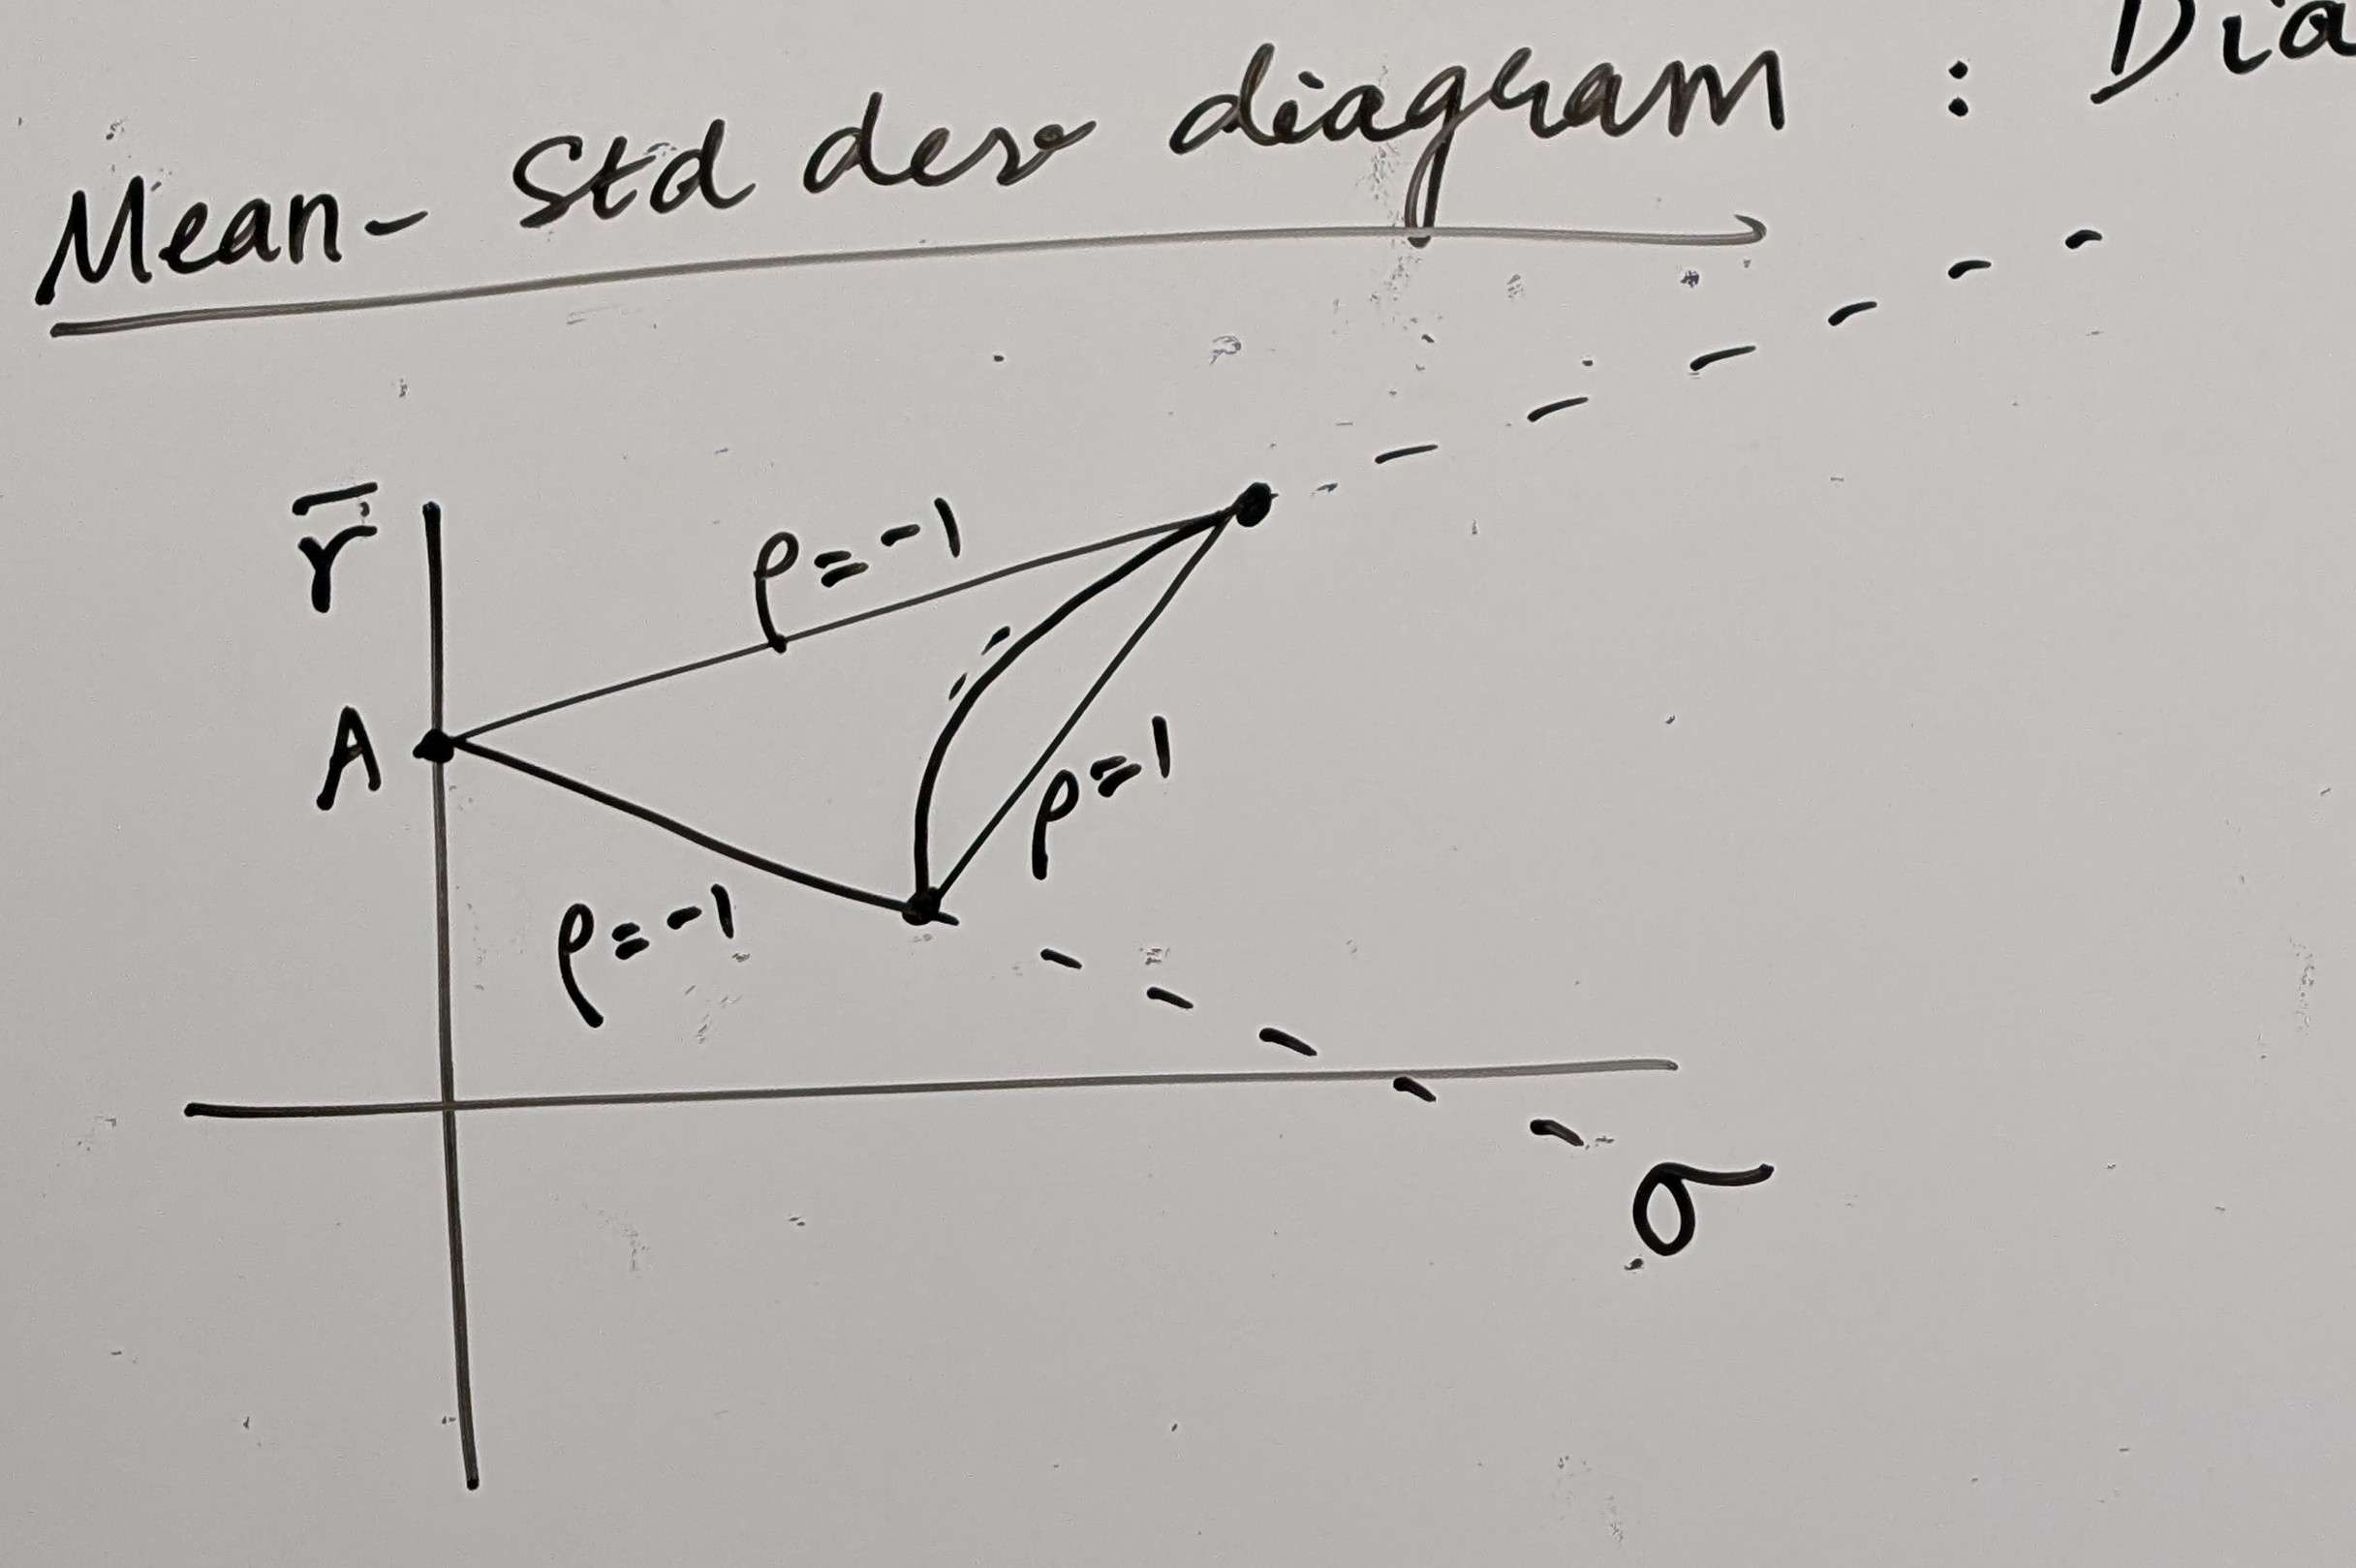
\includegraphics[width=\textwidth]{PXL_20250423_212710315.jpg}

The curve in an $\bar{r}$-$\sigma$ diagram defined by a nonnegative mixture of two assets lies within the triangular region defined by two assets and a point on the verticle axis with height
\[A=\frac{\bar{r}_1\sigma_2+\bar{r}_2\sigma_1}{\sigma_1+\sigma_2}.\] Since $w_1+w_2=1,$ let $w_1=\alpha,w_2=1-\alpha.$ Then
\[\mathrm{E}[r(\alpha)]=(1-\alpha)\bar{r}_1+\alpha\bar{r}_2\]
and
\[\sigma(\alpha)=\sqrt{(1-\alpha)^2\sigma_1^2+2\alpha(1-\alpha)\Sigma_{1,2}+\alpha^2\sigma^2}=\sqrt{(1-\alpha)^2\sigma_1^2+2\alpha(1-\alpha)\sigma_1\sigma_2\rho +\alpha^2\sigma^2}.\]
If $\rho=1,$ then $\sigma=(1-\alpha)\sigma_1+\alpha\sigma_2.$ If $\rho=-1,$ then $\sigma(\alpha)=|(1-\alpha)\sigma_1-\alpha\sigma_2|.$
We can then solve for $A$ to get
\[\frac{\bar{r}_1\sigma_2+\bar{r}_2\sigma_1}{\sigma_1+\sigma_2}.\]
We can extend this to $n$ assets. We can plot the $n$ points in our plane and find all the combinations of the assets, still assuming $\sum_i w_i=1.$ The set of all points that correspond to these portfolios is called a feasible set.

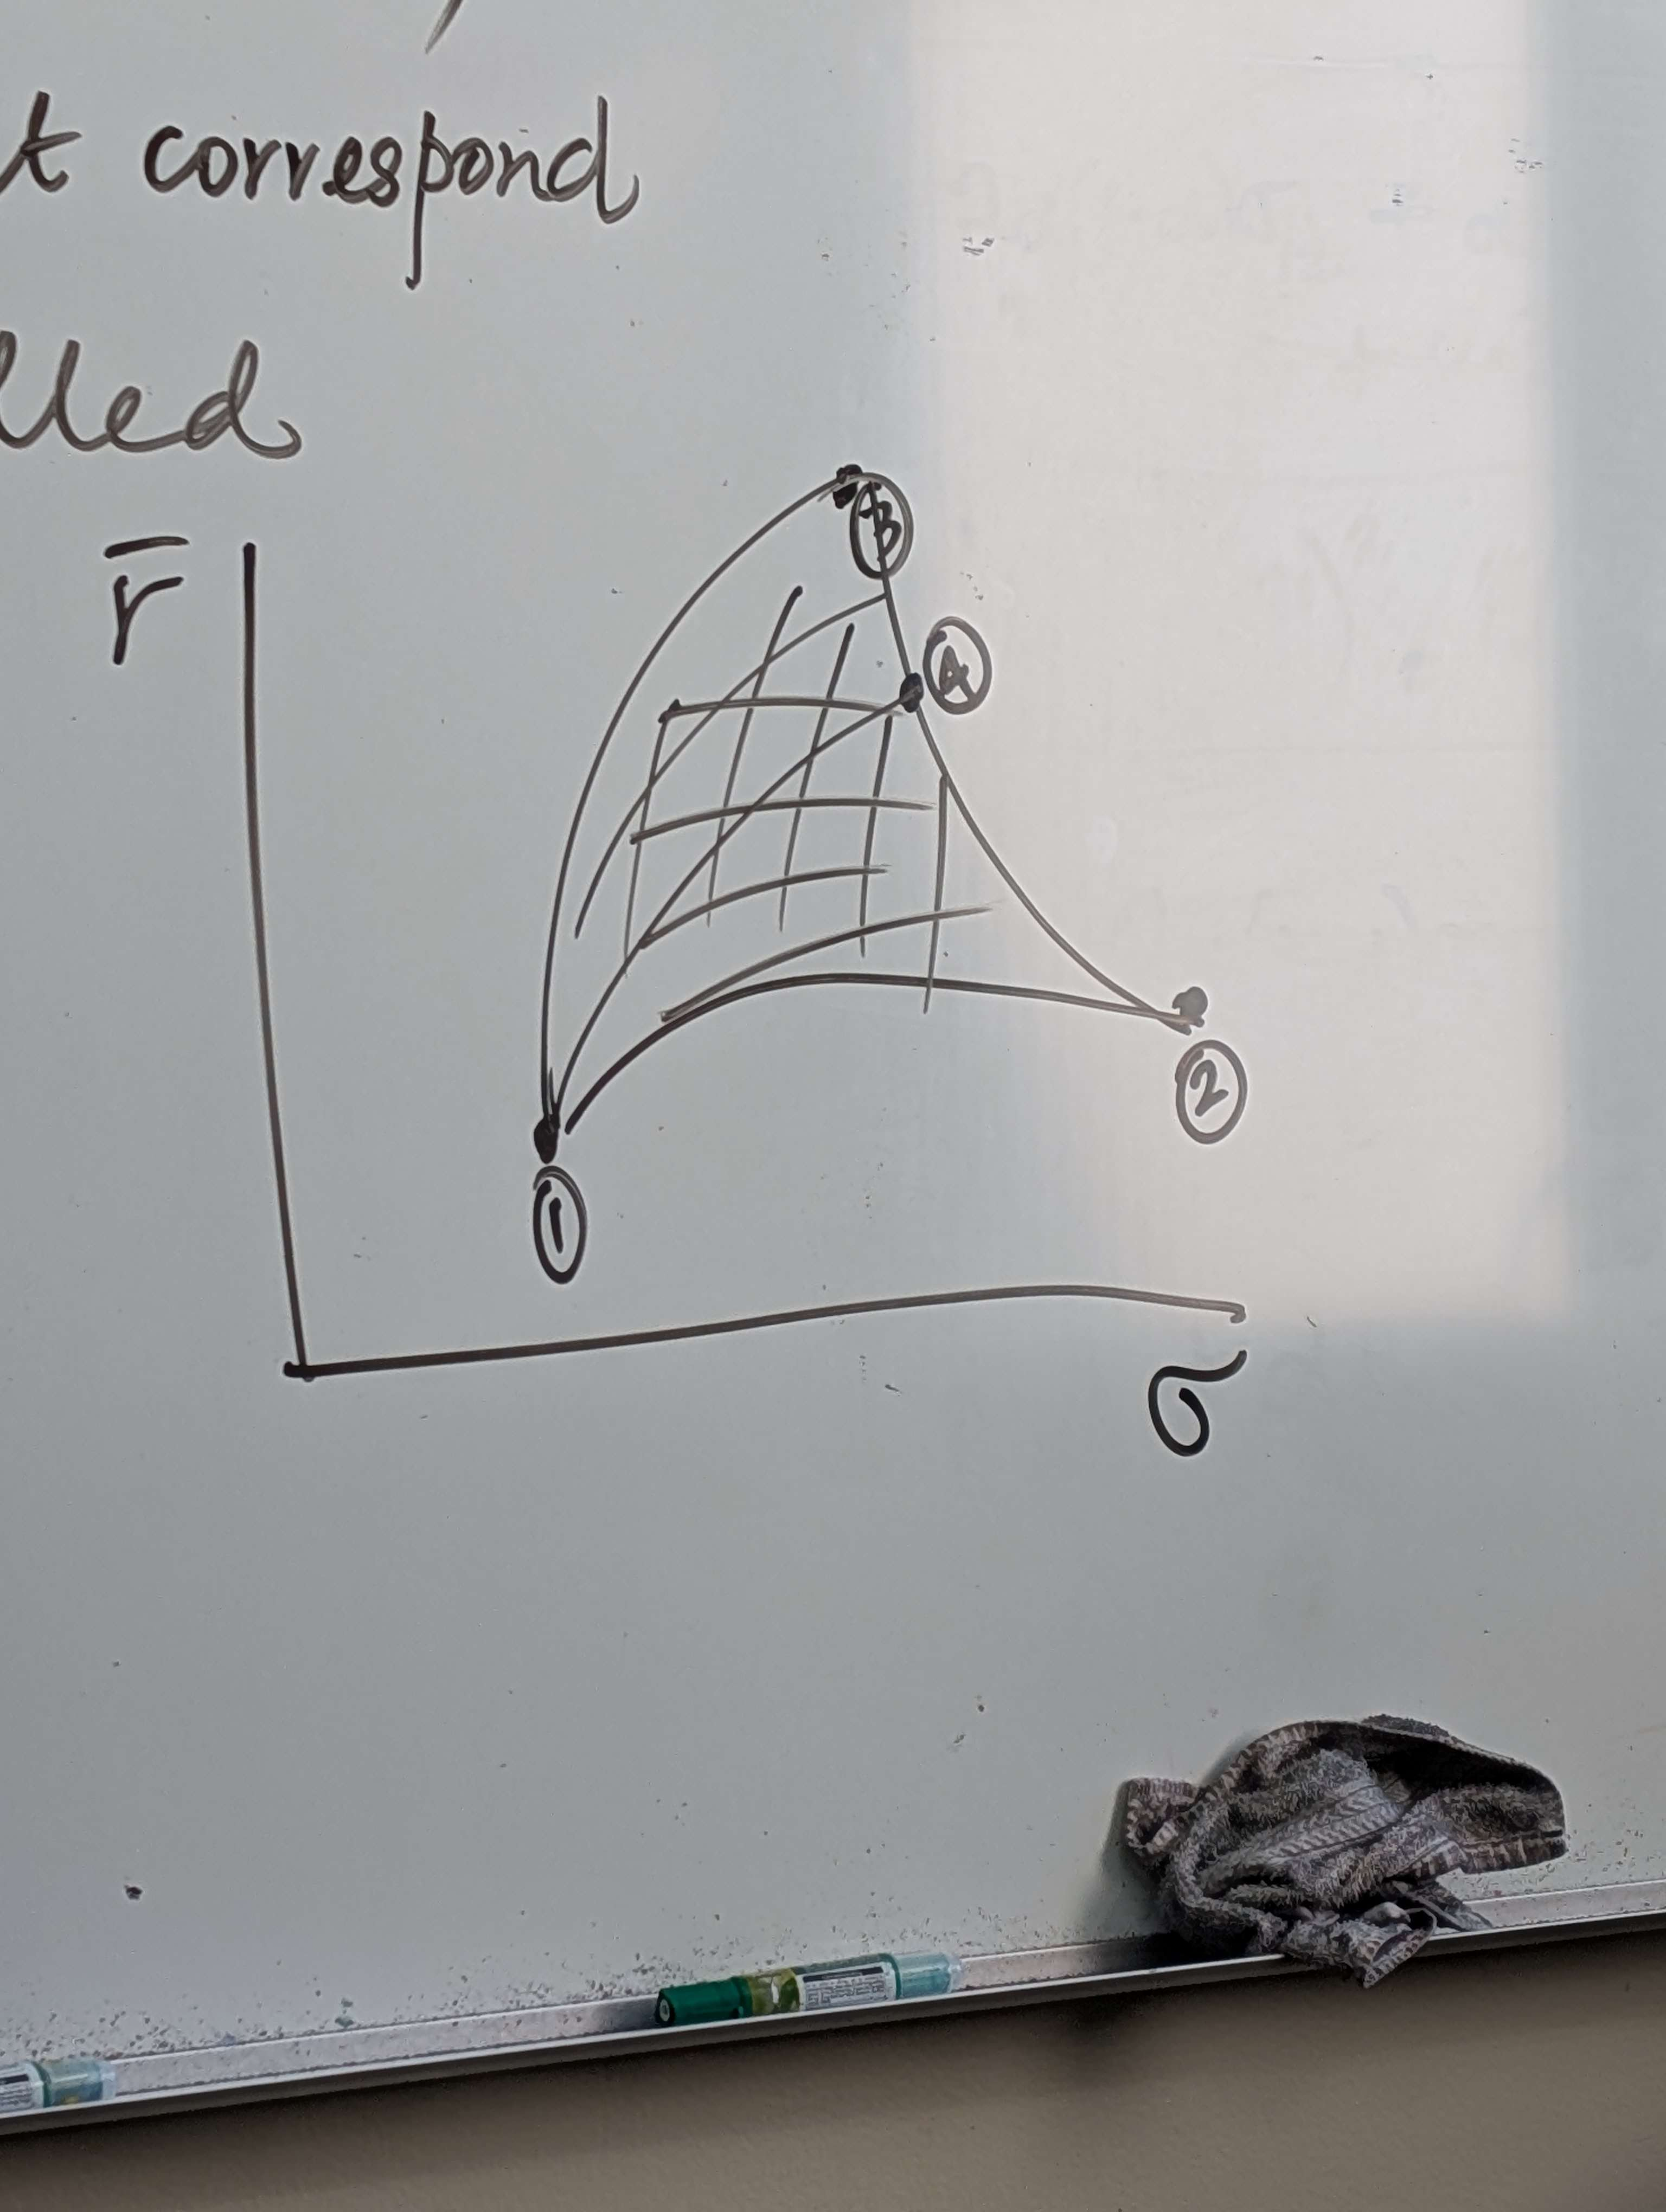
\includegraphics[width=\textwidth]{PXL_20250423_215039661.jpg}

This set is left-convex, so the segment between two points in the feasible region will not cross the left boundary of the set. Shorting lets you extend further to the right.

For a certain $\sigma,$ we want the highest $\bar{r},$ and for a fixed $\bar{r},$ we want the lowest $\sigma.$ We define the minimum variance set to be the leftmost boundary of the feasible set (between 1 and 3 on the diagram).

\subsection{Feasible Region cont. (2025.04.25)}
For a fixed $\sigma$, we would want to maximize $\bar r$, while for a fixed $\bar r$ we minimize $\sigma$ to minimize risk. Thus, there is a frontier (\url{https://en.wikipedia.org/wiki/Pareto_front}) that is basically the only part of the feasible region that matters. This left boundary of our $\bar r$-$\sigma$ graph is called the \emph{minimum variance set}. The \emph{efficient frontier} is a subset of the minimum variance set, and it is the upper portion where $\bar r$ is above some threshold.

The Markowitz Model seeks to calculate the points on the efficient frontier. We have $n$ assets with expected returns $\bar r_1, \bar r_2, \dots, \bar r_n$ and covariances $\Sigma_{i,j}$. We invest with (possibly negative) weights $w_i$ where $\bar r = \sum w_i \bar r_i$. We fix the overall mean $\bar r$ and find a feasible portfolio of minimum variance with this mean return. The problem is thus \[\min_{w_i} \frac{1}{2}\sigma^2 =\min_{w_i}\frac{1}{2} \sum w_i w_j \Sigma_{i,j}\] under the constraints \[\sum w_i \bar r_i = \bar r \qquad \sum w_i = 1.\] (the $\frac{1}{2}$ is just for convenience).

\paragraph{Example with 2 assets} 
\[\mathcal{L} = \frac{1}{2} \left(w_1^2 \sigma_1^2 + w_2^2 \sigma_2^2+2w_1w_2\Sigma_{1,2}\right) - \lambda \left(w_1 \bar r_1 + w_2 \bar r_2 - \bar r\right) - \mu \left( w_1 + w_2 - 1\right)\]
\[ \frac{\partial \mathcal{L}}{\partial w_1} = w_1 \sigma_1^2 + w_2 \Sigma_{1,2}-\lambda \bar r_1 - \mu = 0.\]

We have the same thing for $w_2$ by symmetry, and we can just solve this system using linear algebra.

\paragraph{Example: 3 uncorrelated assets}
We have 3 uncorrelated assets with variance 1. $\bar r_1 = 1, \bar r_2 = 2, \bar r_3 = 3$. Where is the minimum return and lowest risk?
\[\sigma^2=\sum_{i,j} w_i w_j \Sigma_{1,2} = \sum_i w_i^2 \qquad (\Sigma_{i,j} = \delta_i^j)\]
\[\mathcal{L} = \frac{1}{2}\sum w_i^2  - \lambda\left(\sum w_i \bar r_i - \bar r\right) - \mu \left(\sum w_i - 1\right)\]
\[\frac{\partial \mathcal{L}}{\partial w_i} = w_i - \lambda \bar r_i - \mu = 0.\]

Ok trust me the solution turns out to be $w_i = \frac{1}{3}$, $\bar r = 2$, $\sigma = \frac{1}{\sqrt 3}$.

\paragraph{Linear Combination}
Suppose I know that there are 2 known solutions on the efficient front: some $\vec w_1$, $\lambda_1$, $\mu_1$ along with $\vec w_2$, $\lambda_2$, $\mu_2$ for a different $\bar r_2$. If I form a linear combination of $\bar r = \alpha \bar r_1 + (1-\alpha) \bar r_2$, then $\alpha \vec w_1 + (1-\alpha)\vec w_2$ is a point on the efficient front. The weights are thus linear, but the $\sigma$ need not be. This motivates us to find the two simplest portfolios we can have to span the space of the efficient front.

\subsubsection{Two Fund Theorem}
Two efficient funds can be established such that any efficient portfolio (in terms of mean and variance) can be duplicated as a combination of these two. As an investor, you only need to invest in combinations of these two funds to do anything. The simplest scenarios are $\lambda = 0, \mu = 1$ and $\mu = 0, \lambda = 1$.

\section{Presentations}
\subsection{Entropy of Chinese (2025.04.25)}
Marcus, Jonny, and possibly Daniel.

\subsubsection{Gendered Language (Jonny)} Why is it effective when it seems arbitrary? Reducing entropy of the next word: Spanish `la' reduces the possibilities of what comes next more than English `the'. German is an extreme example of a gendered language, gender also carries semantic meaning:
\begin{enumerate}
    \item masc: der band $\to$ volume
    \item neu: das band $\to$ ribbon
    \item fem: die band $\to$ musical band
    \item any plural: die
\end{enumerate}

Why not gendered, or what does English have in place of gender? Adjectives, other constructions. Study: speakers of gendered languages scan for words that agree in gender upon encountering a gendered word. Efficient for attending to words that go together?

\paragraph{TTR (Type Token Ratio)} as a measure of complexity. \[\frac{\text{\# of unique words}}{\text{\# of total words}}\]
This is some constant for english: $\frac{1}{2.12}k$ vs. $\frac{1}{4.93}k$ for German. How does English convey meaning differently from German? There are two main theories: 1) that English does not have a diverse vocabulary but specificity comes from adjectives, or 2) that English is diverse and adjectives merely facilitate.

\[\text{dog} \to \text{retriever} \to \text{daschund}\] In the first theory, dog should be modified the most while daschund the least to achieve the desired specificity. The opposite is predicted by the second theory. 

We graph the frequency of an adjective vs. the entropy. Supports theory 1? Whereas German conveys meaning with articles/gender, English does it with adjectives. Adjectives reduce the entropy of the next word in English while articles do the same in German. Adjectives come before the noun in English, whereas in other languages they come after.

Gender's purposes: Ease of learning, efficiency in communication. Tradeoffs in what's important.

Redundancy of adjectives: Why say `cute little puppy' or `nice cold beer'? Adding redundancy reduces entropy of next word and adds resistance to errors.

\subsubsection{Chinese (Marcus)}
Idiosyncratic classifiers are the exceptions to the general rules for things like `yi ge.' High entropy, makes the language harder to learn.

Conditional entropy $H(C|X)$ should be near 0 as the classifier should be determined by the word, and mutual information $I(C;X)$ should be high for idiosyncratic classifiers. Remember that
\[I(C;X)=H(C) - H(C|X).\] The X can be nouns or other things like semantic classes. We can calculate these quantities:
$H(C) = 5.61$, $H(C|N)=0.66$, $I(C;N) = 4.95$ where $N$ is a noun. $H(C|S) = 1.47$ where $S$ is a semantic class.

These idiosyncrasies seem to be relics from how the language evolved, and info theory can be used to quantify idiosyncrasies. 

\subsection{Generalizations of Entropy (2025.04.29)}
Jacqueline and Ainslie

\paragraph{Jacqueline}
Renyi Entropy is a generalization of Shannon Entropy $H(X)=-\sum p_i \log p_i$. Shannon occurs as a special case of Renyi with $\alpha = 1$.

\[H_\alpha = \frac{1}{1-\alpha} \log\left( \sum  p_i^\alpha\right)\qquad0\le\alpha<\infty\]
There are singularities at $\alpha = 1,0,\infty$ and they are some interesting cases. To show that Shannon occurs in the limit as $\alpha = 1$, we use L'Hoptial's rule
\begin{align}
   \lim_{\alpha\to1} \frac{\log\left(\sum p_i^\alpha\right)}{1-\alpha} = \lim_{\alpha\to1} \frac{\left(\sum p_i^\alpha\right)^{-1} \dots}{-1}
\end{align}

Properties of Renyi entropy:
\begin{enumerate}
    \item Regardless of $\alpha$, $H_\alpha(X)$ is the same for uniform $X$. In this case, all $p_i = \frac{1}{n}$ and \[H_\alpha(X) = \frac{1}{1-\alpha} \log\left(n n^{-\alpha}\right) = \frac{1-\alpha}{1-\alpha}\log n.\]
    \item Renyi entropy is convex. The binary Renyi entropy function looks like this \autoref{renyi}. 
\begin{figure}
    \centering
    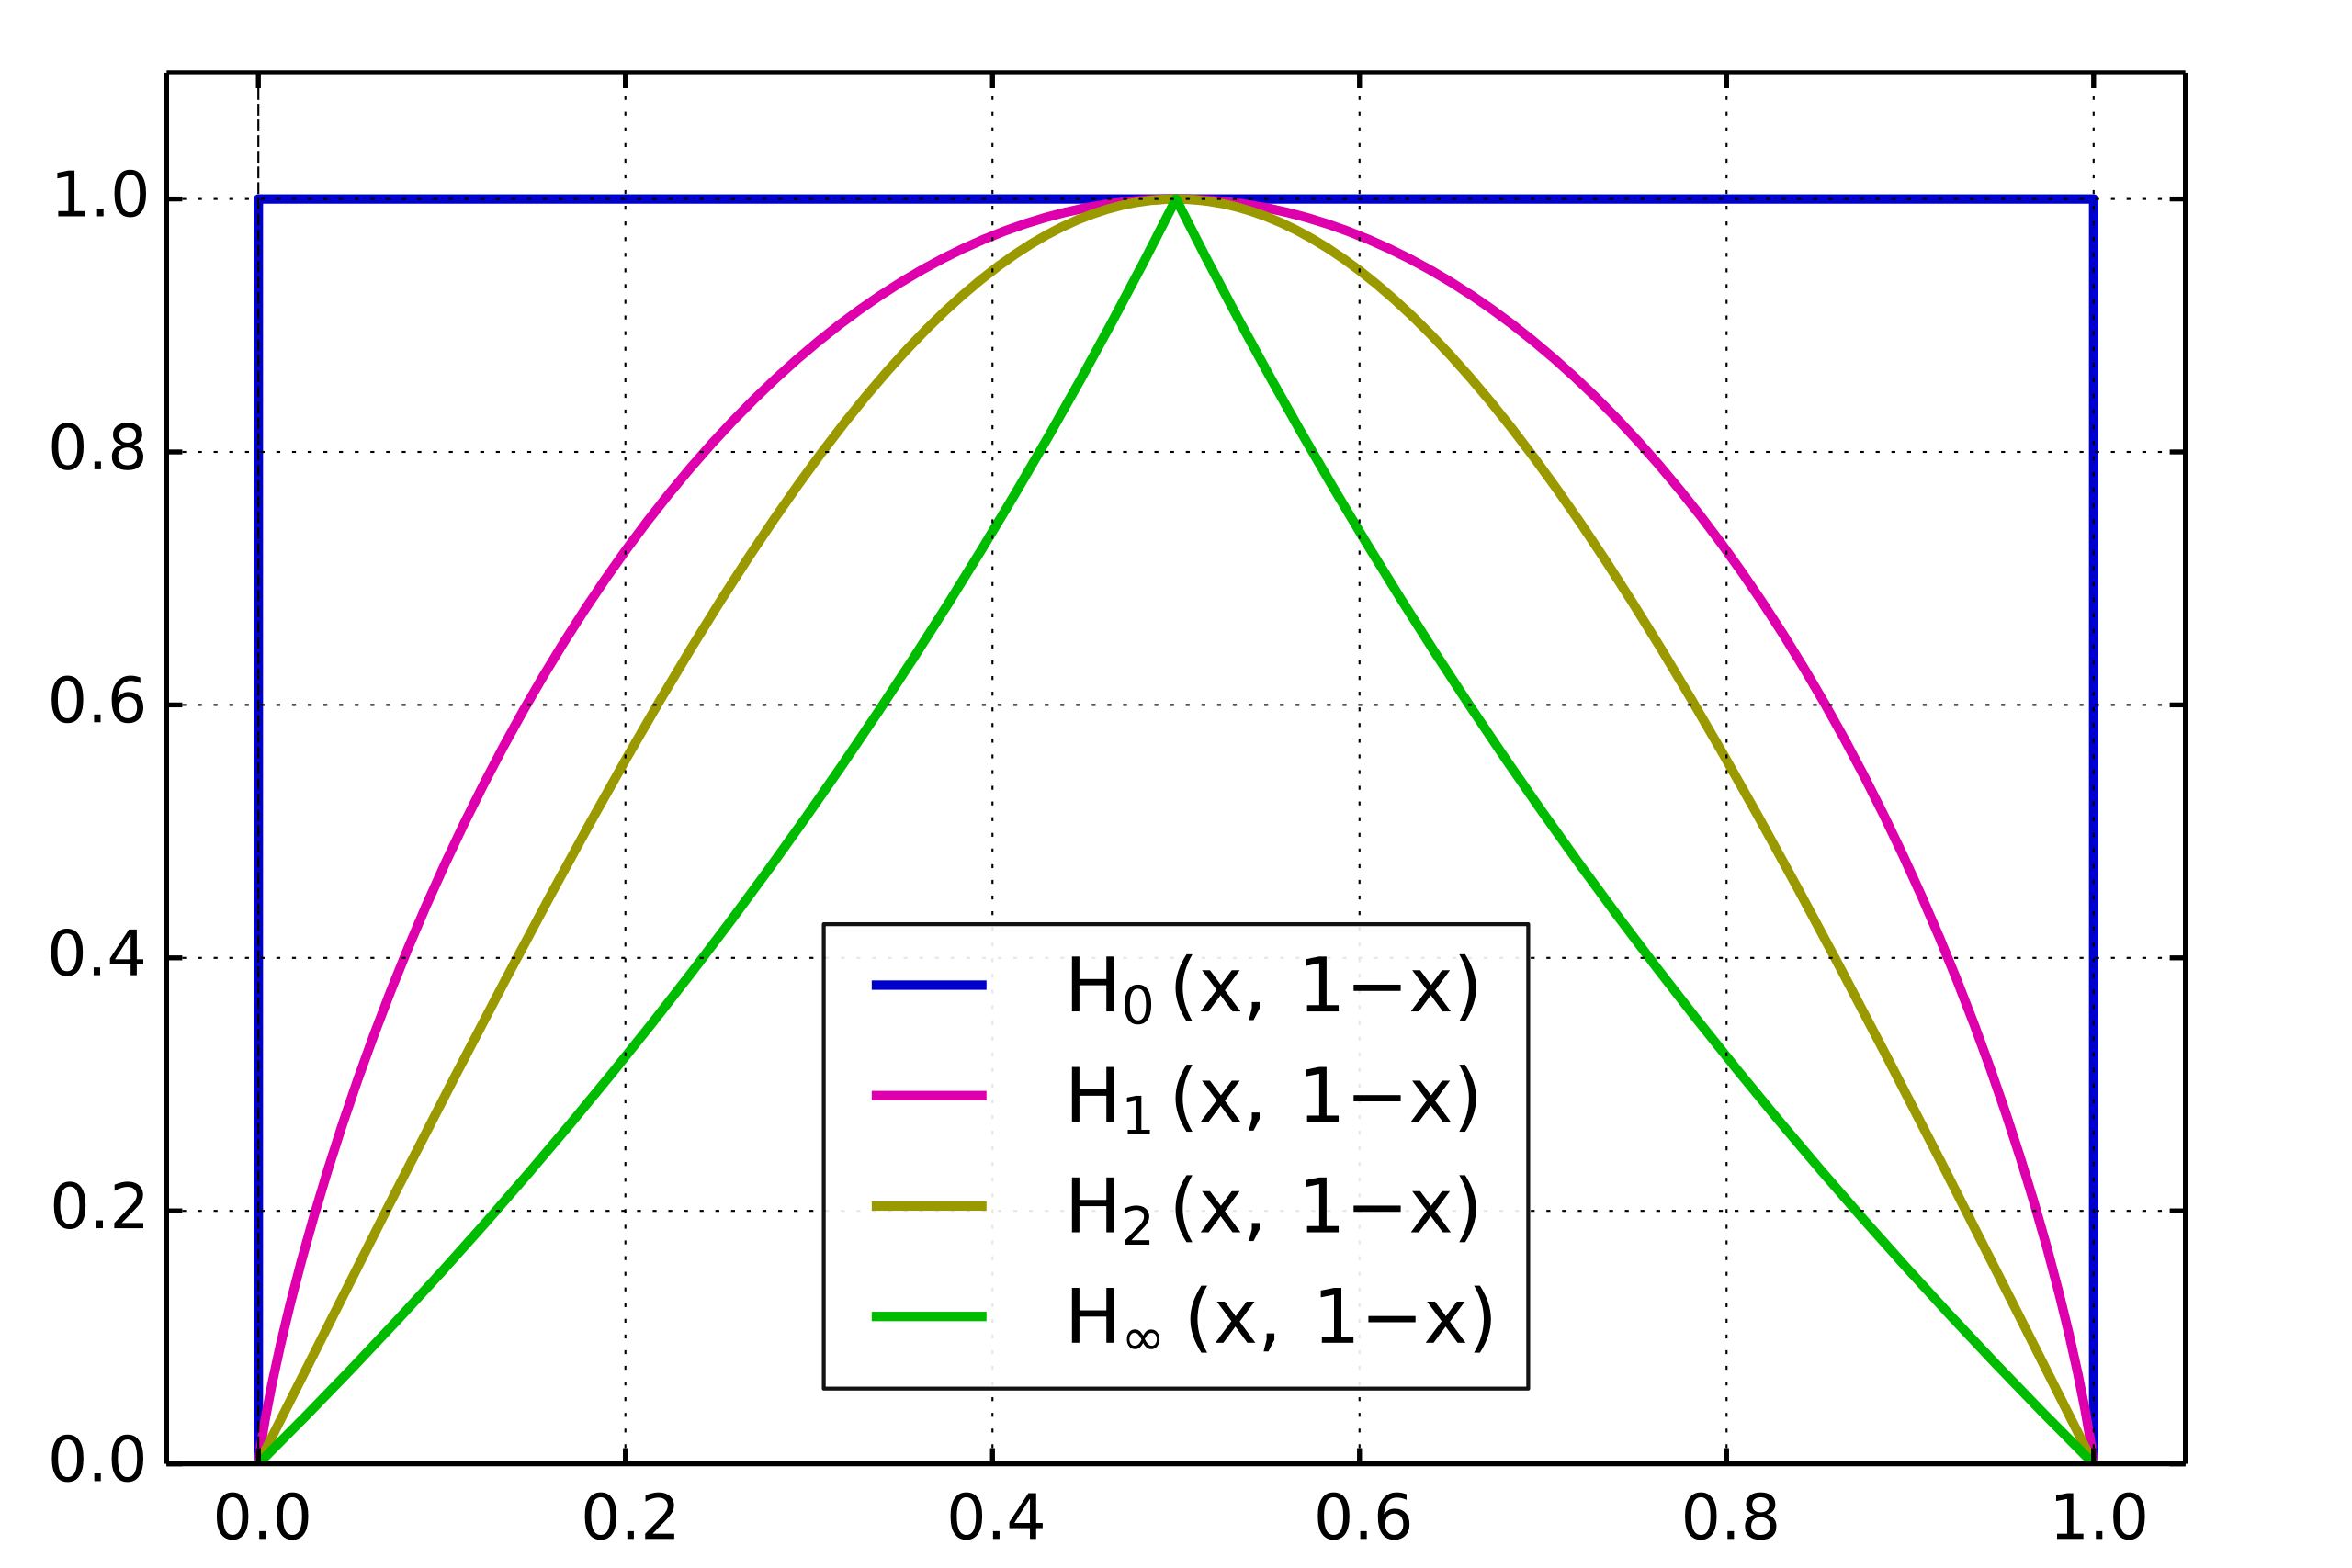
\includegraphics[width=0.5\linewidth]{image2.png}
    \caption{Binary Renyi entropy is convex.}
    \label{renyi}
\end{figure}
    Thus, for a fixed random variable, the Renyi entropy is decreasing with respect to $\alpha$.

    \item As $\alpha$ approaches 0, it weights probabilities more equally. This is Hartley entropy: \[H_0(X)=\log n.\]

    \item For $\alpha=\infty$, we can ignore all $p_i$ except for the biggest $p_i$. The Renyi entropy is thus approximately
    \[H_\infty(X)=\frac{\alpha}{1-\alpha} \log(\max p_i)=-\log(\max p_i).\]
    This is min-entropy, where we do not care about any outcomes other than the most probable one.
\end{enumerate}


\paragraph{Ainslie: Applications to Ecological diversity}

An important metric is species richness. Given $n$ species with $p_i$ relative abundance each, $\sum p_i$ is the species richness. The \emph{shannon index} is the entropy of $p_i$, $-\sum p_i \log p_i$. The \emph{Simpson's index} is $\sum p_i^2$, and it is a similarity index quantifying how likely two individuals are from the same species.

Hill defines a Hill number, and it is related to the Renyi entropy:
\[D = \left( \sum p_i^q\right)^\frac{1}{1-q} = 2^{H_q(\vec{p_i})}.\]
As $q\to1$, $D$ approaches shannon entropy/shannon index, and as $q\to2$, $D$ approaches the inverse of Simpson's index.

Aw and Rosenberg comes up with more metrics: For genetics, the three outcomes that matter are homozygous $AA$, $aa$, and heterozygous $Aa$. Expected homozygocity $J$ and exepcted heterozygocity $H$ can be quantified with
\[J^{(q)}(p)=\sum p_i^q\]
\[H^{(q)}(p) = 1- J^{(q)}\]
The $q$ depends on the number of alleles, humans are diploid so $q=2$.

This can connect to Renyi entropy
\[H_q = \frac{1}{1-q}\log J^{(q)}\]
\[D_q = 2^{H_q}\]

Another thing we can do is generalize Kullback-Liebler with Renyi divergence:
\[D_\alpha(P\mid\mid Q)=\frac{1}{\alpha - 1} \log \left(\sum p_i^\alpha q_i^{1-\alpha}\right).\]

We can show in the limit as $\alpha\to1$ this approaches Kullback-Liebler. I don't want to write this.

Also financial applications: the expected rate can be
\[\frac{1}{R} D_1(b\mid \mid m) + \frac{R-1}{R} D_{1/R}(b \mid \mid m).\]

\subsection{Info Theory in Linguistics (2025.04.29)}
Alex Huang and Aarush Vailaya

\paragraph{What is linguistics?} Scientific study of language. Phonetics (sound, phonemes), syntax/grammar, semantics (meaning), morphology, phonology (sound system/inventory).

Sociolinguistics, developmental linguistics, neurolinguistics, applied linguistics. 

\paragraph{Zipf's Law} In a list of measured tokens sorted in decreasing frequency, the $n$th entry has frequency of approximately $1/n$. The most common word in a language is twice as common as the next, 3x as common as 3rd, etc.

Word length and information content. The average information content is a better predictor of word length an frequency. 

Let $C$ be context (previous $n$ words in the n-gram model) and $W$ be word. The average info content is the entropy(?)
\[-\sum P(C|W) \log P(W|C).\]

Using an $n$-gram model, we can test our hypothesis. This hypothesis holds for most languages in 2, 3, and 4-gram models. Polish and Swedish are not nice though. The correlation between word length and frequency was weaker than info content and frequency.

\paragraph{Aarush: Language acquisition:} There seems to be a strong lack of negative feedback in acquiring language for babies. You never tell a baby that what they said is wrong, you only really provide a wide array of correct sentences. How do you not end up with over-general rules?

Solomonoff induction is a formalization of Occam's razor. The prior $\lambda$ is the base hypothesis, that some random program is producing the output that we see. We can reuse some Kolmogorov ideas.
\[\lambda(n) = \sum_\text{valid programs that produce $n$} 2^{-\ell(p)}\]
$\lambda(n)$ is our estimate for the probability of outputting $n$, and this is biased towards short programs due to the process of selecting a random program (start writing random bits until its a halting program). We start by saying that all random programs are valid, then getting rid of any programs that do not match what we see at each step. This is effectively computing conditional probabilities, conditioned on preceding context.

At the start, many programs would output the thing, but we throw away possibilities as we see more and more input. Solomonoff induction is that $\lambda$ will approach the behavior of the real program/probabilities $P$ as we see more and more output.
\[\sum^\infty [P(x_i|x_1,x_2,\dots)-\lambda(\dots)]^2=\text{constant}\]

Assume that babies are Turing-complete. Upon seeing an infinite number of correct sentences, they will converge on the exact program that produced those sentences.

\subsection{Neil's thing (2025.04.29)}
\paragraph{Delsarte Linear Program} We have some variables in $\vec x$, and we want to minimize $A\vec x$ under the constraints $B\vec x \ge \vec 0$.

Let us try to write the problem of optimizing codes in a linear program. We have code words and errors. To find codewords of length n that minimize error from, I want a set of codewords $C\subseteq \mathbb{Z}_2^n$ where Hamming distance $d(c_1,c_2) \ge d$ for all codewords $c_1,c_2\in C$. I want to find the largest such subset $C$.

Now we do the cube thing. For example we have $\mathbb{Z}_2^2$, we can draw a graph between all elements with edges colored according to the hamming distance between them. We can also do this by defining the set $R_i = \{(c_a,c_b):d(c_a,c_b)=i\}$.

\begin{enumerate}
    \item $R_0 = \{(c,c)\}$
    \item $R_i = \{(c_a,c_b):d(c_a,c_b)=i\}$
    \item Let $p_{i,j}^h$ be the number of codewords $z$ such that there exist $x,y$ where $d(x,y)=h$, $d(x,z)=i$, and $d(z,y)=j$. We count the number of $z$ where we can find $h$-apart codewords that are $i$ and $j$ away from $z$. For example, $p^3_{1,1}=p^2_{1,2}=0$, $p^3_{1,2}=3$.
\end{enumerate}

Matrix interpretation of the graph/sets $R_i$:
Let $A_i$ be the adjacency matrix corresponding to $R_i$ (or the edges of a certain color in our graph). For our example our matrices are nice. $A_0$ is the identity, $A_2$ is 1s on the other diagonal, and 
\[A_1 = \begin{bmatrix}
    0 & 1 & 1 & 0 \\ 1 & 0 & 0 & 1 \\ 1 & 0 & 0 & 1 \\ 0 & 1 & 1 & 0
\end{bmatrix}\]

If we multiply matrices, we have $A_jA_i = \sum_{h=0}^n p_{i,j}^h A_h$ for some reason. Because multiplication is a linear combination of the base matrices, we can build a Bose-Mesner algebra, closed under multiplication and addition. Multiplication is commutative in this algebra. The $A_i$s are a basis for this algebra, but we also have another basis $E_i$ defined such that
\[E_iE_j = \begin{cases}
    0 & i\ne j \\
    E_i & i = j
\end{cases}\]
These are the projectors.
\[E_0 = \frac{1}{4}(A_0 + A_1+A_2)\]
\[E_1 = \frac{1}{2}(A_0 - A_2)\]
\[E_2 = \frac{1}{4} (A_0 - A_1 + A_2)\]

We can also find eigenmatrices. There exists a matrix $P$ such that 
\[\begin{bmatrix}
    A_0 & A_1 & \cdots
\end{bmatrix} = \begin{bmatrix}
    E_0 & E_1 & \cdots
\end{bmatrix} P\]
and this matrix $P$ is invertible even though we are dealing with integer matrices. 

\[P = \begin{bmatrix}
    1 & 2 & 1 \\ 1 & 0 & -1 \\ 1 & -2 & 1
\end{bmatrix}\]

To find the set of codewords we solve the following linear program:
$\vec a$ is the distribution such that
\[a_i = \frac{|(C\times C) \cap R_i|}{|C|}\]
\begin{enumerate}
    \item $a_0 = 1$
    \item $a_i = 0$ for $1 \le i \le d$, where $d$ is the original restriction for the minimum distance between codewords.
    \item $a_i > 0$ for all i
    \item $\sum a_i = |C|$
    \item $\vec a P \ge 0$
\end{enumerate}

\subsection{Quantum Information (2025.05.01)}
Grant and Rohan
\paragraph{Fundamentals of Quantum Computing}
\begin{enumerate}
    \item In Quantum Mechanics, objects no longer have a single deterministic state like a classical object and are instead in a superposition.
    \item For example, uncertainty in position and uncertainty in momentum are inversely proportional (Heisenberg Uncertainty).
    \item So instead of using a point in phase space to describe an object, we use a \textbf{state vector $\ket{\psi}$,} which can be thought of as a linear combination of some basis states
    \item However, for this presentation, we will be focusing on discrete states which attain discrete values, such as the states of an electron: spin up ($\ket{\uparrow_x}$) or spin down ($\ket{\downarrow_x}$).
    \item Not only can we have states like $\ket{\uparrow_x}$ and $\ket{\downarrow_x}$ but also $\frac{1}{\sqrt{2}}\ket{\uparrow_x}+\frac{1}{\sqrt{2}}\ket{\downarrow_x},$ which might represent spin right ($\ket{\uparrow_{z}}$).
    \item By the Born Rule (see later), this particle has a $0.5$ probability of being measured spin up and a $0.5$ probability of being measured spin down.

    \item The Kronecker product $\otimes$ is used to glue two quantum states together.
    \[
    (a_1 \ket{\uparrow}+a_2\ket{\downarrow})\otimes(b_1 \ket{\uparrow}+b_2\ket{\downarrow}) =\]
    \[a_1 b_1 \ket{\uparrow}\otimes\ket{\uparrow}+a_1 b_2 \ket{\uparrow}\otimes\ket{\downarrow} + a_2 b_1 \ket \downarrow \otimes \ket \uparrow + a_2 b_2 \ket \downarrow \otimes \ket \downarrow \]
    This is also how we describe entangled pairs of particles: $\frac{1}{\sqrt 2}\ket{\uparrow}\otimes\ket \downarrow + \frac{1}{\sqrt 2} \ket \downarrow \otimes \ket \uparrow$.
    \item For convenience, we will omit the Kronecker product symbol when writing it out, e.g.
    \[\ket{0}\otimes\ket{0}\to\ket{00}.\] But, do not forget that the Kronecker product is still there.
\end{enumerate}

\paragraph{How Quantum is Different}
\begin{enumerate}
    \item Say you have a mixture of quantum states:
    
    50\% spin right $\ket{\uparrow_x}$, 50\% spin up $\ket{\uparrow_y}$.
    \item Classically, this is 1 bit of information.
    \item However, you cannot make a measurement without skewing the distribution away from 50-50! The least you can disturb it is with a 45-degree axis, yielding only $H(\cos^2\frac{\pi}{8})\approx0.6$ qubits. 
    % (its $\frac{\pi}{8}$ because quaternions double cover $SO(3)$).

    \item Because of entanglement, we can also do funny stuff like send 2 classical bits in 1 qubit given a shared entangled bit (superdense coding).
\end{enumerate}

\paragraph{The Born Rule and Dirac-von Neumann Axioms}
\begin{enumerate}
\item $\ket{\psi} = c_1 \ket{a} + c_2 \ket{b} + \dots,\qquad c_1,c_2,\dots\in\mathbb{C}$
\item $P(\psi\text{ is in state }a)= \left\lvert\braket{a|\psi}\right\rvert^2$
\item $\braket{\psi|\psi} = 1, \quad \braket{a|b} = 0$. \qquad $\bra{\psi} = c_1^\ast \bra{a} + c_2^\ast \bra{b} + \dots$

\item Any observable can be represented as an operator (matrix) $\hat A$. The expected value of $\hat A$ is denoted
$\braket{\hat A} = \bra{\psi}\hat A\ket{\psi}$.

\begin{enumerate}
    \item Let $\ket{A_i}$ be a set of eigenvectors of $\hat A$. Assuming that the eigenvectors are non-degenerate, we can get an \textbf{orthonormal} basis that spans the space of quantum states (spectral theorem).
    
    \item If we express $\ket{\psi}$ in this basis and interpret the eigenvalues $a_i$ as the values for the observable, $\braket{\psi | \hat A |\psi}$ reduces to the usual formula for expected value! 
\end{enumerate}
\end{enumerate}

        \begin{align*}
        &\hat A = \sum_i a_i \ket{A_i}\bra{A_i}\\
        &\ket{\psi} = \sum_i c_i \ket{A_i} \\
        &\hat A \ket{\psi} = \sum_i a_i c_i \ket{A_i} &&\quad \hat A \ket{A_i} = a_i\ket{A_i}
    \end{align*}
        \[
        \braket{\psi|\hat A| \psi} = \sum_i a_i c_i^\ast c_i = \sum_i a_i P_\psi(\ket{A_i})=\langle\hat A\rangle 
        \]


% \url{https://en.wikipedia.org/wiki/Dirac%E2%80%93von_Neumann_axioms}

\paragraph{Mixture States and the Density Matrix}
    \begin{enumerate}
        \item The density matrix is a more generalized way to write a wavefunction that allows you to deal with mixture states.

        \item $\rho = \ket{\psi}\bra{\psi}$, so the probability of measuring state $a$ is $\bra{a}\rho\ket{a}$. $\rho$ is an observable representing `how likely is $\psi$?' and $\braket{\hat A} = \mathrm{tr}(\hat A \rho)$.
        \begin{align*}\mathrm{tr}(\hat A \rho) &= \mathrm{tr}\left[\left(\sum_i a_i \ket{A_i} \bra{A_i}\right)\left(\sum_{j,k} c_j c_k^\ast \ket{A_j}\bra{A_k}\right)\right] \\
        &= \mathrm{tr}\left[\sum_{i,k}a_i c_i c_k^\ast \ket{A_i}\bra{A_k}\right]=\sum_ia_i|c_i|^2\ket{A_i}\bra{A_i}=\langle\hat A\rangle.
        \end{align*}

        \item If we want to represent a \emph{mixture state} instead, that is a distribution of possible states, we can just do $\rho = \sum_i p_i \ket{\psi_i}\bra{\psi_i}$. We can't use wavefunctions because those can only handle superpositions, not mixtures! Think about the expected value formulae.
    \end{enumerate}

    % https://ocw.mit.edu/courses/5-74-introductory-quantum-mechanics-ii-spring-2009/a1a6a947e655c9e9af9a9e5aa3b99cc9_MIT5_74s09_lec12.pdf

\paragraph{Von Neumann Entropy}
    
    \begin{enumerate}
        \item \[S = -\mathrm{tr}(\rho \ln \rho)\]
        \item A \textbf{projector} is an operator such that $\Pi^2 = \Pi$. For example, $\Pi= \ket{x}\bra{x}$. If we sum the projectors for each basis vector in an orthonormal basis, we get the identity. Projectors are important because they represent the process of measuring and collapsing a possibly mixed quantum state.
        \item We can show that \[S = \min_{\{\Pi_{1,2,\dots}\}} \left[ -\sum_i\mathrm{tr} (\Pi_i\rho) \ln(  \mathrm{tr}\,(\Pi_i \rho)) \right]\]
        \begin{itemize}
            \item where the minimum is taken over all sets of projectors such that $\sum_i \Pi_i = I$ and for each projector $\mathrm{tr}(\Pi_i)\le1$.
        \end{itemize} 
        \item In other words, $S$ is the absolute minimum amount of uncertainty under the most efficient measurement we can make, which happens to be in the orthonormal eigenbasis.
    \end{enumerate}
    % https://arxiv.org/pdf/1106.1445


Since $\rho$ is a hermitian matrix (i.e. $\rho^\dagger=\rho$),
    \[\rho=\sum_i p_i\ket{\psi_i}\bra{\psi_i}=\sum_i\eta_j\ket{j}\bra{j},\]
where $\ket{j}$ are orthonormal eigenvectors with eigenvalues $\eta_j.$ Furthermore, by Born's rule, the eigenbasis measurement is optimal for distinguishing states. Since the probability of measuring $\ket{j}$ is $\eta_j,$ it's natural to set 
$S=-\sum_j\eta_j\log\eta_j.$ Also, note that, for some unitary $U$ and some real diagonal matrix $D$ and using the matrix logarithm,
\begin{align*}-\mathrm{tr}(\rho\log\rho)&=-\mathrm{tr}(UDU^\dagger U\log D U^\dagger)\\&=-\mathrm{tr}(UD\log D U^\dagger)\\&=-\mathrm{tr}(D\log D)\\&=-\sum_j \eta_j\log \eta_j=S.\end{align*}

\paragraph{Schumacher Compression}
Recall Shannon's source coding theorem:
\begin{theorem} (Source Coding Theorem)
If we send $n$ symbols drawn i.i.d. from some R.V. $X$ with entropy $H(X),$ then we can compress our codewords so that we only need to send $nH(X)$ bits, which is lossless as $n\to \infty.$
\end{theorem}
We used Huffman coding to actually implement such a compression, which achieves this rate for large $n.$ We have a similar theorem from Benjamin Schumacher:
\begin{theorem} (Schumacher Compression Theorem)
    Given $n$ qubits drawn from some source $\rho$ denoted as $\rho^{\otimes n},$ with von Neumann entropy $S(\rho),$ then we can compress the source down to $nS(\rho)$ qubits, which is lossless as $n\to\infty.$
\end{theorem}

\paragraph{An Example I}
Let's say that we want to send three qubits drawn from the distribution with $P(\psi=\ket{\uparrow_z})=P(\psi=\ket{\uparrow_x})=0.5,$ where
\[\ket{\uparrow_z}=\ket{0},\ket{\uparrow_x}=\frac{1}{\sqrt{2}}\ket{0}+\frac{1}{\sqrt{2}}\ket{1}\] in the basis $\ket{0},\ket{1}.$ We can calculate the density matrix of $\rho$ to be
\begin{align*}\rho=\begin{bmatrix}
    \frac34&\frac14\\\frac14&\frac14
\end{bmatrix}=&\lambda_{0'}\ket{0'}\bra{0'}+\lambda_{1'}\ket{1'}\bra{1'}\\=&\cos^2\frac{\pi}{8}\begin{bmatrix}
    \cos\frac\pi 8\\\sin\frac\pi 8
\end{bmatrix}\begin{bmatrix}
    \cos\frac\pi 8&\sin\frac\pi 8
\end{bmatrix}\\&+\sin^2\frac{\pi}{8}\begin{bmatrix}
    \sin\frac\pi 8\\-\cos\frac\pi 8
\end{bmatrix}\begin{bmatrix}
    \sin\frac\pi 8&-\cos\frac\pi 8
\end{bmatrix}.\end{align*}
We see that $S=H_2(\cos^2\frac\pi 8)\approx 0.601,$ and $3S<2$, so we can compress our 3 qubits into 2 qubits without losing too much information.

\paragraph{An Example II}
The probability measuring $\ket{0'}$ is $\cos^2\frac\pi 8\approx0.854,$ and the probability of measuring $\ket{1'}$ is $\sin^2\frac\pi 8\approx0.146,$ so if we measure our three qubits in the $\ket{0'},\ket{1'}$ basis, we expect for them mostly to be $\ket{0'}.$ Specifically, the probability that our message is in the set spanned by $\{\ket{0'0'0'},\ket{1'0'0'},\ket{0'1'0'},\ket{0'0'1'}\}$ is $\cos^6\frac\pi 8+3\sin^2\frac\pi 8\cos^4\frac\pi 8\approx0.942.$ 

This smaller set can be rotated to $\{\ket{000},\ket{010},\ket{100},\ket{110}\},$ and we can measure the third qubit to collapse (project) our state onto a smaller subspace. after discarding the third qubit, we have compressed our three qubits into two. The person receiving the two qubits can append $\ket{0}$ and apply the inverse of the encoding rotation to obtain their own density matrix $\rho'.$ We can calculate the \textbf{average fidelity} between $\rho'$ and $\rho$ to be around 0.923, which means that there is a 92.3\% chance that $\rho'$ and $\rho$ would be measured identically, so this is a pretty good compression.

\paragraph{The General Process}


\begin{enumerate}
    \item But wait! 92.3\% is not good enough. We want lossless, not lossy!
    \item Turns out that as $n\to\infty$ fidelity approaches 1. In general, Schumacher compression involves projecting $\rho$ into a ``typical subspace,'' the subspace spanned by the most likely eigenvectors.
\end{enumerate}

\paragraph{Typical Subspaces}
\begin{enumerate}
    \item The law of large numbers dictates that as $n\to\infty$ and for i.i.d. $X_i,$
    \begin{align*}-\log p(X^n)= -\log\prod p(X_i)&\to H(X_1,X_2,\dots,X_n) \\&= n H(X),\end{align*} where $X^n$ is a string of $n$ i.i.d. random variables $X_i.$ This is the \textbf{asymptotic equipartion property.}
    
    \item A typical subspace for some arbitrary $\delta$ is the space spanned by
    \[T_\delta =\left\{\ket{x^n}:\left|-\frac{1}{n}\log p_{X^n}(x^n)-H(X)\right|<\delta\right\}\] where $H(X)=-\sum_{x}p_X(x)\log p_X(x)=S$ and $p_X$ is our eigenvalue decomposition for $\rho=\sum_{x}p_X(x)\ket{x}\bra{x}.$ % note that we have both P_{X^N} and P_X!

    \item The probability that our sequence $\rho^{\otimes n}$ lies in this subspace is $\mathrm{tr}(\Pi\rho^{\otimes n})$, where $\Pi$ is the projector $\sum_{x^n\in T_\delta} \ket{x^n}\bra{x^n}$. 
    
    \item In the limit of infinitely long sequences, all sequences lie in the typical subspace:
    \[\lim_{n\to\infty}\mathrm{tr}(\Pi \rho^{\otimes n})=1\]. 
    
    \item However, the dimension of the subspace is bounded by $2^{n(S\pm\delta)}$. This is often significantly smaller than our full space, which is of size $2^n.$ In short, the subspace is small but the probability that $\rho^{\otimes n}$ lies in it approaches 1 asymptotically.
    \end{enumerate}

\paragraph{So What?}
    \begin{enumerate}
        \item Quantum Computing can be a very very powerful tool in certain scenarios, e.g. Grover's Algorithm, Shor's Algorithm, HHL Algorithm, allowing us to solve some very specific problems faster than any classical computer could.
        \item But, if we want to send qubits across distances, like from the output of these algorithms, it would probably be very expensive because we don't want to disturb our very delicate and complicated superposition state.
        \item So, Schumacher compression provides a scheme that allows us to (for large $n$) transmit our qubits at a better rate without loss, which will save a lot of money.
        \item We didn't mention this, but there are also error correction codes for qubits, which involves a ``syndrome'' measurement to check if the qubit is in the correct subspace. There are also theorems relating to channel theory and quantum information, but they are pretty complicated.
\end{enumerate}

\subsection{Kalman Filters (2025.05.01)}
Atharv and Aggs

Say we want to estimate the position of a car $X$, but we only have a GPS chip that gives $X+W$ where $W\sim N(0,\sigma^2)$ is some random noise. The best estimator should be the mean of all measurements, but how do we know that? An estimator is some function of all our measurements $\hat X(Z_1,Z_2,\dots,Z_n)$. A linear estimator is the best for our distributrion, so we can do $\hat X = w_1Z_1+w_2Z_2,\dots w_n Z_n.$ An unbiased estimator has the property $E[\hat X (\vec z)] = X$. To find a good estimator, let's do recursion on the base case of $\hat X_1 = Z_1$. We want an expression for $\hat X_k$ given $\hat X_{k-1}$ and $Z_k$. 
\begin{align*}
    \hat X_k &= a \hat X_{k-1} + b Z_k \\
    E[\hat X_k] &= a X + bX\qquad\therefore a+b=1
\end{align*}
The best estimator should give the most information about the variable, i.e. maximize \[I(X;Z_k|Z_{1,2,\dots,k-1})=H(X|Z_{\dots,k-1})-H(X|Z_{\dots,k})\]
Because our things are gaussian, we can expand it. To maximize mutual information, we want to minimize the variance of our variables:
\begin{align*}
    H(\hat X_{k-1}) - H(\hat X_k)=\frac{1}{2} \log \left(\frac{\sigma_{k-1}^2}{\sigma_k^2}\right).
\end{align*}

We just minimize $\mathrm{Var}[\hat X_k] = (1-t)^2 \mathrm{Var}[\hat X_{k-1}]+t^2 \sigma^2$ by setting $\frac{\partial}{\partial t}= 0$ and find that the gain \[t_k=\frac{\sigma_{k-1}^2}{\sigma^2+\sigma_{k-1}^2}\]

Update our estimate based on gain $t$ and innovation (direction to step to go from current estimate to the new data):
\[
\hat X_k = \hat X_{k-1} + t(Z_k - \hat X_{k-1})
\]

\paragraph{Matrix time} Now we upgrade everything to matrices
\[
X_k = F_k X_{k-1}+B_k U_k + W_k
\]
$W_k$ is process noise $\sim N(0,Q_k)$ where $Q_k$ is a covariance matrix. 
$U_k$ is input to the system (steering, etc) and $B_k$ transforms it into the state basis.

We measure
\[Z_k = H_k X_k+V_k\]
where $H_k$ is a matrix that transforms state to measurement, and $V_k$ is more noise $\sim N(0,R_k)$.

It convenient to define the covariance of difference between the true value and our estimate:
\[
P_{k|k} = \mathrm{Cov}(X_k - \hat X_{k|k})
\]
\[
\text{Cov}[X]=\text{E}[(X-E[X])(X-E[X])^T].
\]

First, we want to predict the thing:
\[
\hat X_{k|k-1} = F_k \hat X_{k-1|k-1}+B_k U_k
\]
\[
P_{k|k-1} = F_k P_{k-1|k-1}F_k^T+Q_k
\]
The first term is $\mathrm{Cov}[F_k X_{k-1}]$.

Then we need to update the thing using the innovation $\tilde y$
\[\tilde y_k = Z_k - H_k \hat X_{k|k-1}\]
\[S_k = H_k P_{k|k-1} H_k^T+R_k\]
and the Kalman gain:
\[K_k = P_{k|k-1} H_k^TS_k^{-1}\]
We update the state
\[\hat X_{k|k} = \hat X_{k|k-1} + K_k \tilde y_k\]
\[P_{k|k}=(I-K_k H_k)P_{k|l-1}\]
In the real world, we dont really know $Q$ or $R$ but we can estimate it to try to get Kalman gain.

\subsection{Control and Model Uncertainty (2025.05.01)}
Ritik Raman

Application of info theory to econ. A model is some theory about a variable or outcome (probability distribution). We find the best actions (maximize expected utility/reward) under the model. But how do we know the model is right?

Robustness: We try to optimize within a set of plausible models instead of just one model. Increases resilience, balances performance and risk aversion. 

We have some true distribution $P$ and some belief $Q$. Our expected utility is $E_P[u(x)]=\sum_x P(x) u(x)$, which for some reason is the negative of what you'd expect? We want to minimize $D(P||Q)$. We want to find
\[
\min E_P[u(x)] + \theta D(P||Q)
\]
$\theta$ is our confidence in our model $Q$. 
Let $m(x) = \frac{P(x)}{Q(x)}$. We know $\sum m Q=1$. Our expected utility is $\sum m Q u$ and $D(P||Q) = \sum m Q \log m$.

We reframe our problem as
\[
\min_{m:E_Q[m]=1} \sum Q\left(m u+ \theta\, m\log m\right)
\]

After doing lagrange, we get that \[m(x) \propto \exp\left(-\frac{u(x) x}{\theta}\right).\]

Our robust expected returns is
\[
V = - \theta \log E_Q\left[\exp\left(-\frac{u(x)}{\theta}\right)\right]
\]
We can take the limits of $\theta$ to see what happens if we dont trust our model at all or trust it completely:
\[
\lim_{\theta\to\infty} V = \text{didnt catch it but probably }\sum Q u(x) \qquad \lim_{\theta\to0}=\cdots
\]

\paragraph{Example}
We have a good $x_1$ and bad $x_2$. $u(x_1)=-10$ and $u(x_2)=0$. We have the belief $Q(x_1) = 0.9$ and $Q(x_2)=0.1$. If we plug and chug we get $V(\theta=1) \approx 2.302$, $V(\theta=5)\approx 5.753$, and $V(\theta =\infty) = 9$.

We have applications in asset pricing, risk calculation, game theory, etc.

\subsection{Game Theory}
Daniel

Passwords are still important, used to guard valuable cryptographic secrets and things. Tradeoff between ease of use and security; do we force ourselves to memorize long random strings, or do we accept weak, easy to guess passwords? Let us analyze the game theory of attacker vs. defender, which we model as a 0-sum game.

We will use a mixed strategy, using a mix of weak and strong passwords which we switch out randomly. Shortfalls of this analysis: considering a password's ability to defend against brute force gives an upper bound for its strength, as an attacker may use smarter strategies. We also do not have full knowledge of the true probability distribution of passwords, so a password with high entropy (based on calculations with our limited knowledge) is not necessarily high-resistance. 

Let us consider players $P_1$ (defender) and $P_2$ (attacker). Let $PS_1$ and $PS_2$ be sets of pure strategies for each of the players (policies for choosing passwords, strategies for cracking passwords), and let $S(PS_1)$ and $S(PS_2)$ be sets of mixed strategies built from pure ones. If $u_1$ and $u_2$ are utility functions $S(PS_1)\times S(PS_2)\to\mathbb{R}$ for each player, then the Pareto-Nash equilibrium is a set of strategies consisting of $x^\ast \in S(PS_1)$ and $y^\ast \in S(PS_2)$ where
\begin{align*}
u_1(x^\ast, y^\ast)&\le u_1(x,y^\ast)\qquad \forall x\in S(PS_1) \\
u_2(x^\ast, y^\ast)&\le u_2(x^\ast,y)\qquad \forall y\in S(PS_2).
\end{align*}
Neither player wants to deviate from their current strategy (remember that the utility function is the negative for some reason). Let $X$ be a random variable representing the password. The attacker need only guess one password, so they are against the min-entropy $H_\infty (X) = -\log(\max p_i)$. However, the defender is against the full Shannon entropy $H(X)$ to store all their passwords. In addition to entropy terms, we want a term for the cost of switching passwords (people might get annoyed or become lazy): $D_{KL}(P\mid \mid Q) = \sum p \log \frac{p}{q}$ where $P$ was the old password and $Q$ is the new password. This measures your expected surprise at the new distribution if you were still operating under the old distribution.

We only need to consider $P_1$'s costs in computing equilibrium as they choose the password. Let the switching cost from $i$ to $j$ be $S_{i,j}$. At this point Daniel said something about linear programs and I have no clue what happened. I guess we just find the $x\in S(PS_1)$ that minimizes all our different goals at once. There are going to be multiple Nash equilibria depending on what we choose for our $\vec \alpha$, how much to weigh each individual subgoal/factor. 

Let's say $P_1$ has two strategies: the strict policy $X_1$ with $H(X_1)= 48$ ($\approx6$ bits per character), and free choice policy $X_2$ with $H(X_2) = 14$ ($1.58$ bits per character). If we assume people will still choose english-like words even with the strict policy, we have $H(X_1) = 17$. The numbers for free choice is based on a 2009 paper about the entropy of English words. If we assume certain ``core words" (say 3000 most common) will appear much more frequently (10/11 of all words will be a core word), $H_{\infty}(X_2)$ reduces to $11.7$ bits. 

We can calculate $D(X_1 \mid \mid X_2) = 3.29$ and $D(X_2 \mid \mid X_1) = 4.86$ (switching to a stricter policy is harder than switching to a more relaxed one). We assume that if you stay on the same policy, you change 1 character of you old password? This also means that if you switch policies, you just modify your existing password to fit the new policy?? (This seems like a bad way to model this) The payoff matrix for switching between $X_1$ and $X_2$ is thus:
\[
\begin{bmatrix}
     H(X_1)/{N} & D(X_1 \mid \mid X_2) \\
    D(X_2 \mid \mid X_1) &H(X_2)/N
\end{bmatrix}
\]
where $H(X)/N$ is the entropy rate. On the attacker side, let's say brute force works with free choice but not the strict policy. Let's say social engineering works 50\% of the time, and let's say stalking your target works 70\% with the strict policy (they are more likely to write down a clue) and 20\% with free choice. We thus define $P_2$'s matrix
\[
P = \begin{bmatrix}
    0 & 0.5 & 0.7 \\
    1 & 0.5 & 0.2
\end{bmatrix}
\]
$P_1$ has no clue about $P_2$'s matrix. Their matrices would be of the form
\[
M_\alpha = \begin{bmatrix}
    H_\alpha(X_1) & H_\alpha(X_1) & H_\alpha(X_1) \\
    H_\alpha(X_2) & H_\alpha(X_2) & H_\alpha(X_2)
\end{bmatrix}.
\]
For $P_1$'s memorability $R=M_1$ we have Shannon entropy $H(X_1) = 17.39$ and $H(X_2) = 14.22$. However, for $P_2$'s guess-ability $G=M_\infty$ we have min-entropy $H_\infty(X_1) = 17.39$ but $H_\infty(X_2) = 11.69$. The payoff for $P_1$ is thus $A_1 = P \circ R$ (where $\circ$ represents element-wise multiplication of the matrices), and the payoff for $P_2$ is $A_2 = P \circ G$. Using these payoff matrices $A$ to solve the linear program which I did not understand yields that we should use 71\% $X_1$ and 28\% $X_2$ (if we give 60\% weight to memorability, 20\% to guess-resistance, and 20\% to switching costs). If we use 70\% guess-resistance, 10\% memorability, and 20\% switching cost, we get 41\% $X_1$ and 59\% $X_2$ (this seems backwards?). 
\end{document}